%
%

The following section consists of Data/MC comparison of 5 Flavor Scheme (FS) with 4 Flavor Scheme associated with different $t\bar{t}$ + jets signal and background samples in $1L$ and $2LOS$ channel. These are stat-only fits performed using TRExFitter version $00-04-16$ for GNN Distribution for $m_{H}=400$GeV.

\begin{figure}[htbp!]
        \begin{center} \setlength{\tabcolsep}{2.5pt}\footnotesize
        \begin{tabular}{cccc}
        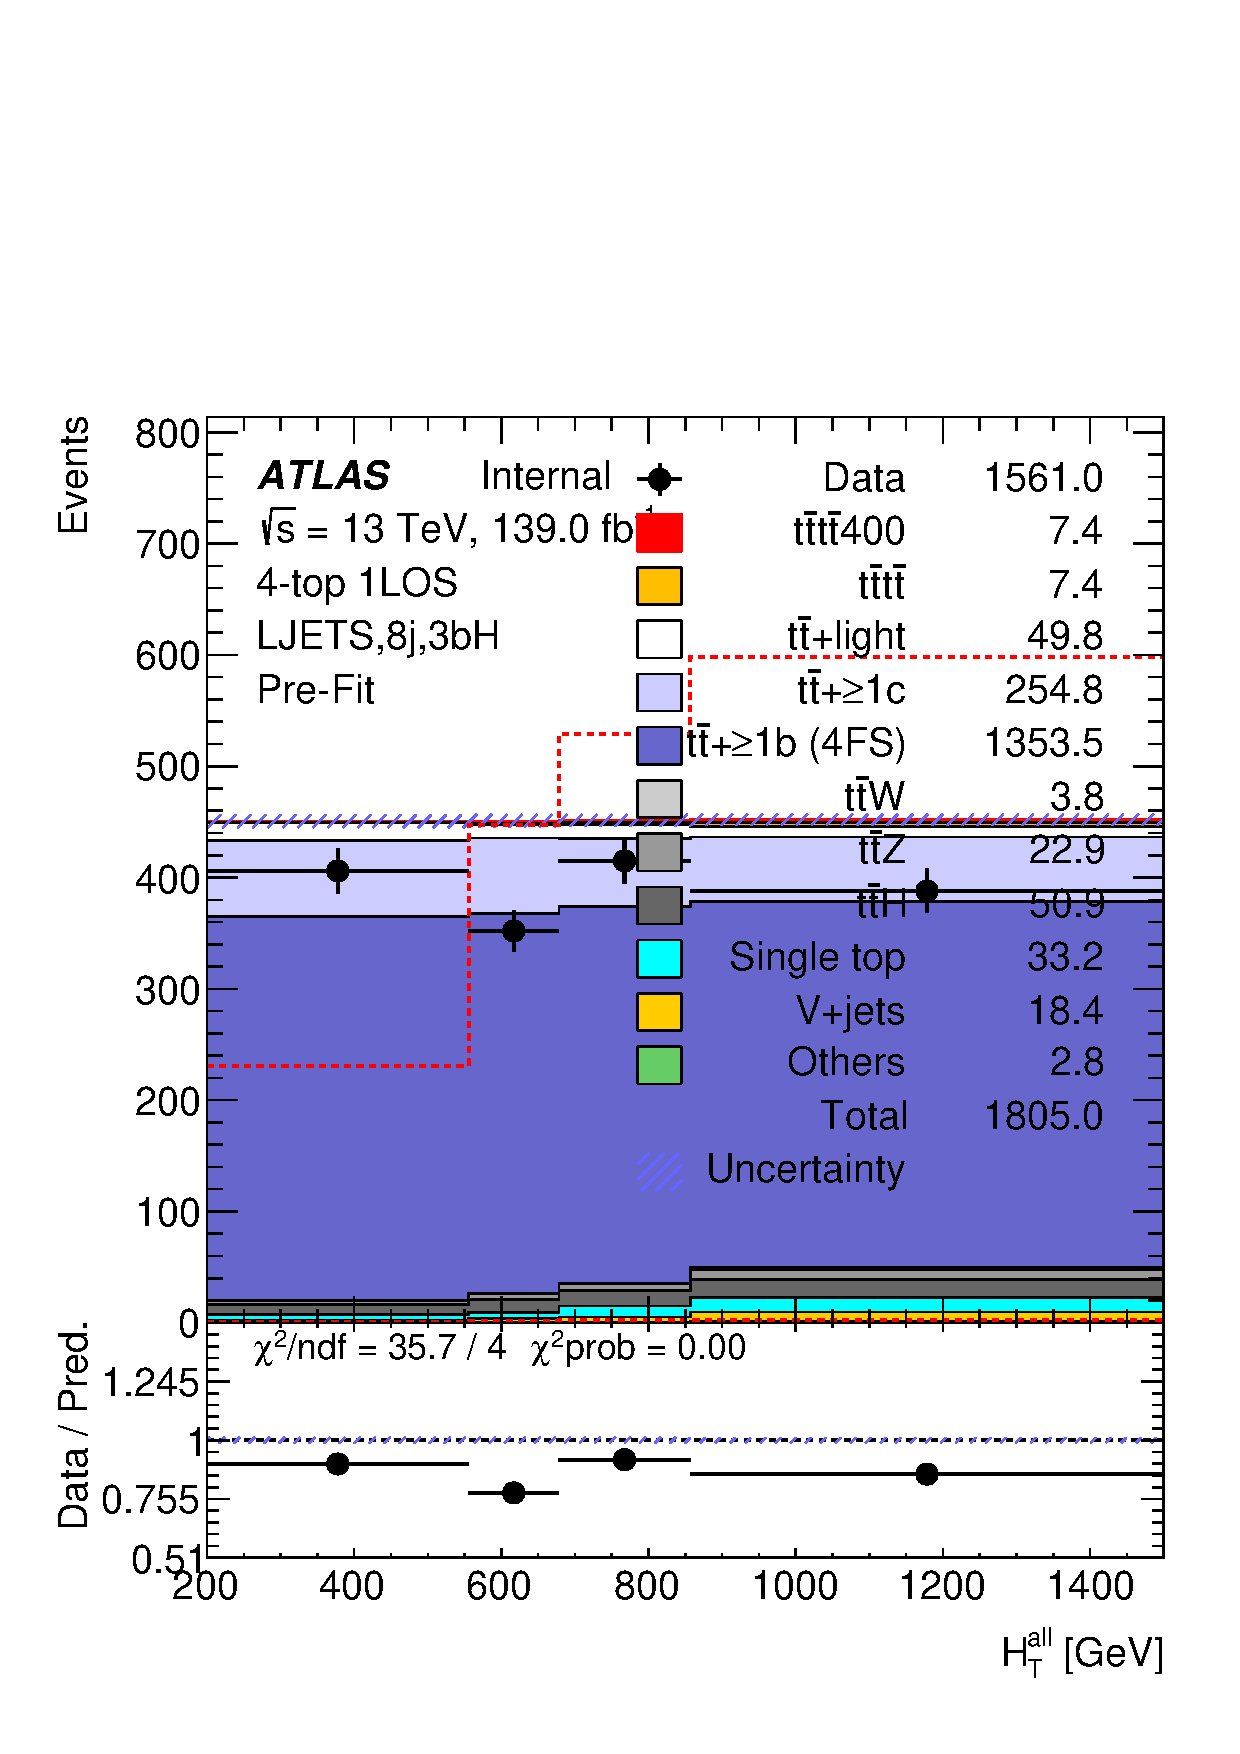
\includegraphics[width=0.25 \textwidth]{figures/fits/4FSvs5FS/GNN/400/Data_to_MC_4FS/ljets_8j3bH.pdf} &
        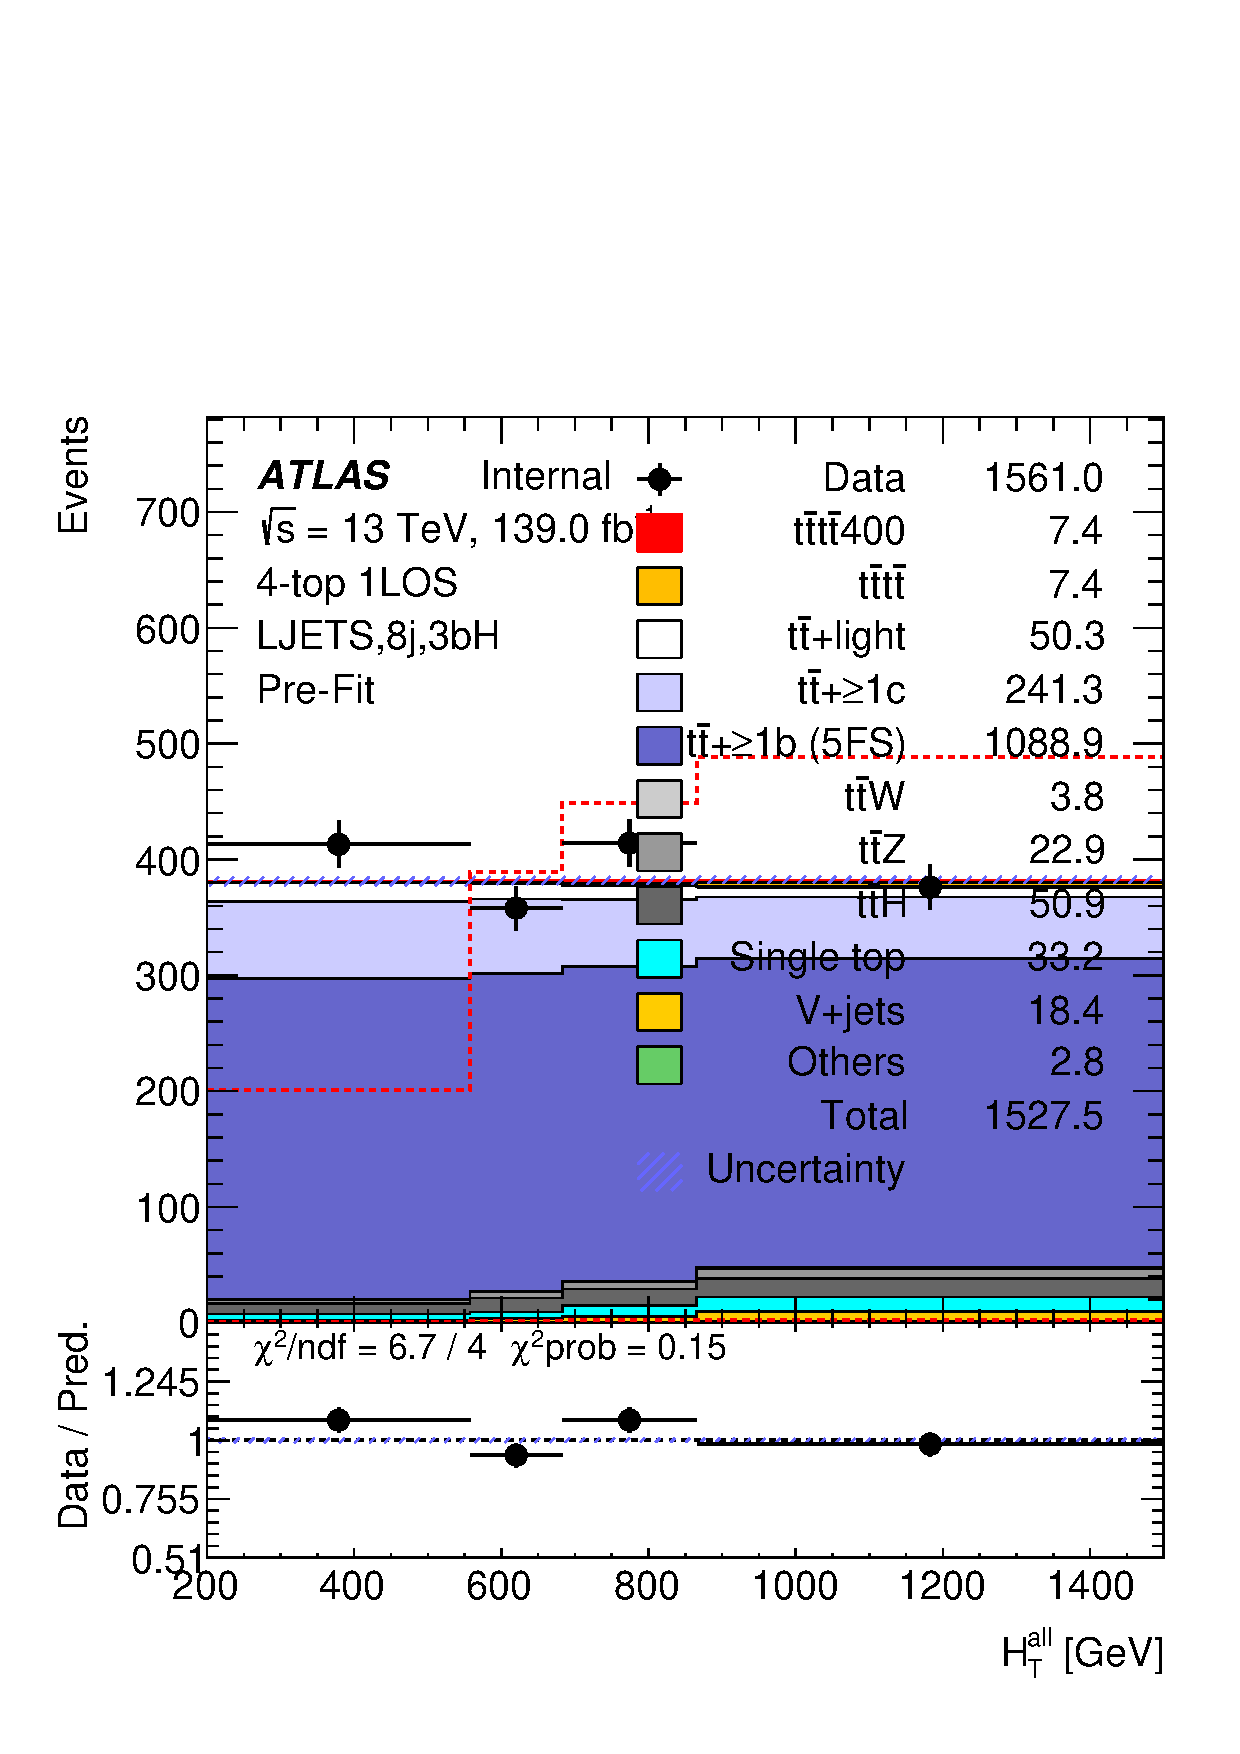
\includegraphics[width=0.25 \textwidth]{figures/fits/4FSvs5FS/GNN/400/Data_to_MC_5FS/ljets_8j3bH.pdf} &
        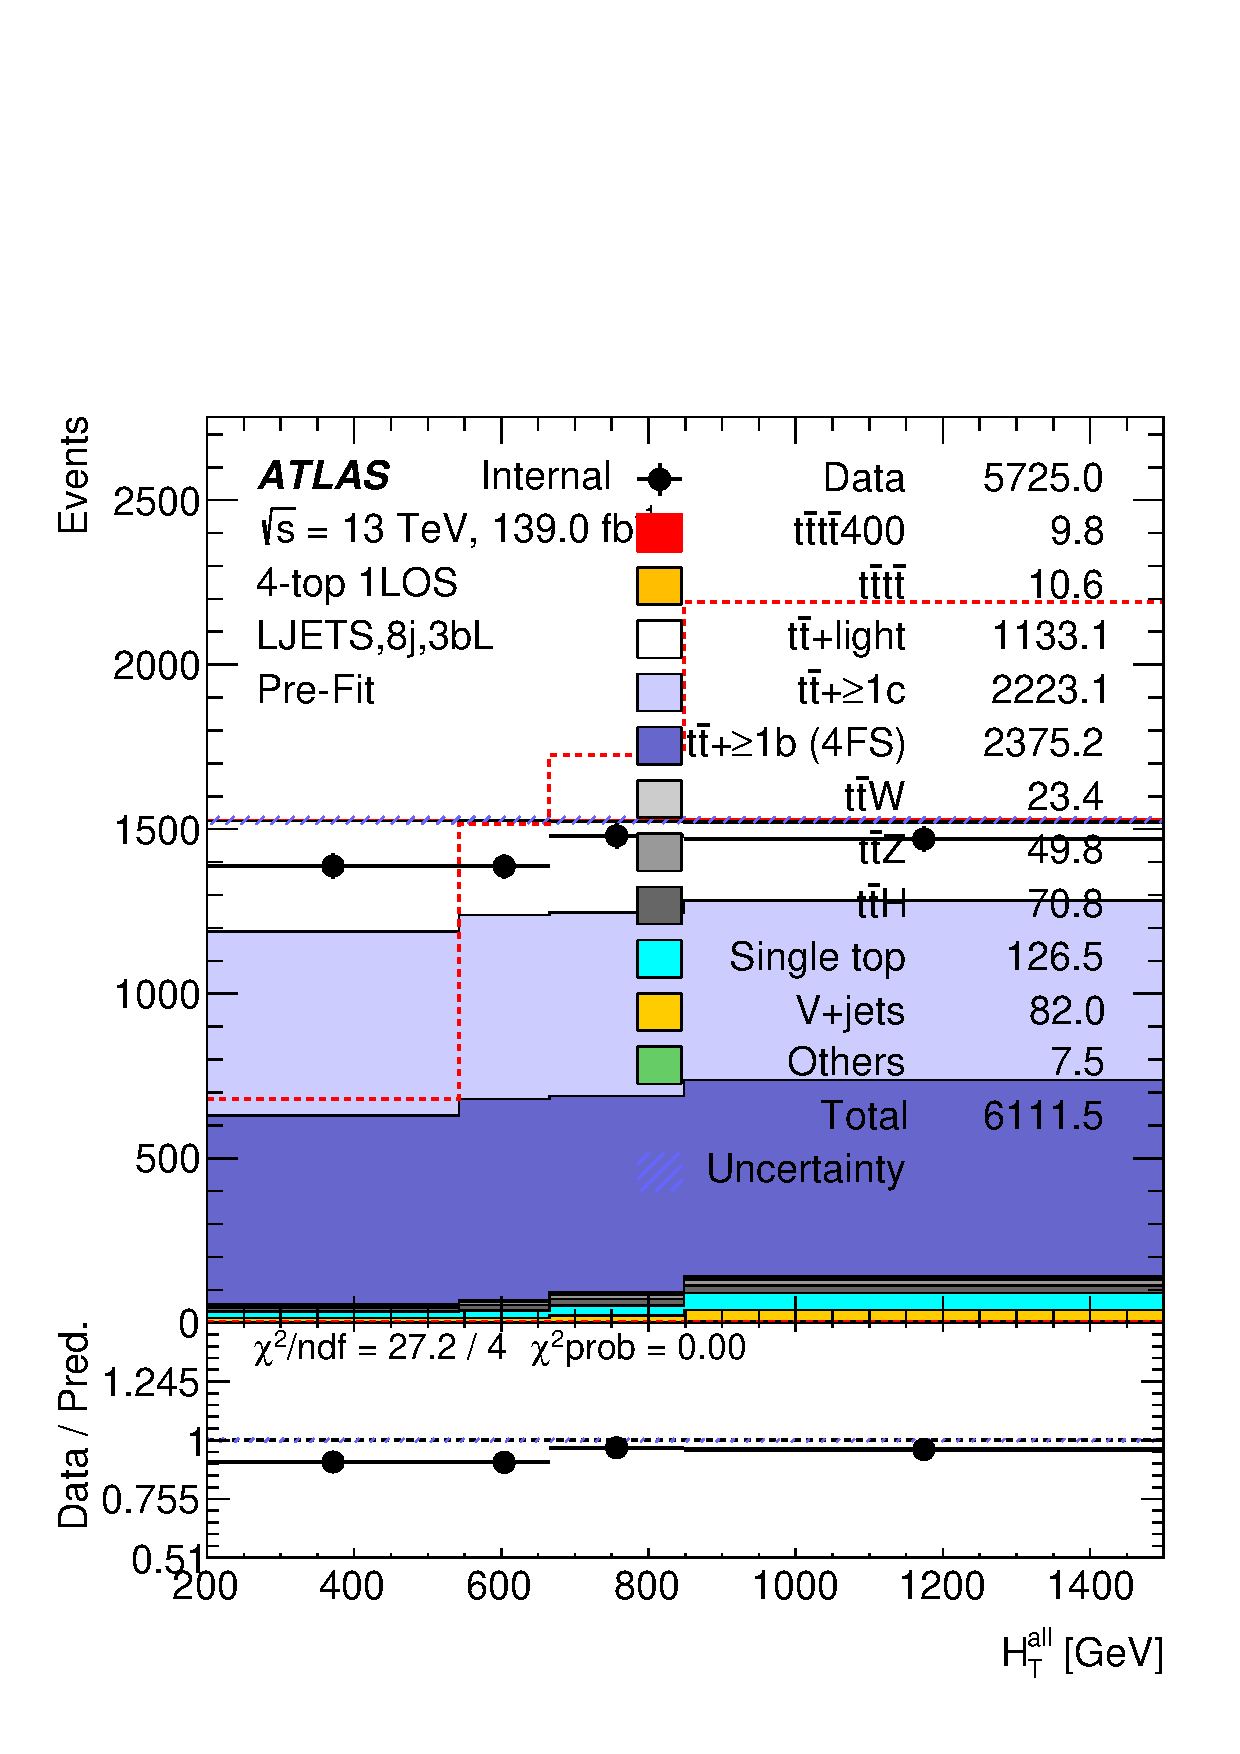
\includegraphics[width=0.25 \textwidth]{figures/fits/4FSvs5FS/GNN/400/Data_to_MC_4FS/ljets_8j3bL.pdf} &
        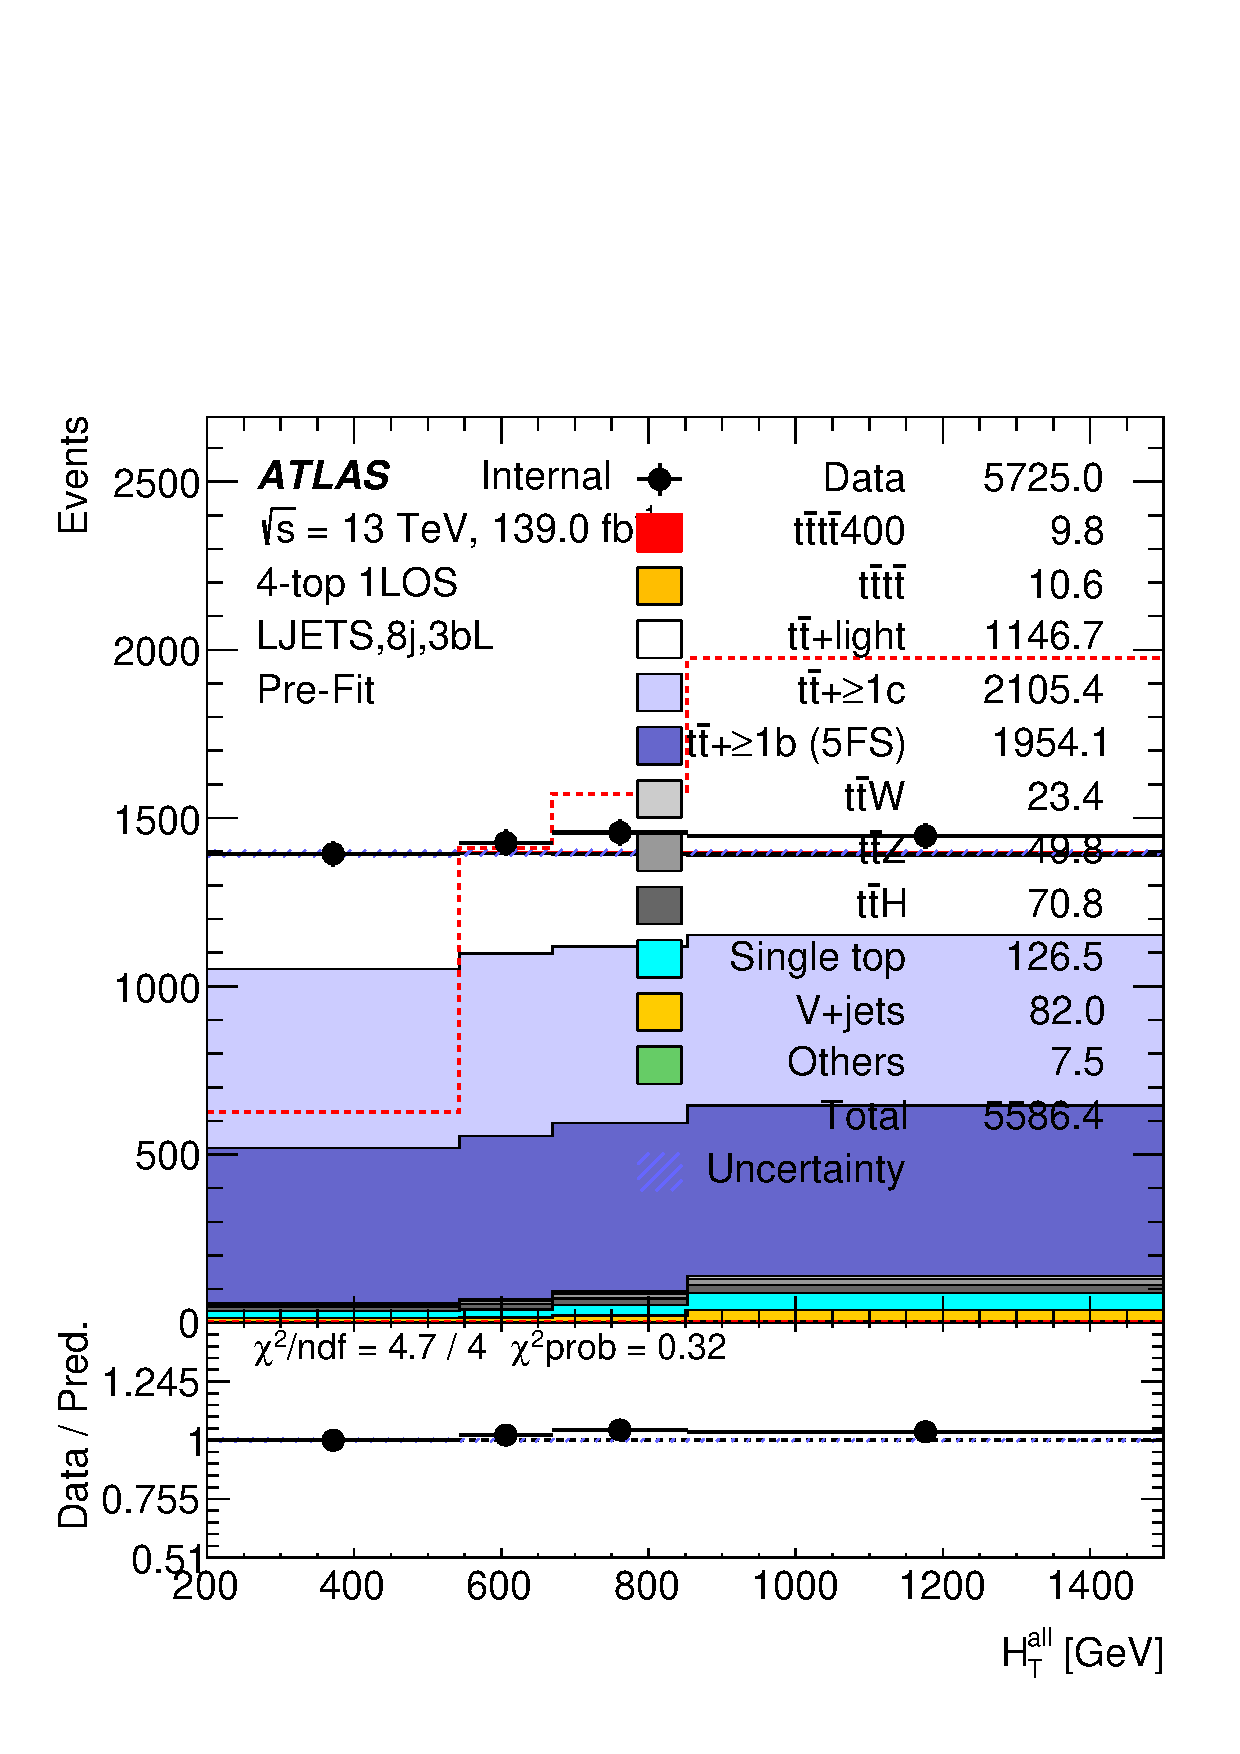
\includegraphics[width=0.25 \textwidth]{figures/fits/4FSvs5FS/GNN/400/Data_to_MC_5FS/ljets_8j3bL.pdf}\\

        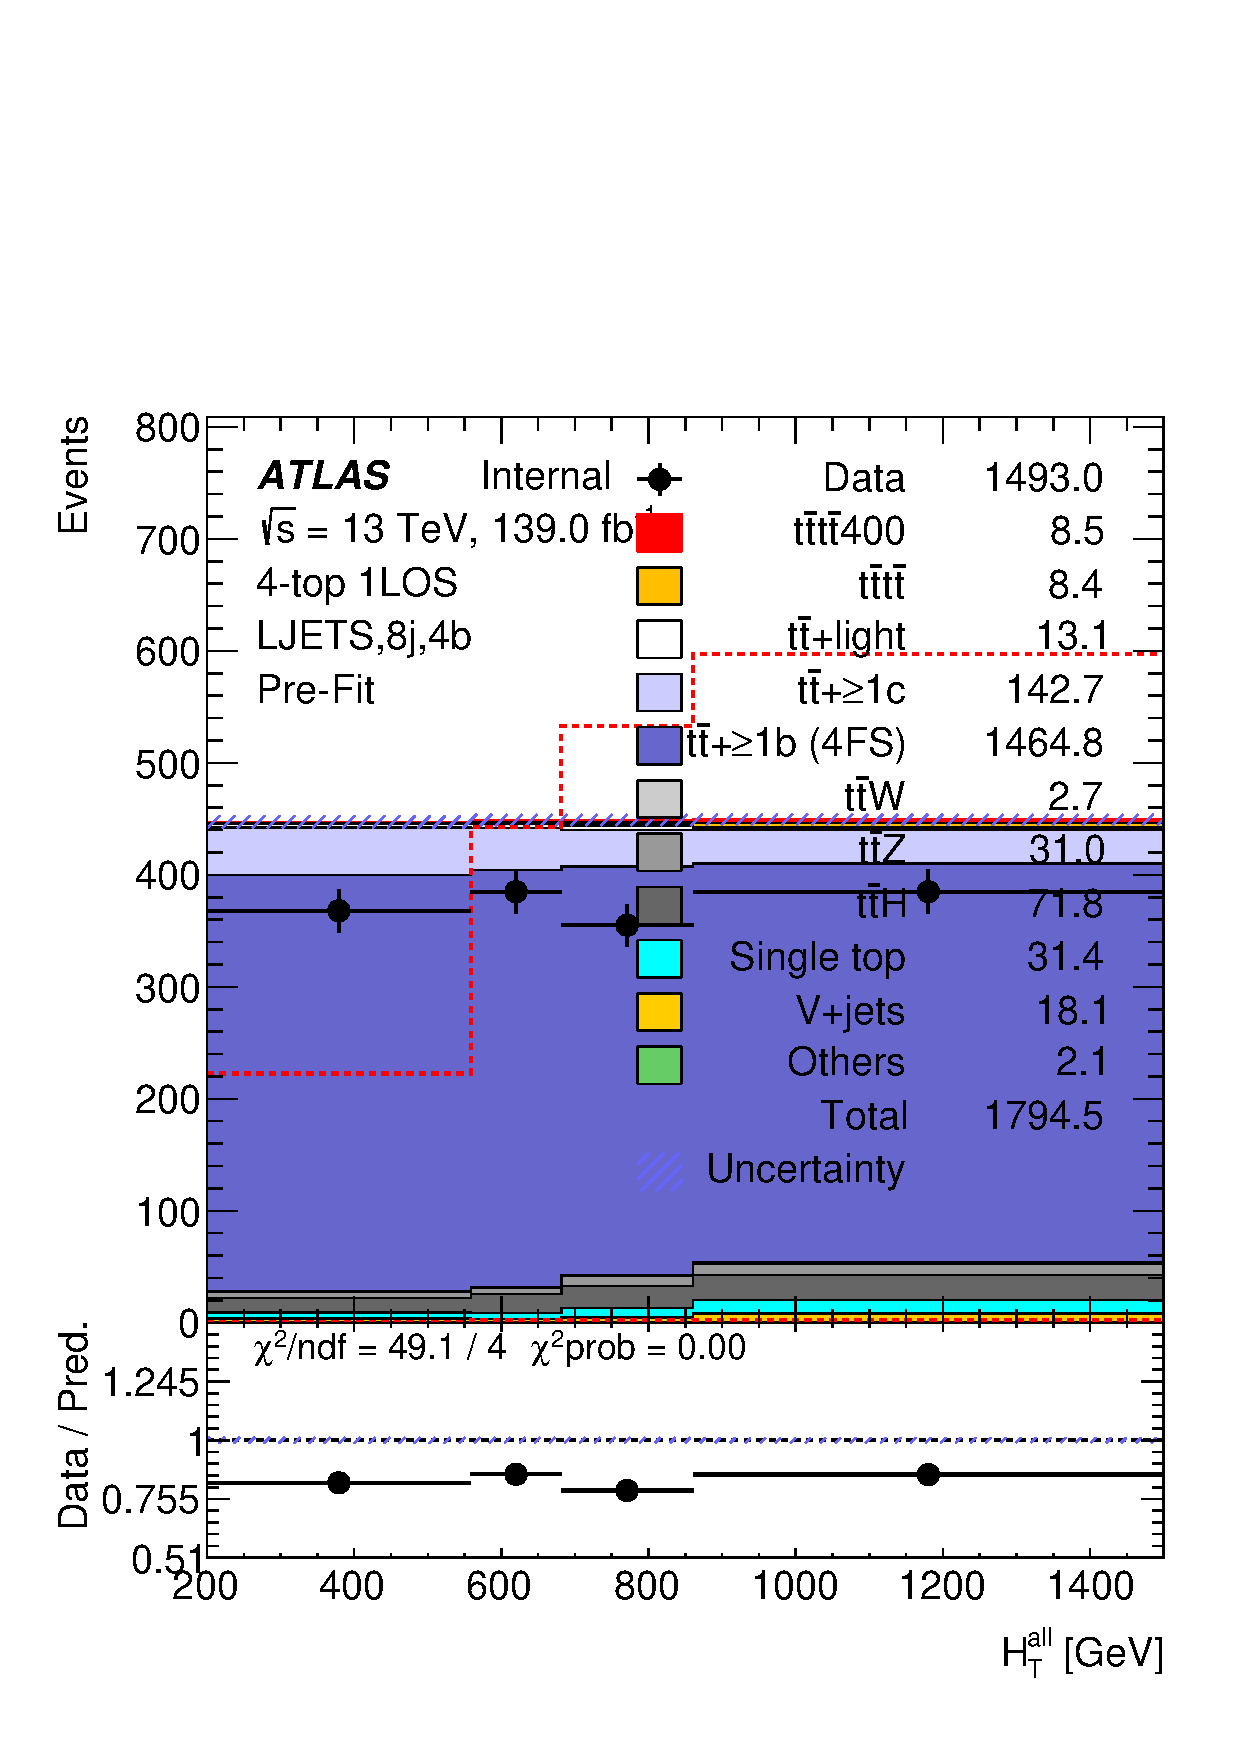
\includegraphics[width=0.25 \textwidth]{figures/fits/4FSvs5FS/GNN/400/Data_to_MC_4FS/ljets_8j4b.pdf} &
        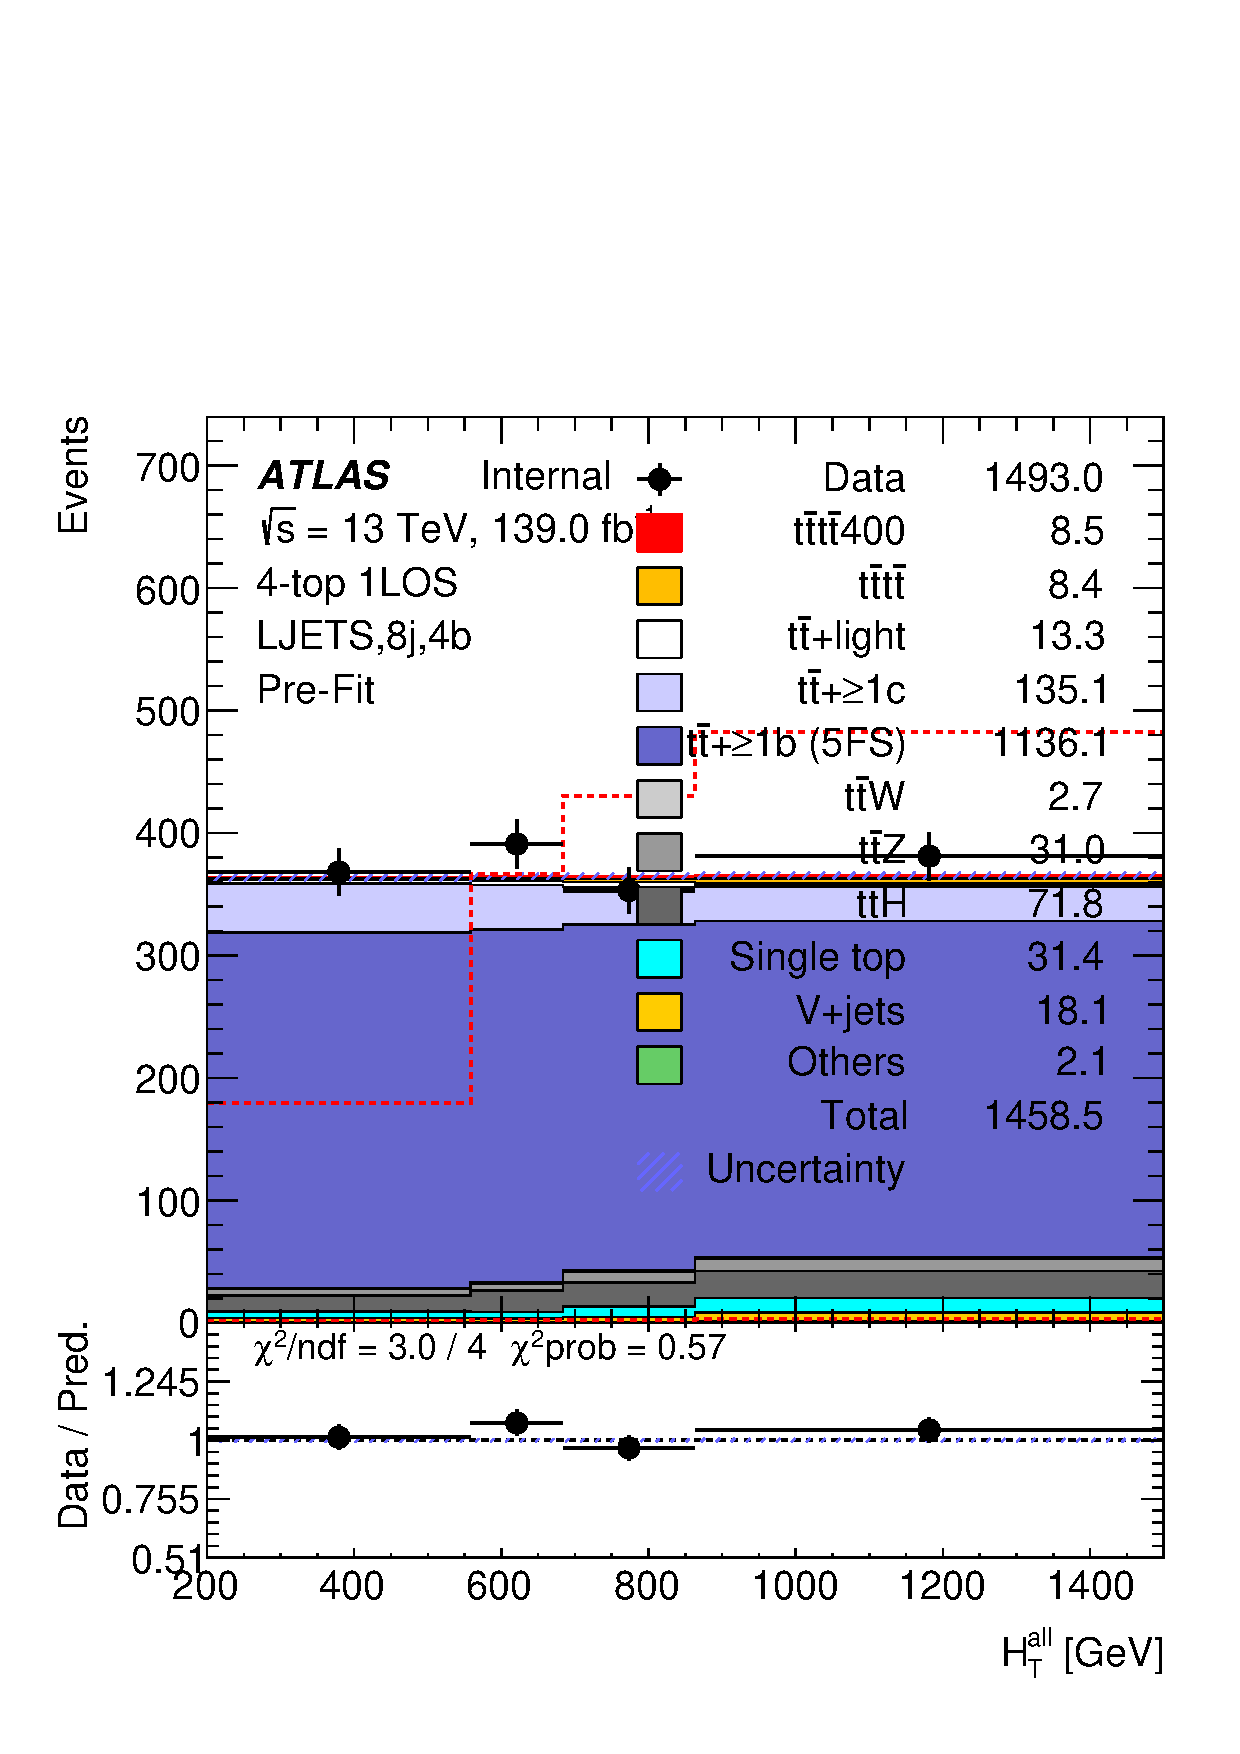
\includegraphics[width=0.25 \textwidth]{figures/fits/4FSvs5FS/GNN/400/Data_to_MC_5FS/ljets_8j4b.pdf} &
        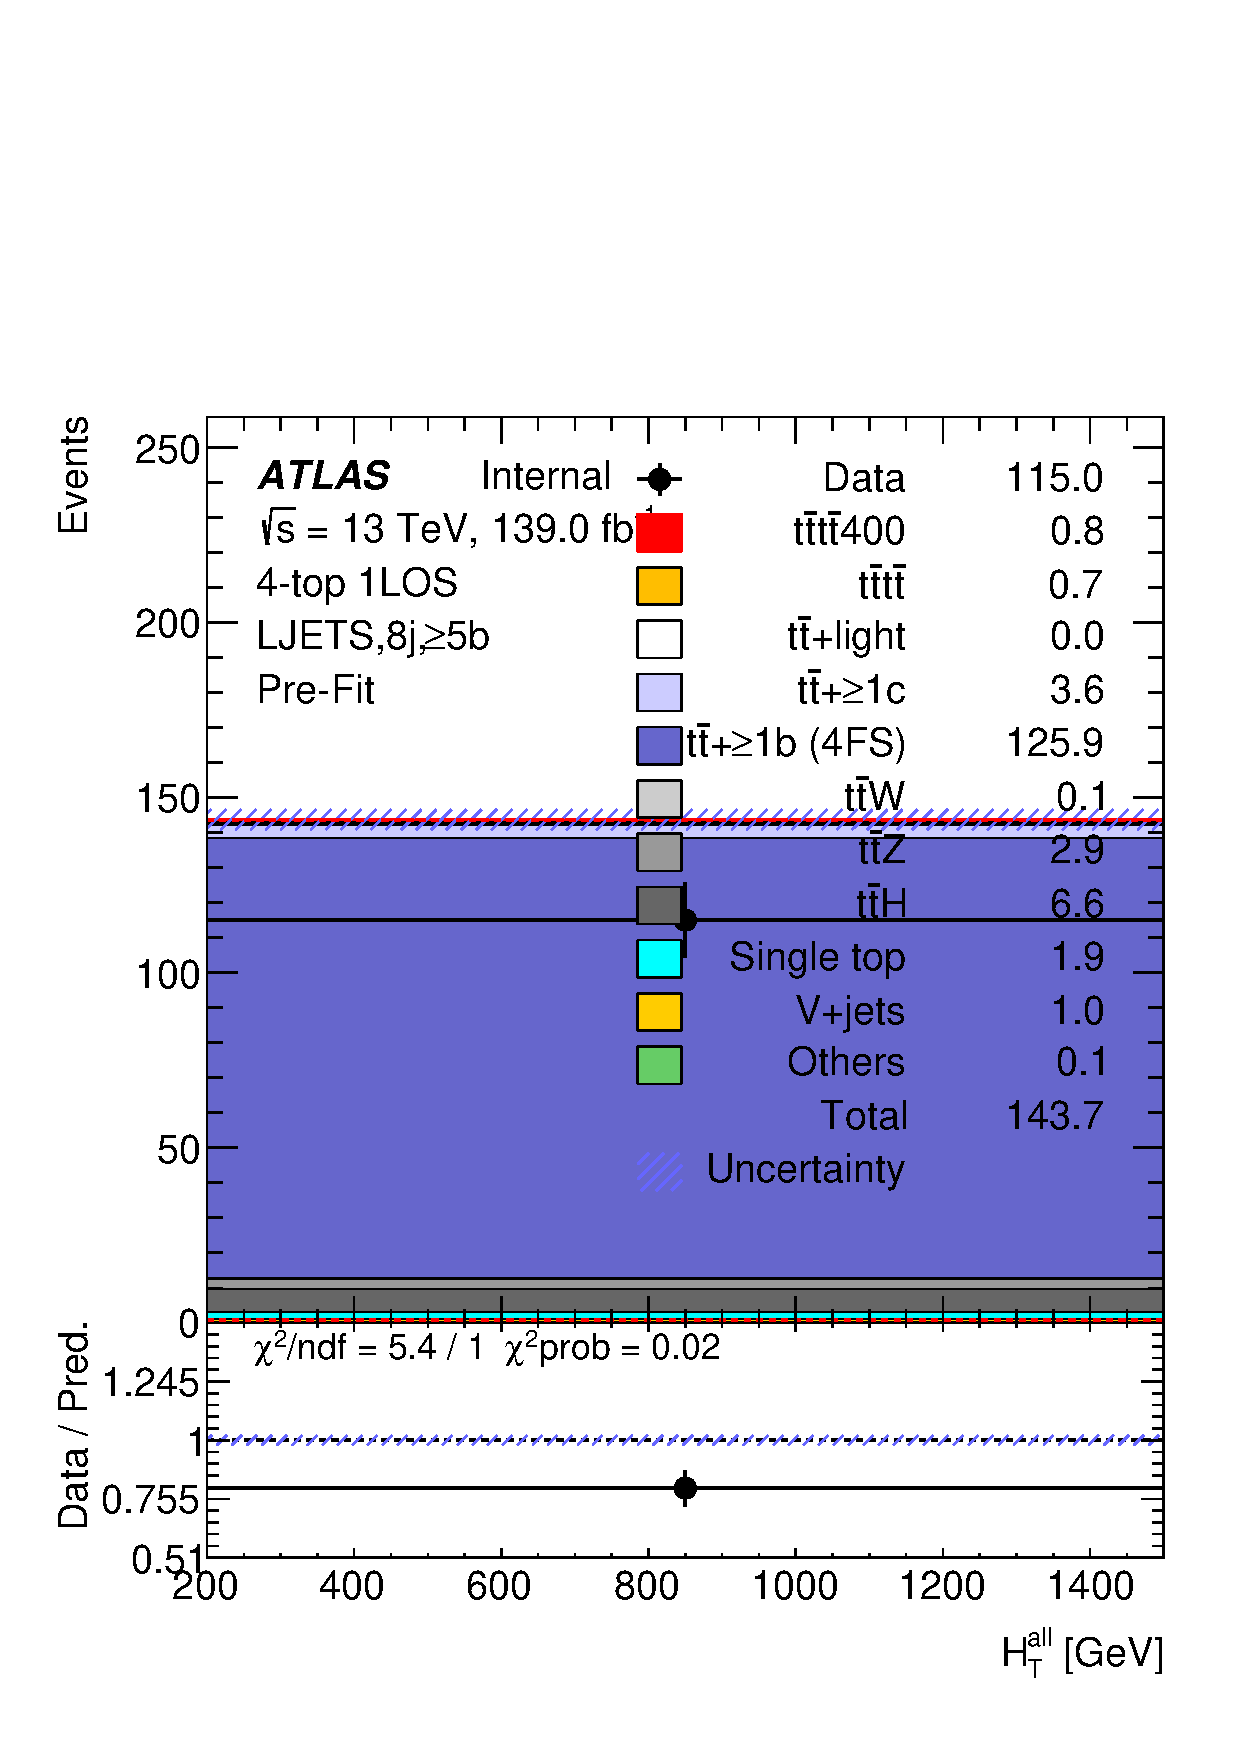
\includegraphics[width=0.25 \textwidth]{figures/fits/4FSvs5FS/GNN/400/Data_to_MC_4FS/ljets_8jge5b.pdf} &
        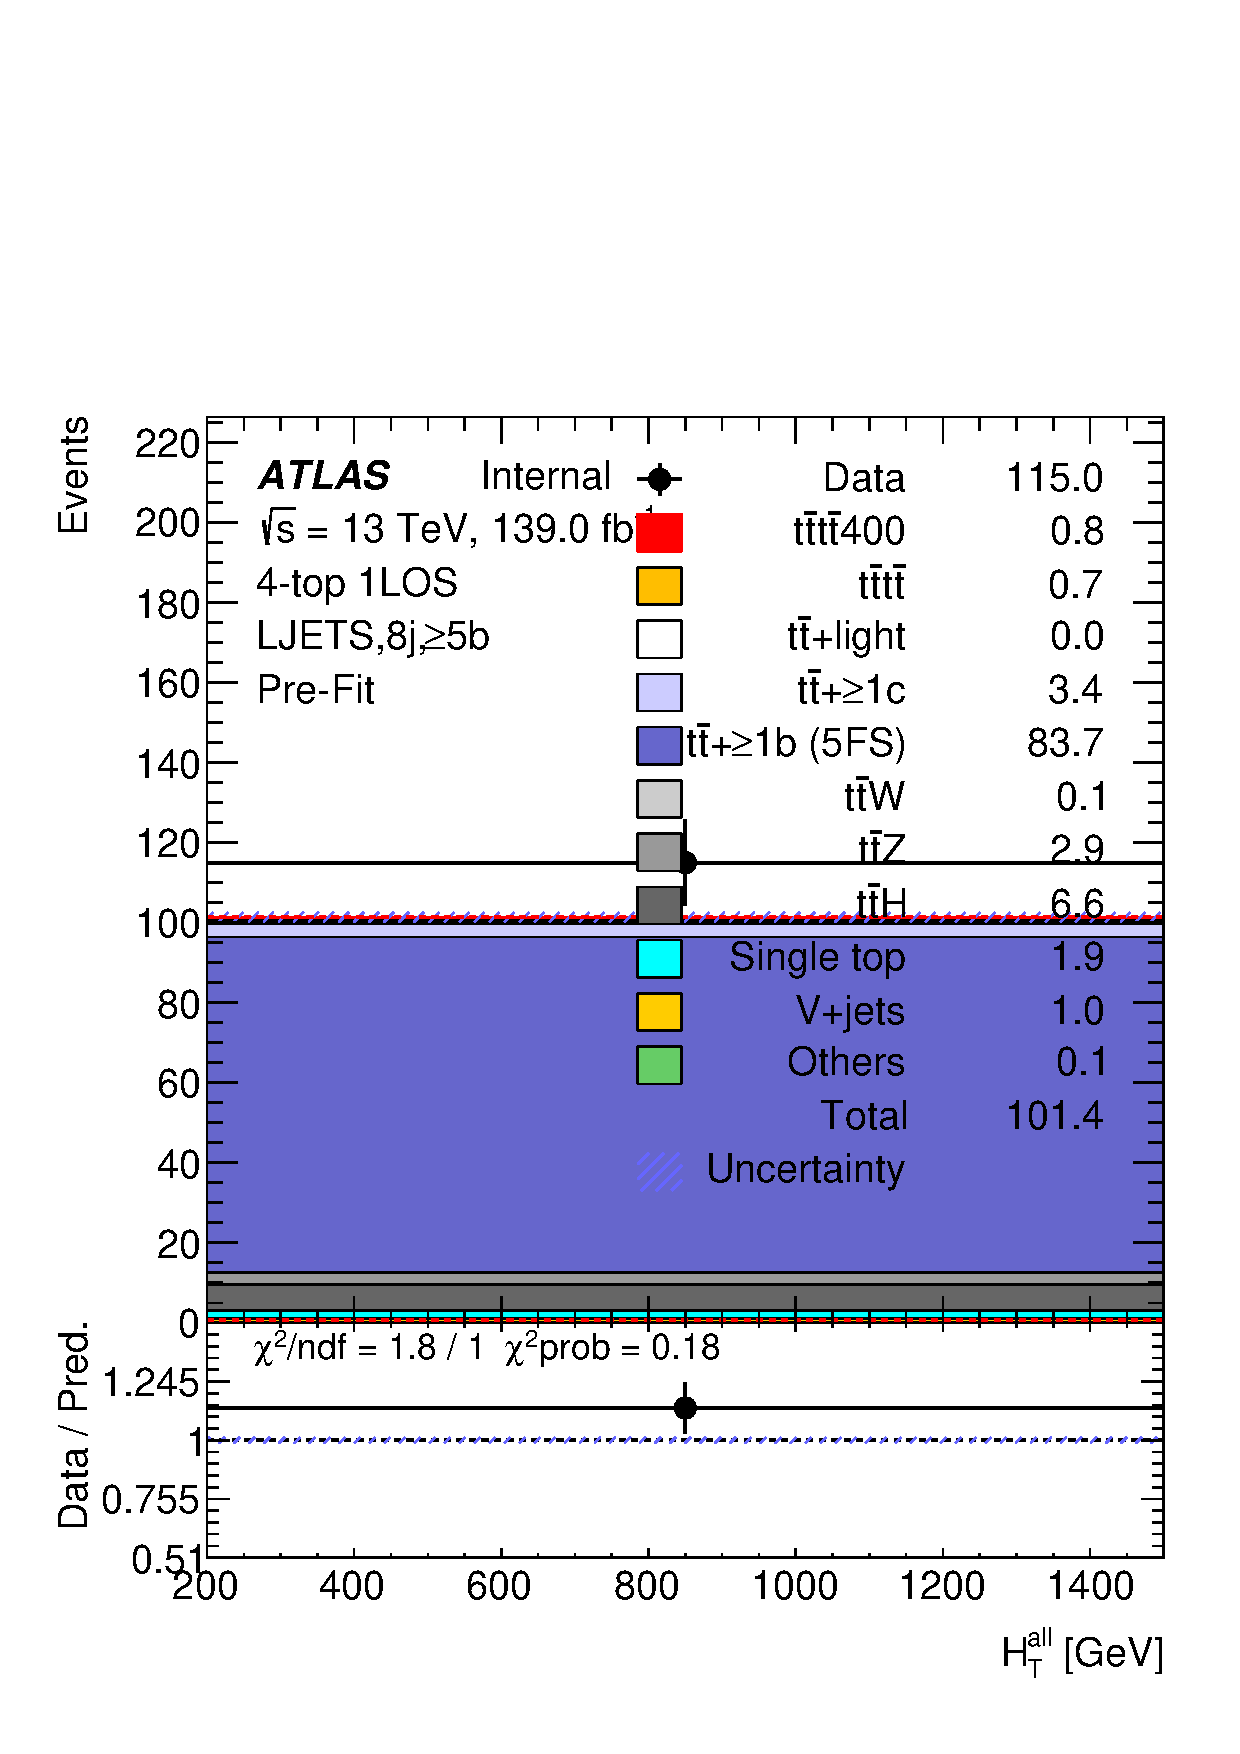
\includegraphics[width=0.25 \textwidth]{figures/fits/4FSvs5FS/GNN/400/Data_to_MC_5FS/ljets_8jge5b.pdf} \\

        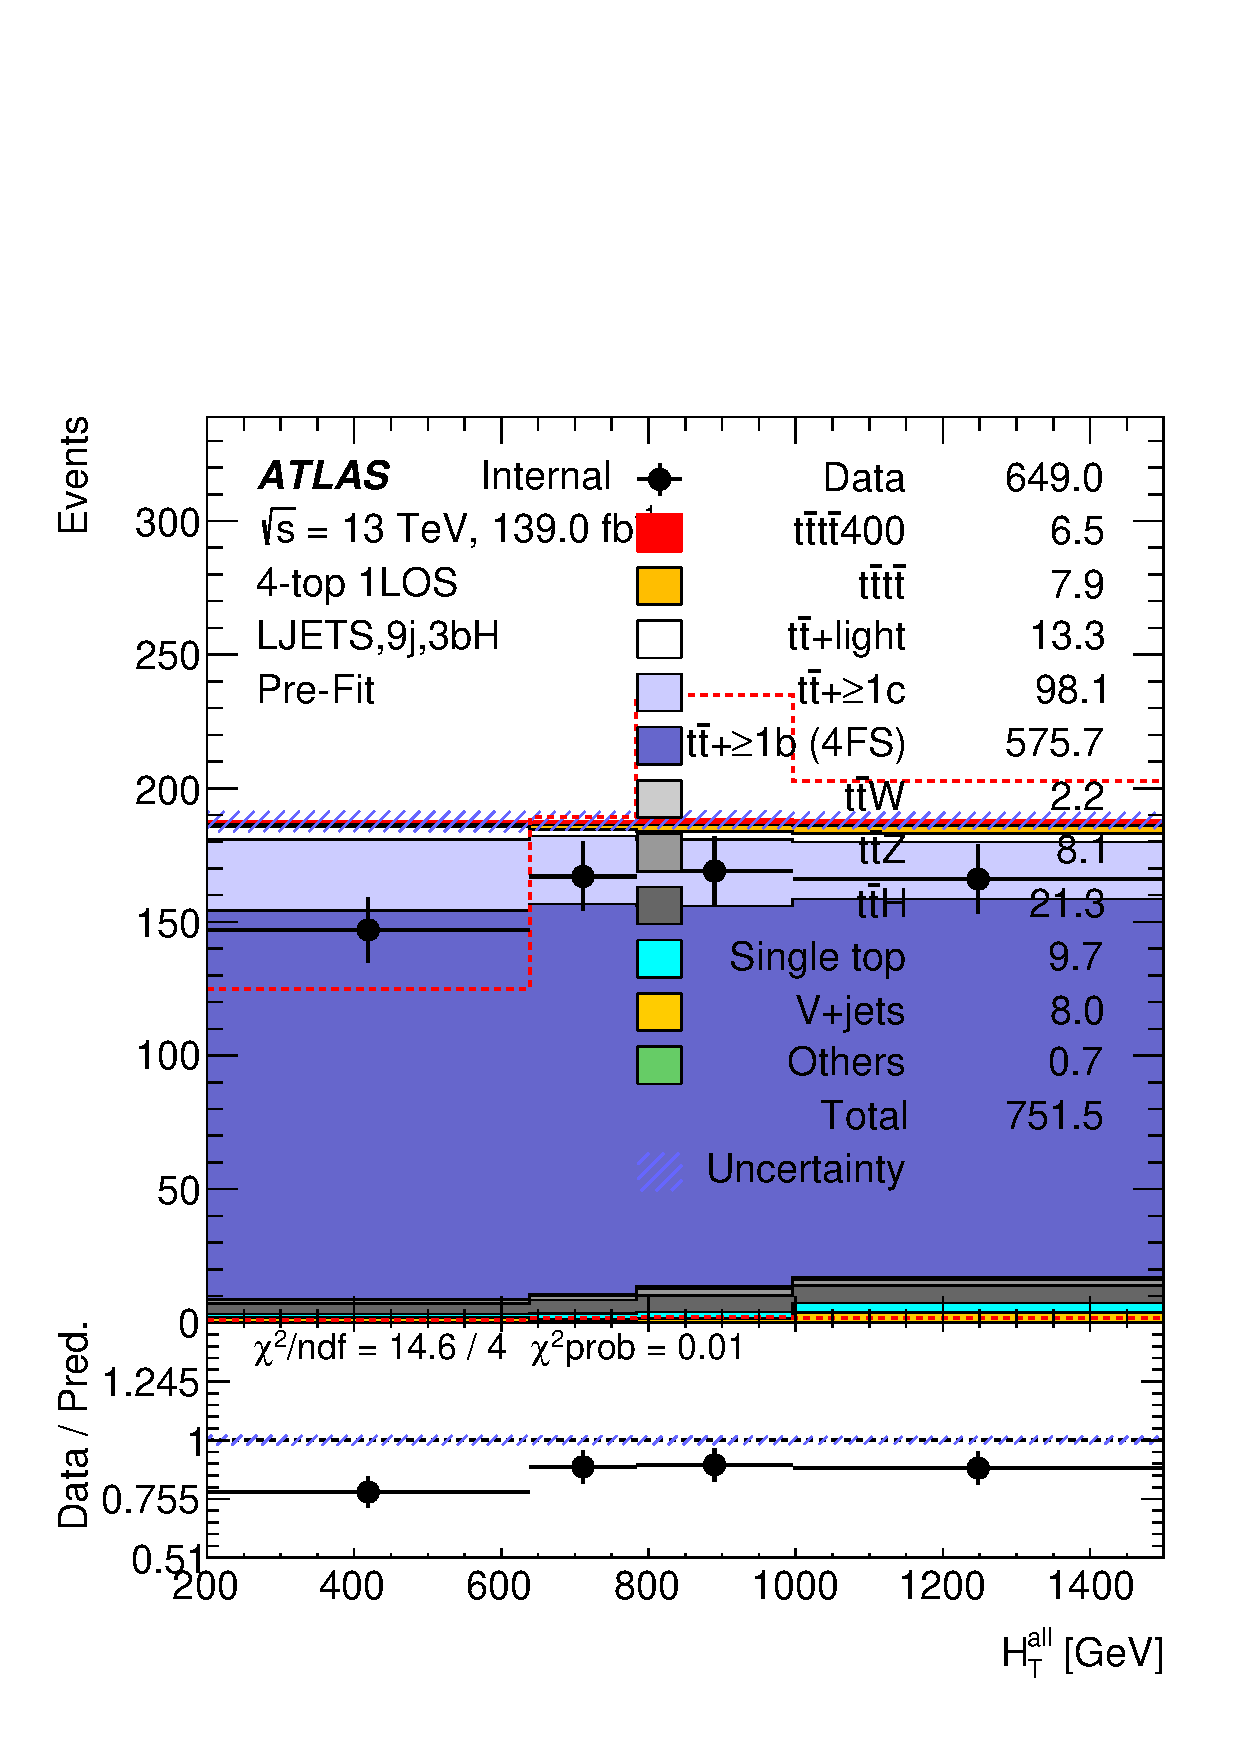
\includegraphics[width=0.25 \textwidth]{figures/fits/4FSvs5FS/GNN/400/Data_to_MC_4FS/ljets_9j3bH.pdf} &
        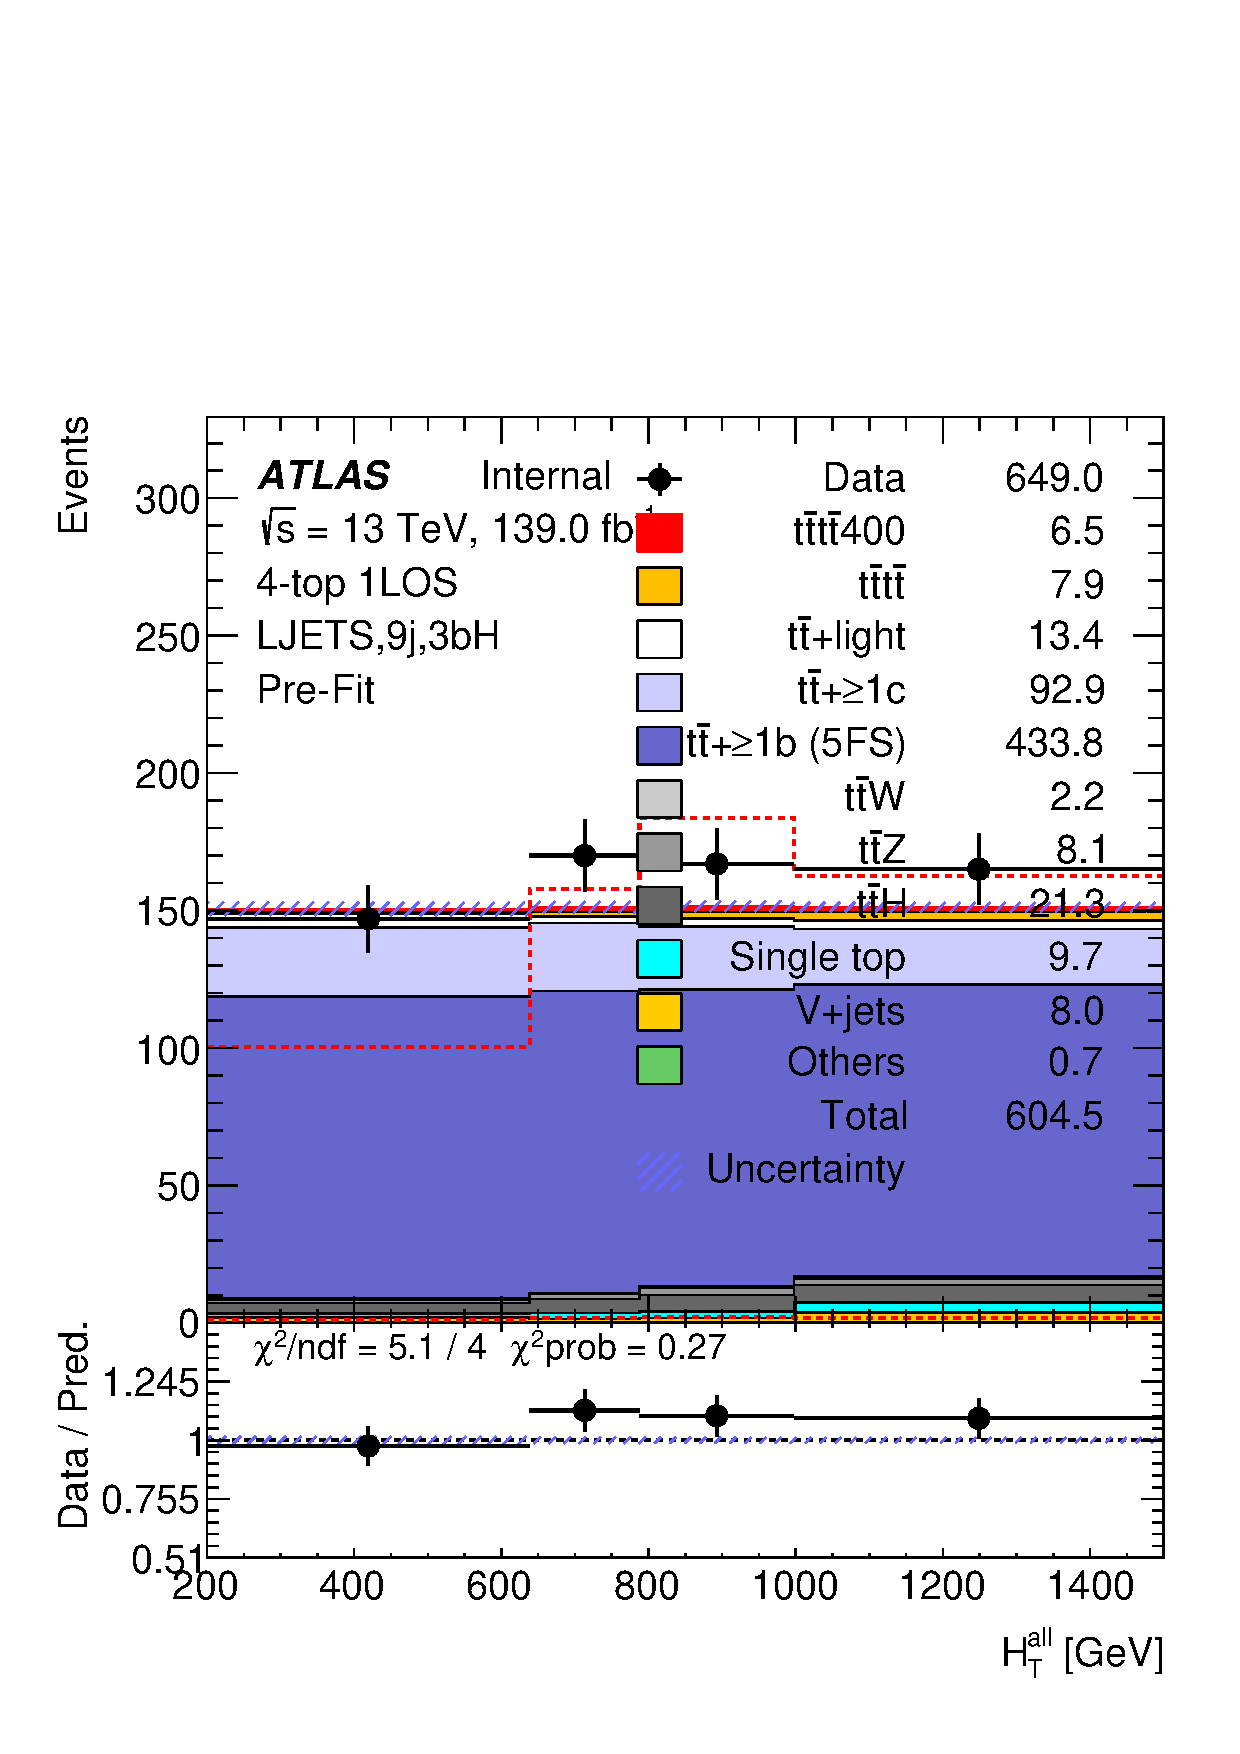
\includegraphics[width=0.25 \textwidth]{figures/fits/4FSvs5FS/GNN/400/Data_to_MC_5FS/ljets_9j3bH.pdf} &
        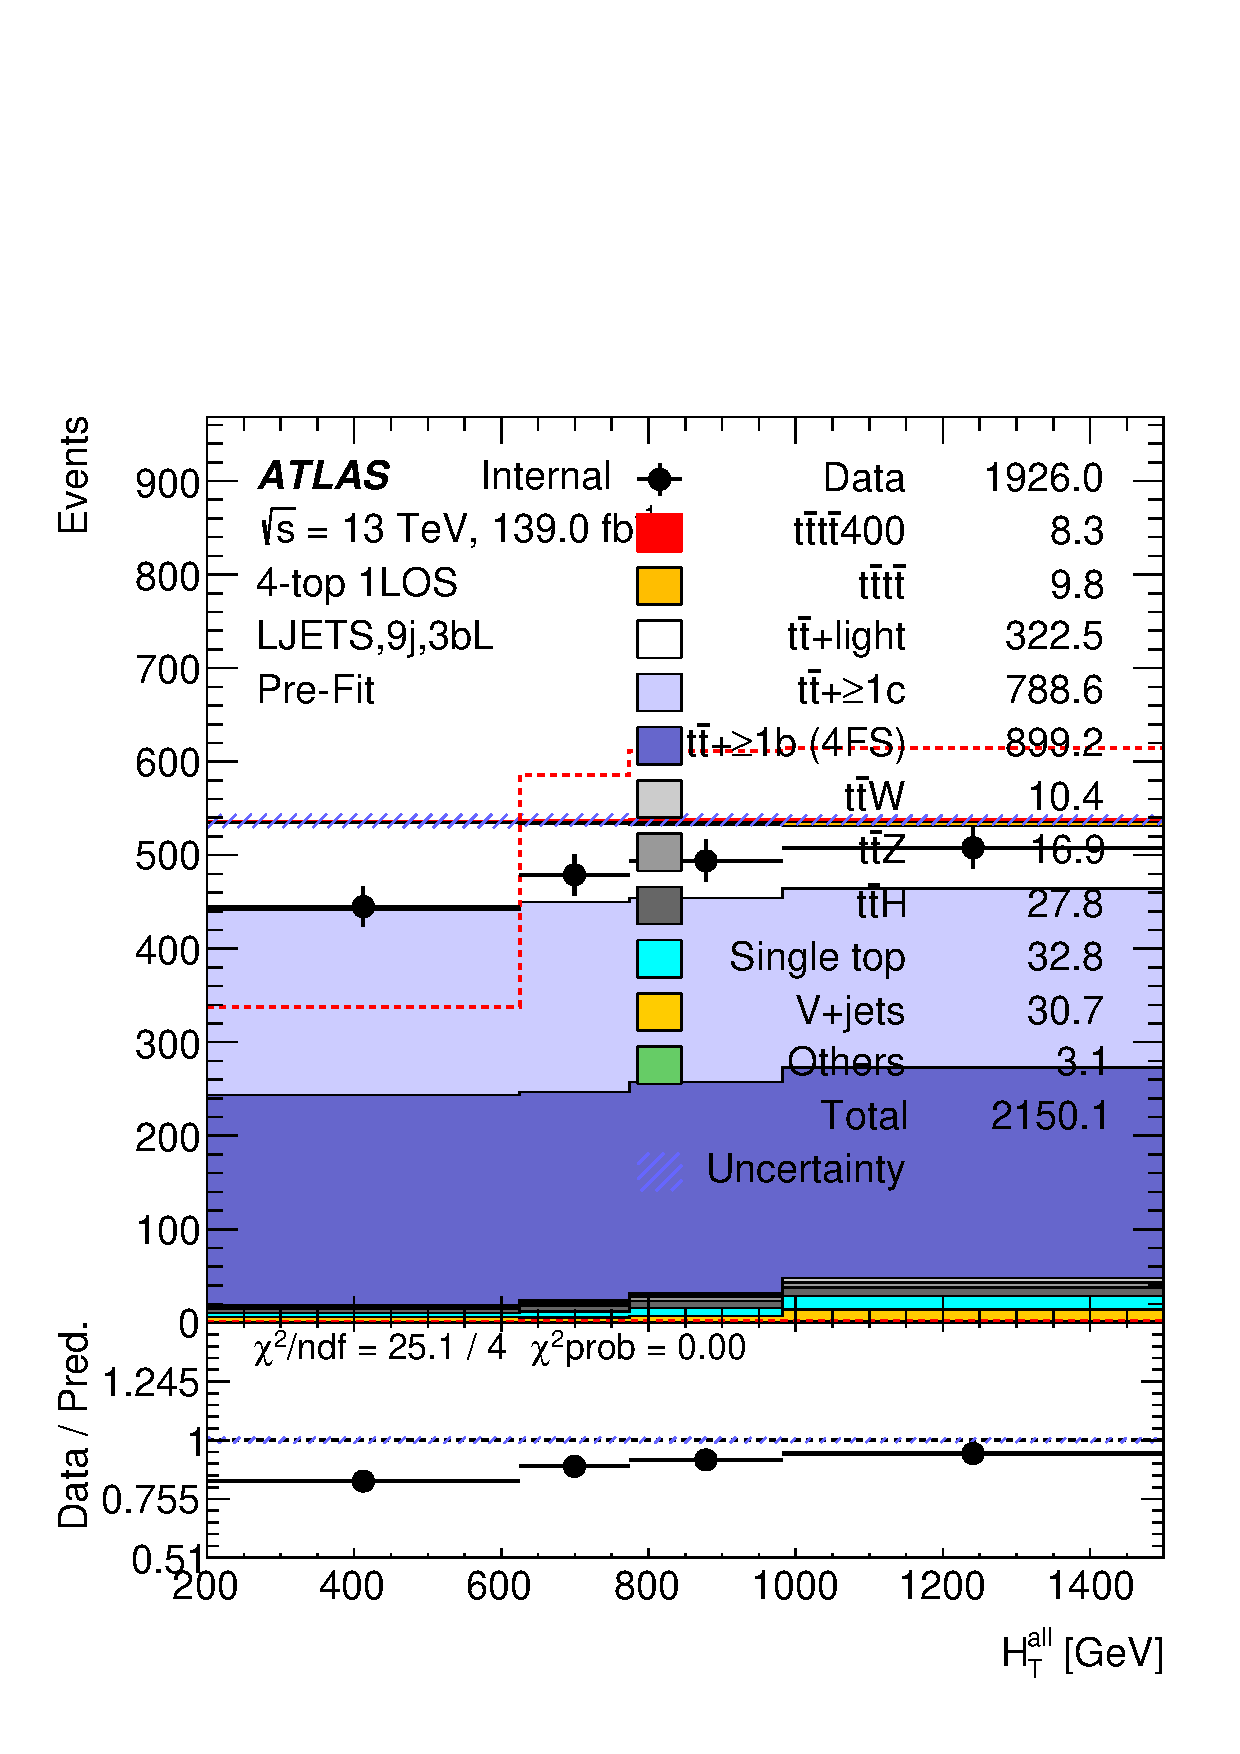
\includegraphics[width=0.25 \textwidth]{figures/fits/4FSvs5FS/GNN/400/Data_to_MC_4FS/ljets_9j3bL.pdf} &
        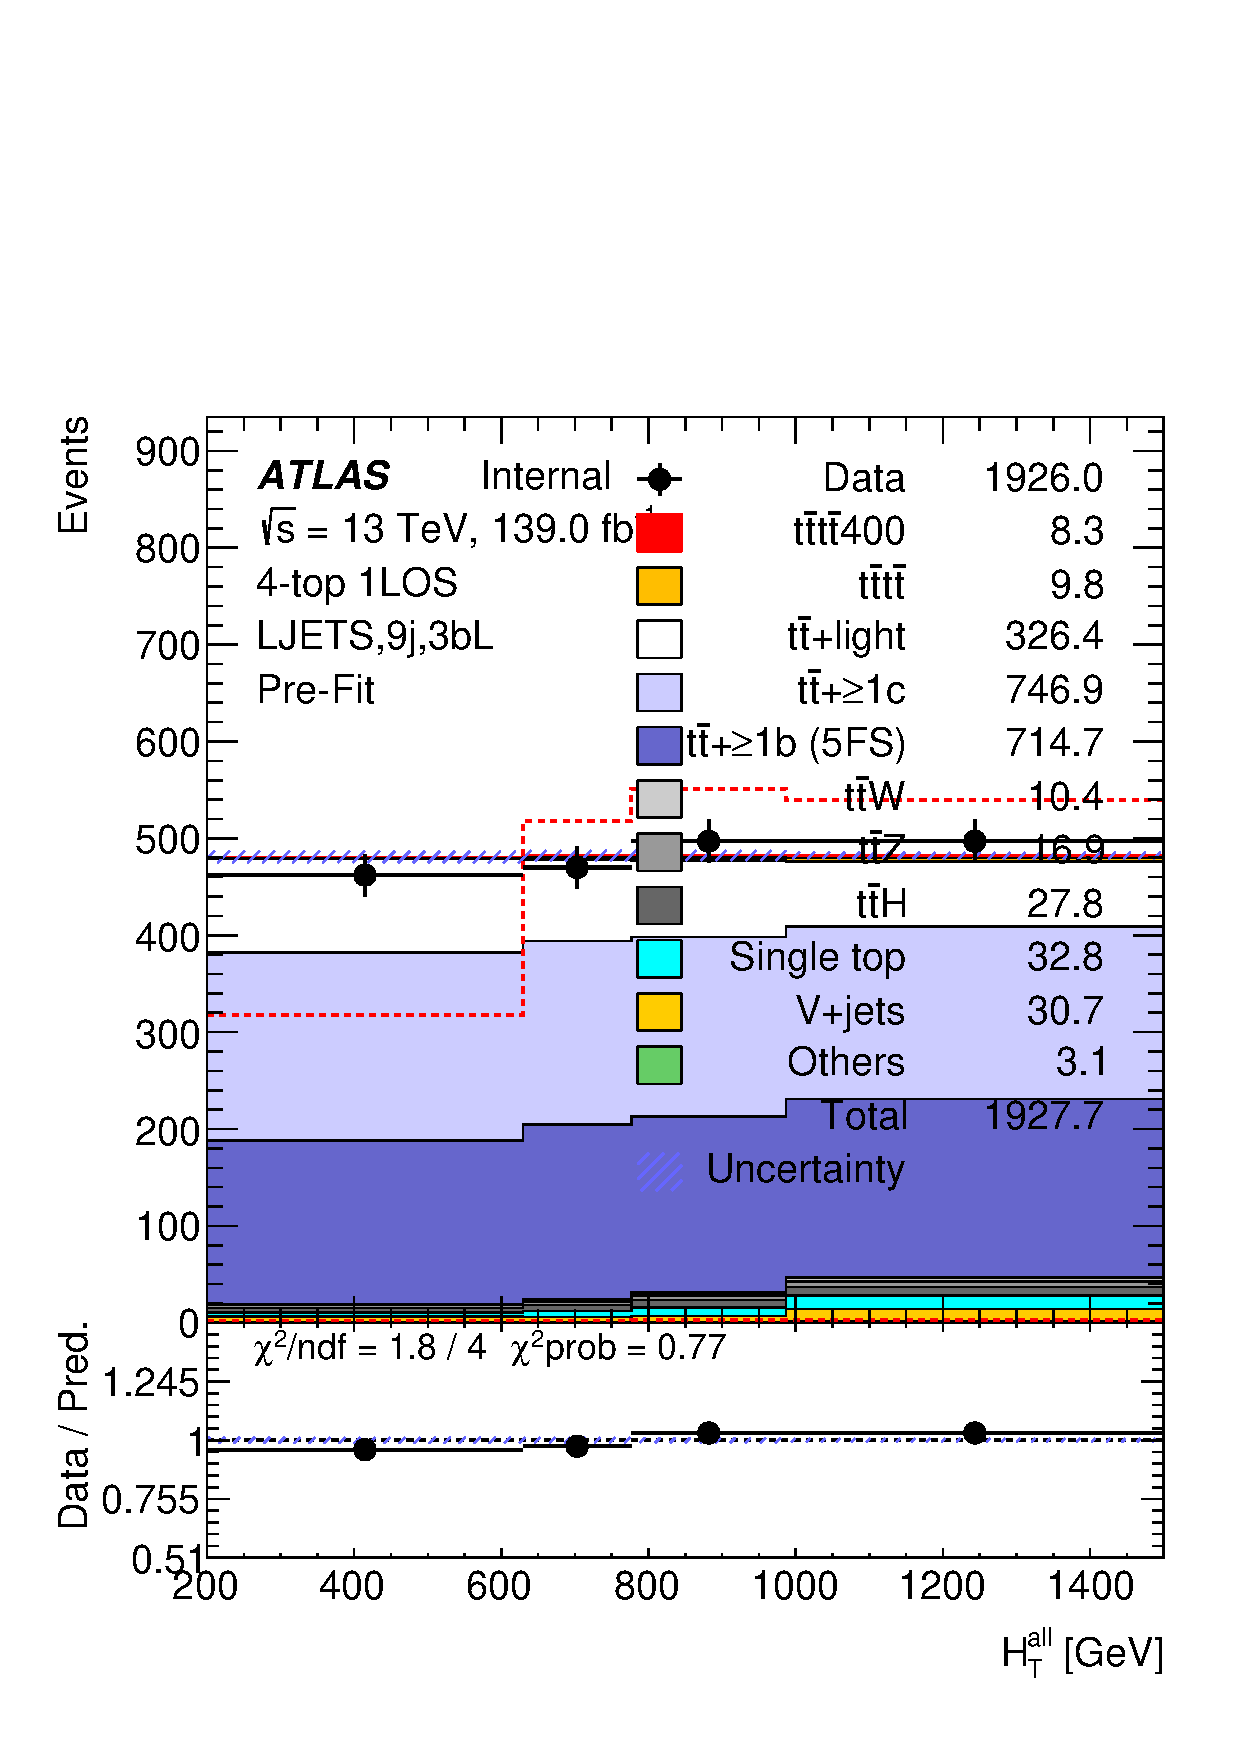
\includegraphics[width=0.25 \textwidth]{figures/fits/4FSvs5FS/GNN/400/Data_to_MC_5FS/ljets_9j3bL.pdf} \\
        \end{tabular}
        \caption{\label{4FSvs5FS_dataMC_1L}Pre-fit distributions in 5FS compared with 4FS for 1L channel associated with different signal and background samples, compared with data yields.}
\end{center}
\end{figure}

\begin{figure}[htbp!]                                                                                                                                                                   \begin{center} \setlength{\tabcolsep}{2.5pt}\footnotesize                                                                                                                 
        \begin{tabular}{cccc}                                                                            
        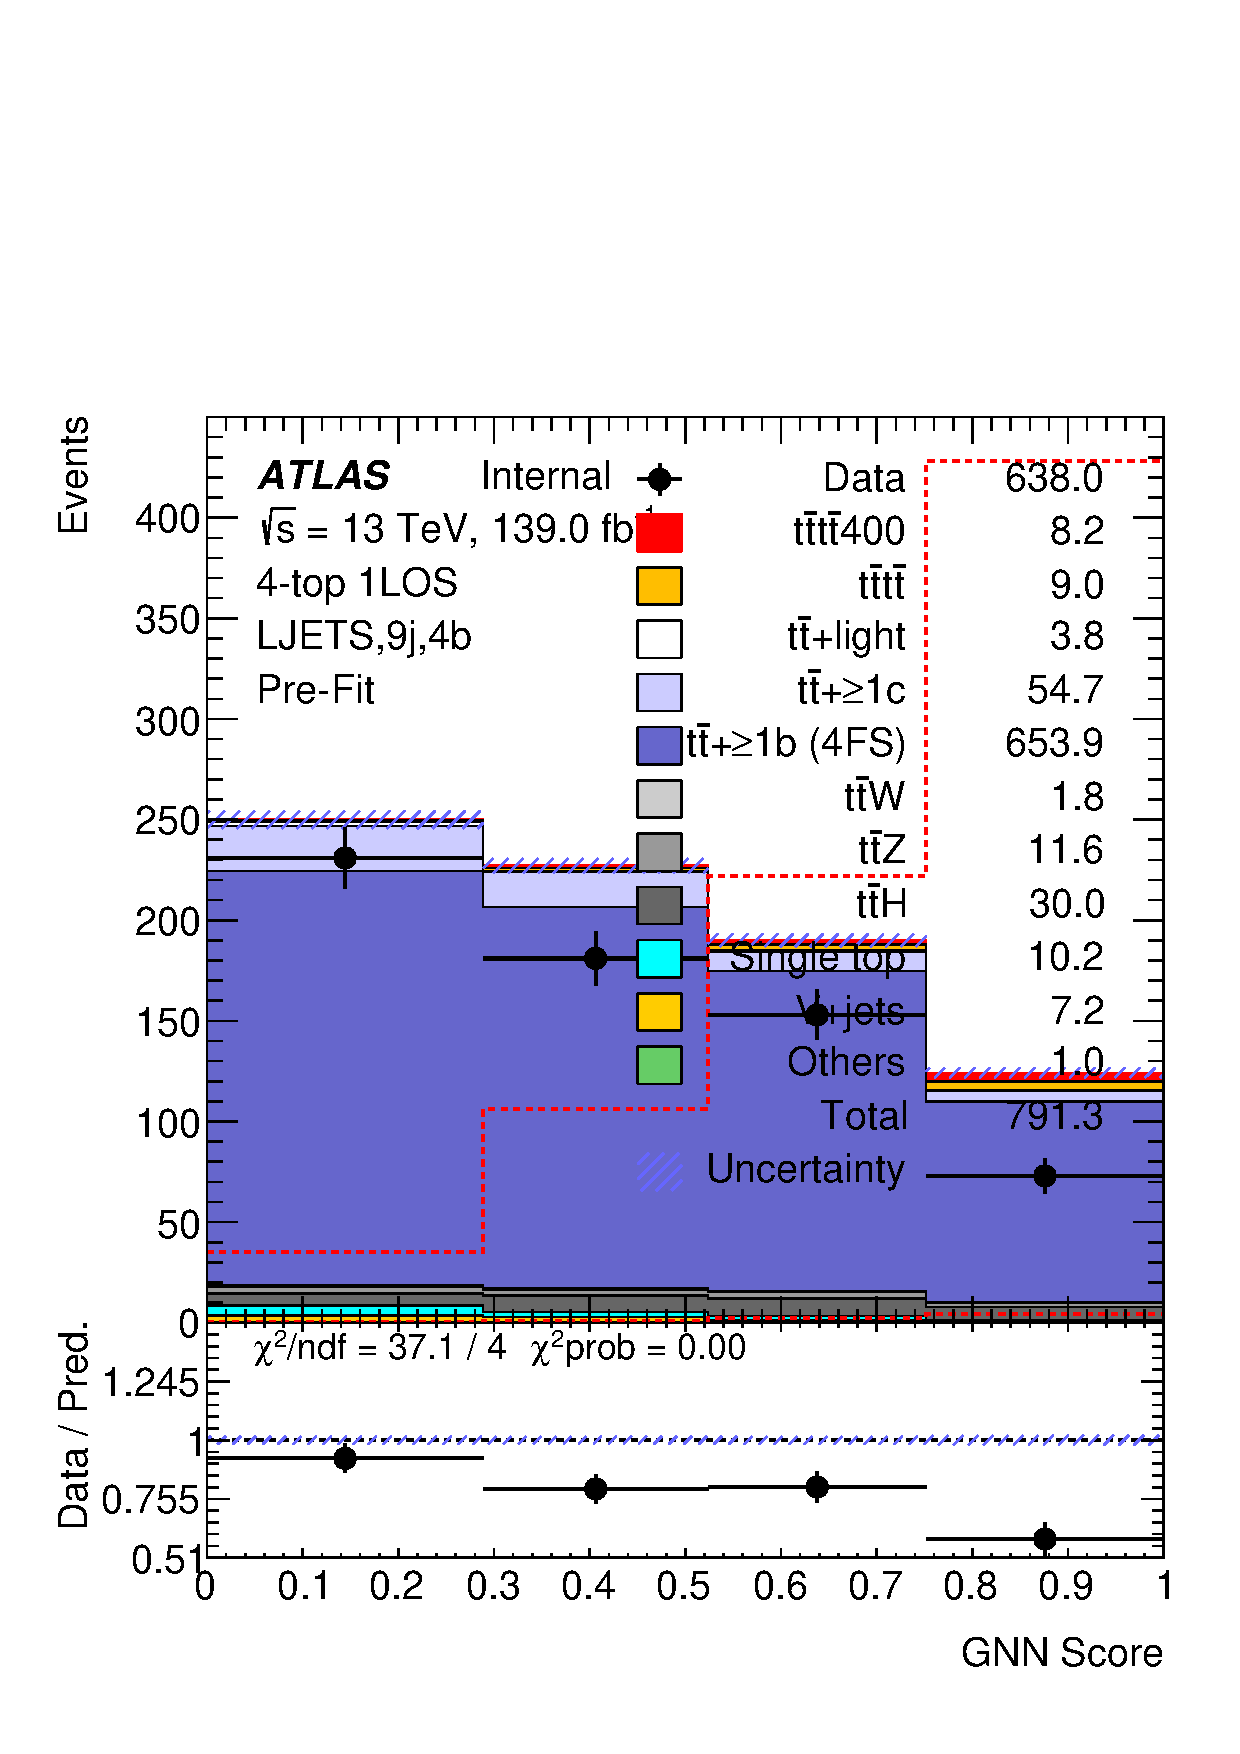
\includegraphics[width=0.25 \textwidth]{figures/fits/4FSvs5FS/GNN/400/Data_to_MC_4FS/ljets_9j4b.pdf} &                                                                     
        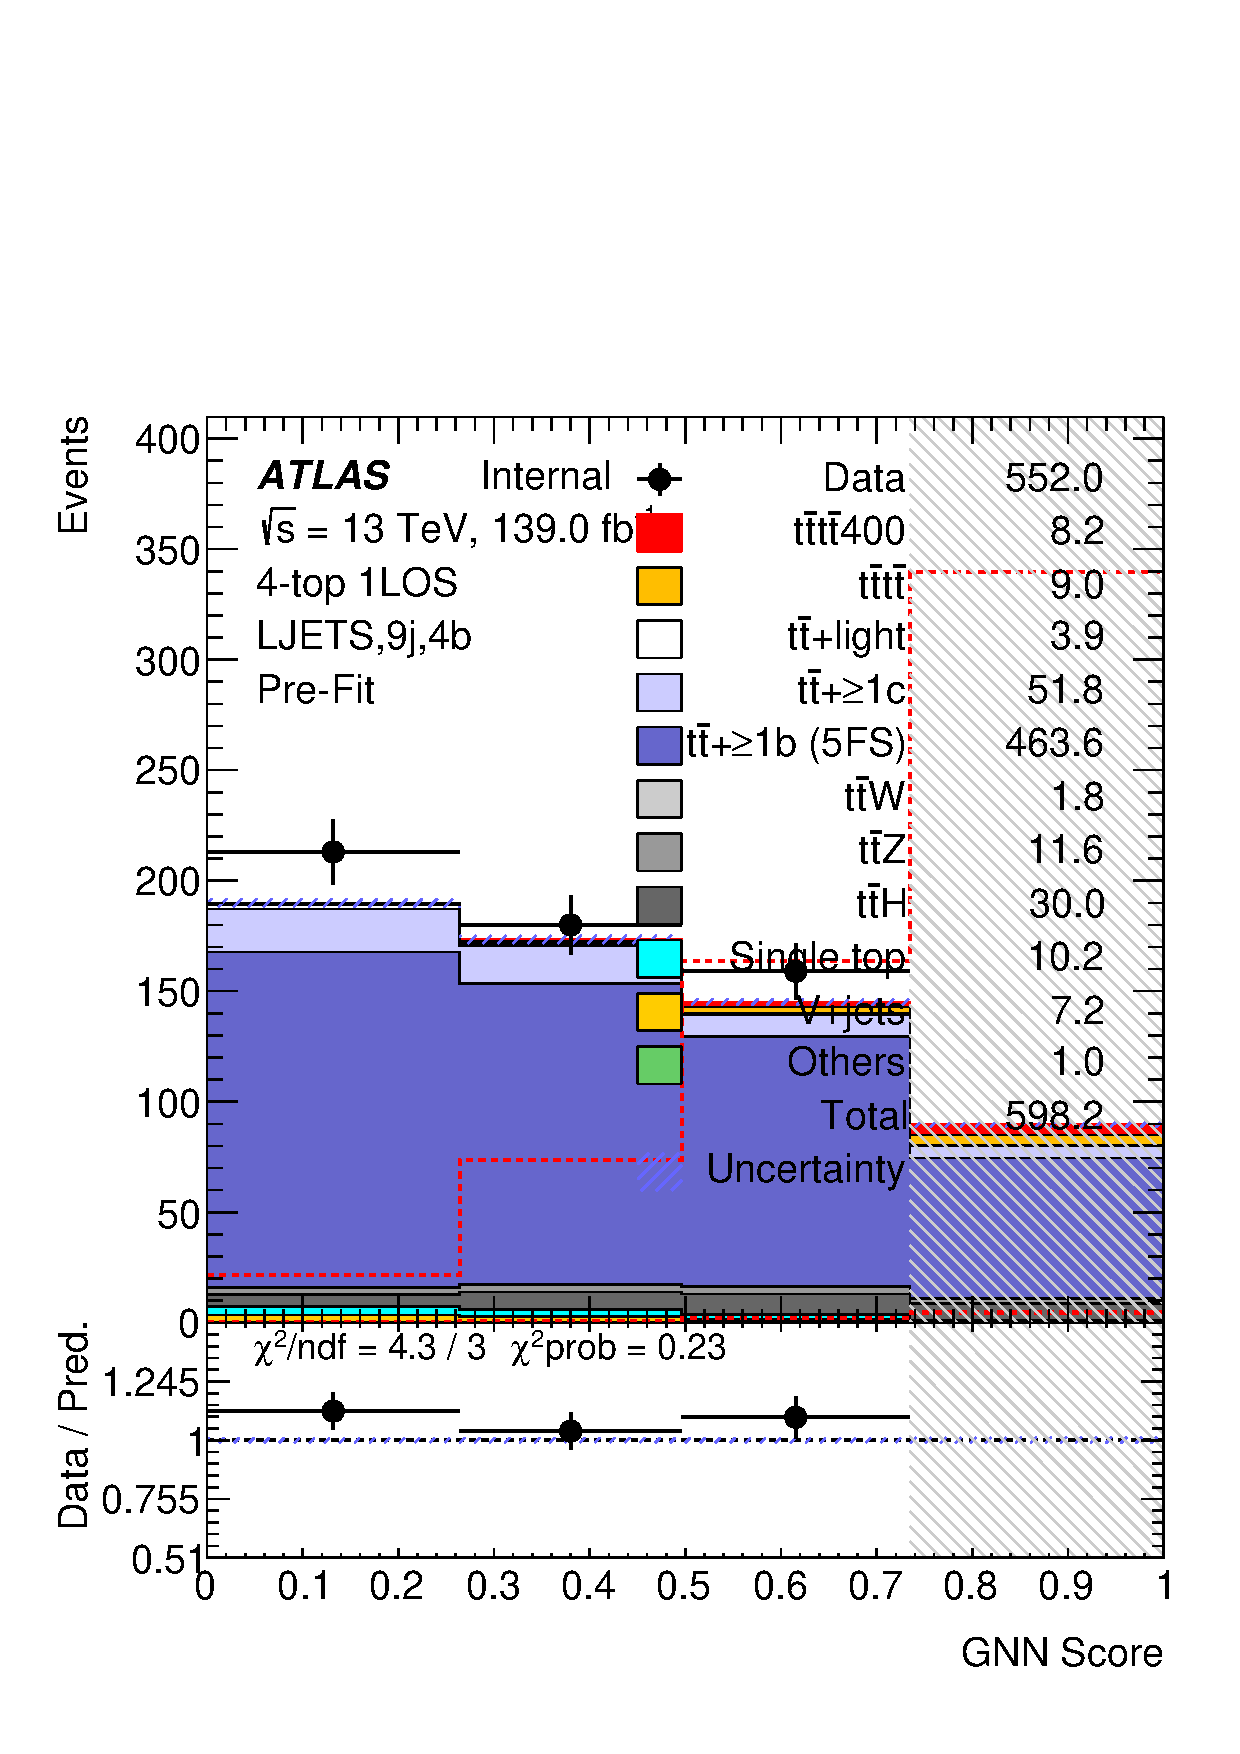
\includegraphics[width=0.25 \textwidth]{figures/fits/4FSvs5FS/GNN/400/Data_to_MC_5FS/ljets_9j4b.pdf} &                                                                    
        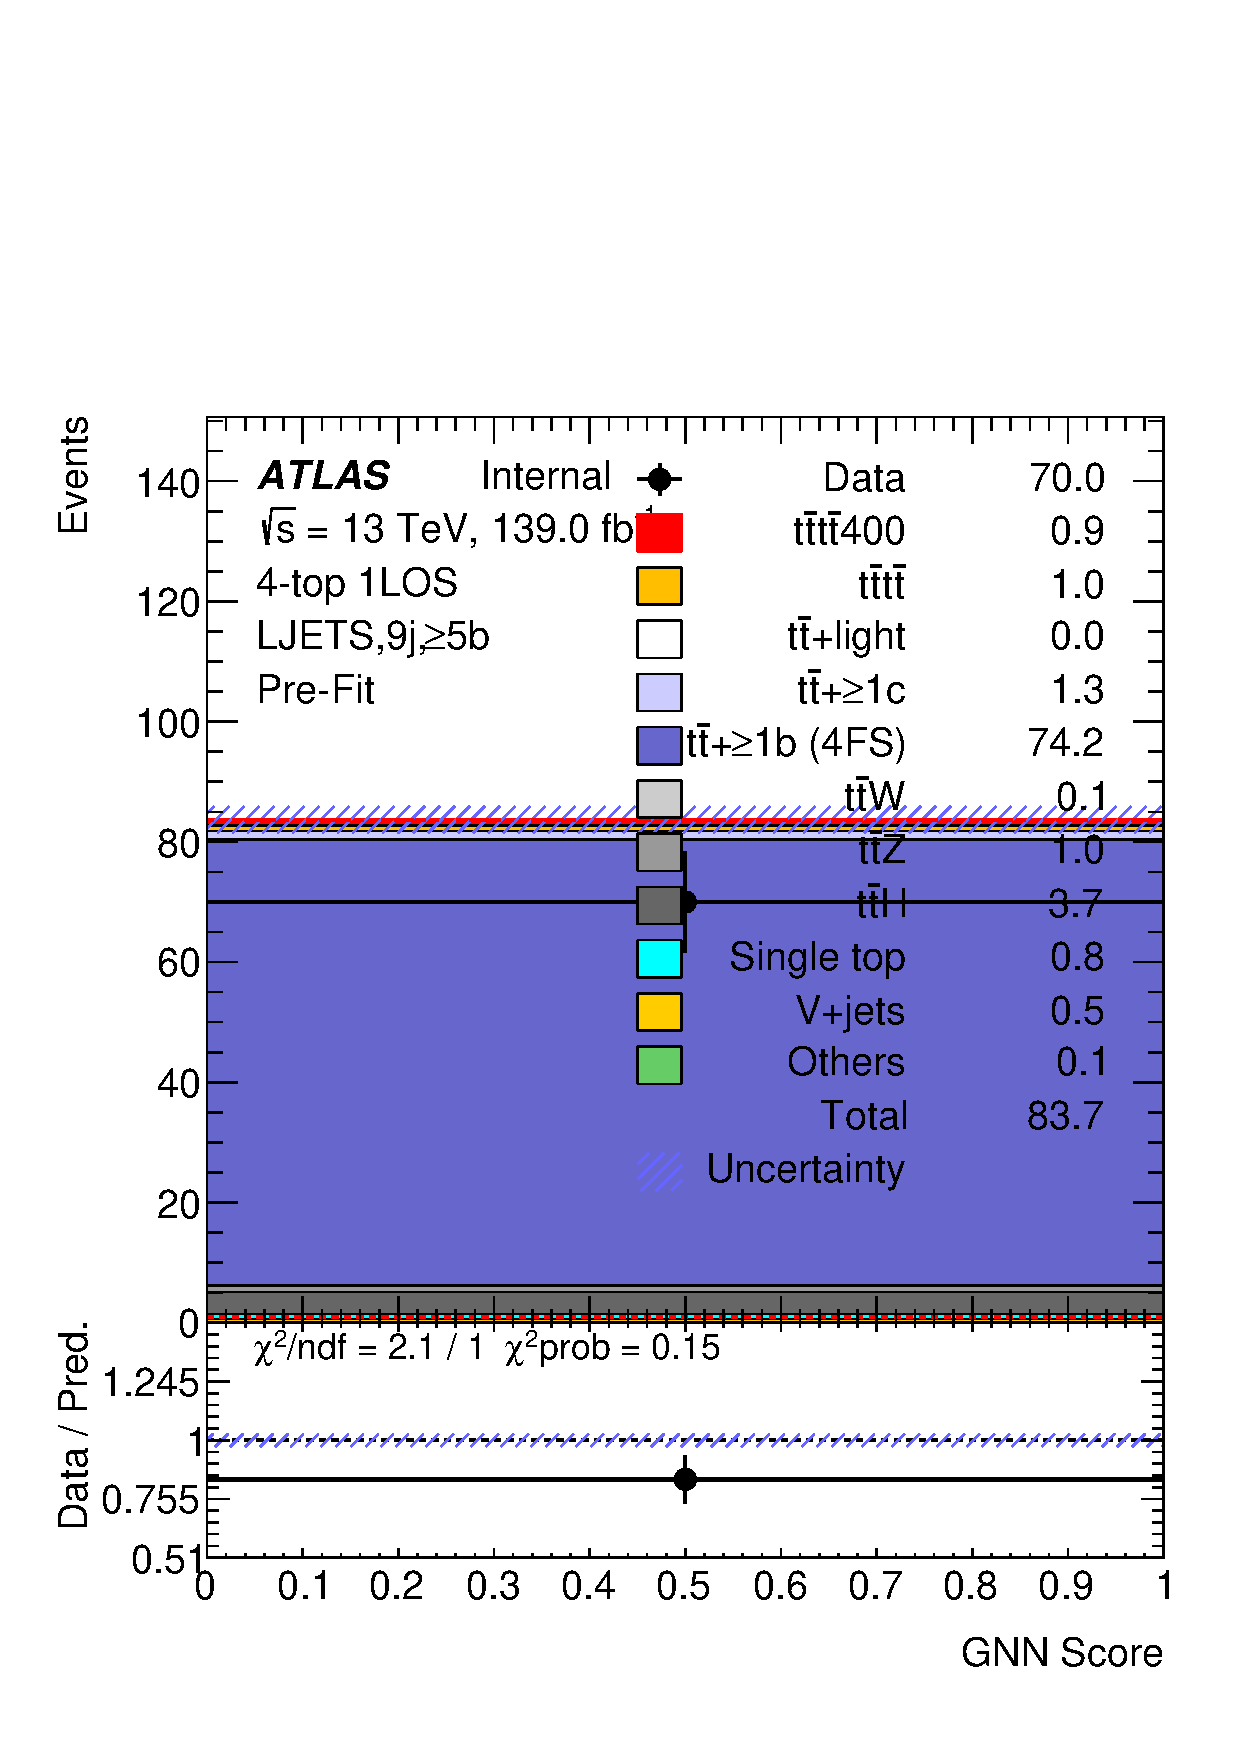
\includegraphics[width=0.25 \textwidth]{figures/fits/4FSvs5FS/GNN/400/Data_to_MC_4FS/ljets_9jge5b.pdf} &                                                                 
        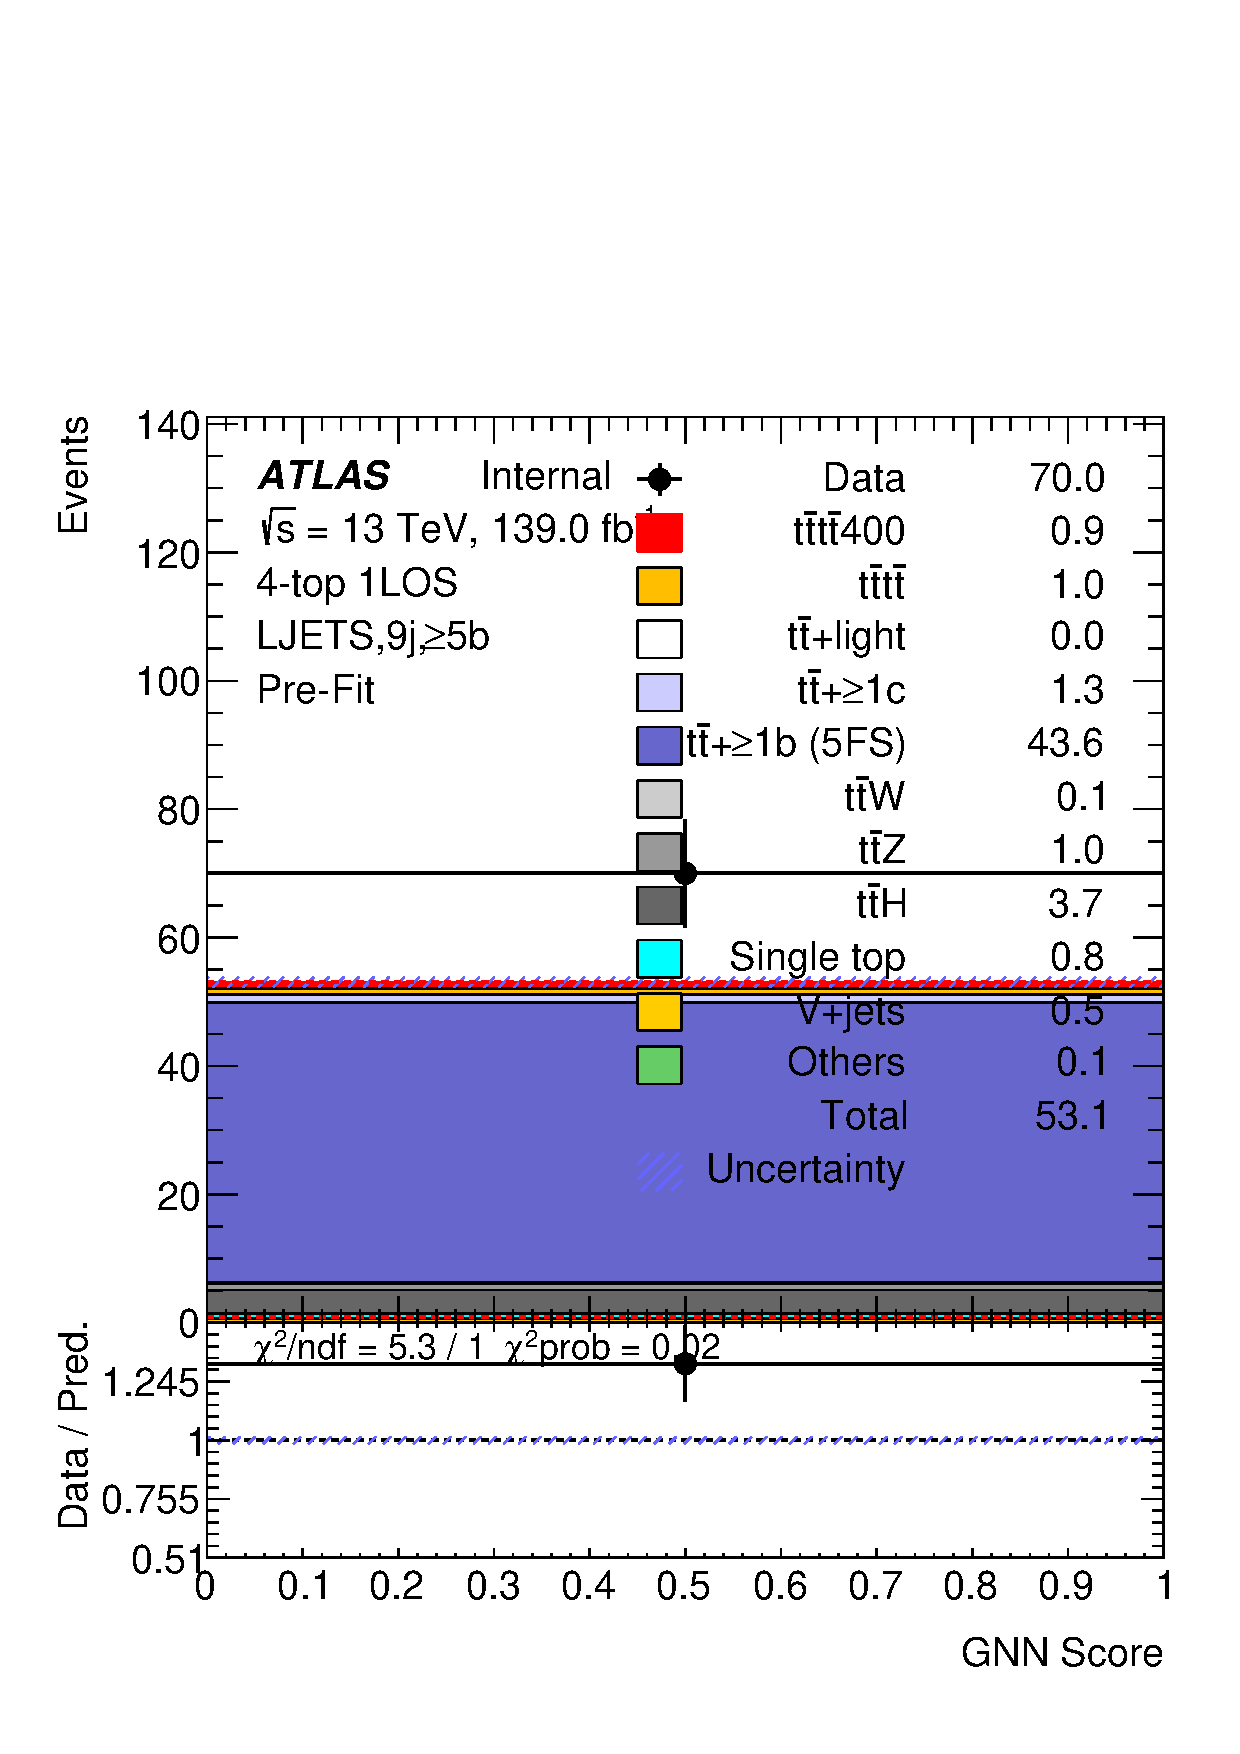
\includegraphics[width=0.25 \textwidth]{figures/fits/4FSvs5FS/GNN/400/Data_to_MC_5FS/ljets_9jge5b.pdf} \\                                                                
  
        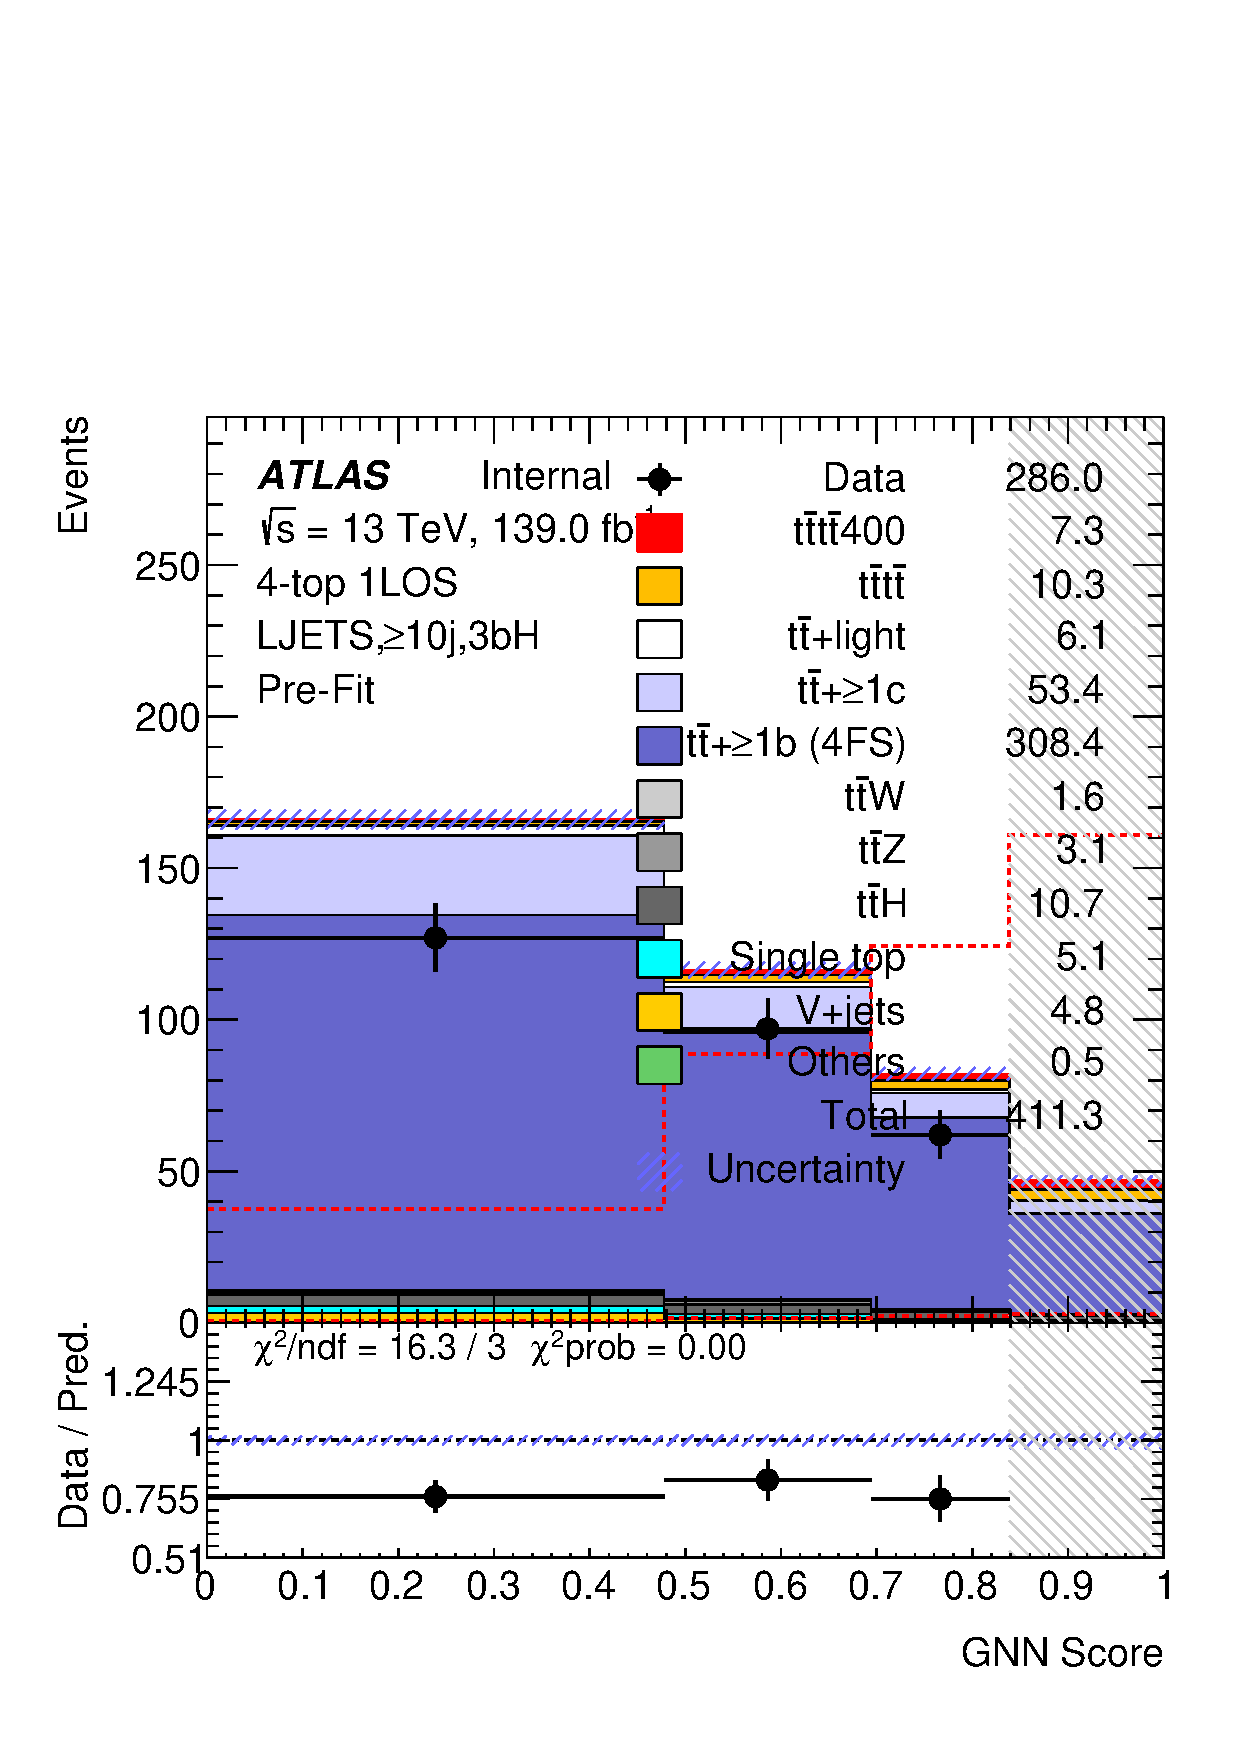
\includegraphics[width=0.25 \textwidth]{figures/fits/4FSvs5FS/GNN/400/Data_to_MC_4FS/ljets_ge10j3bH.pdf} &                                                                 
        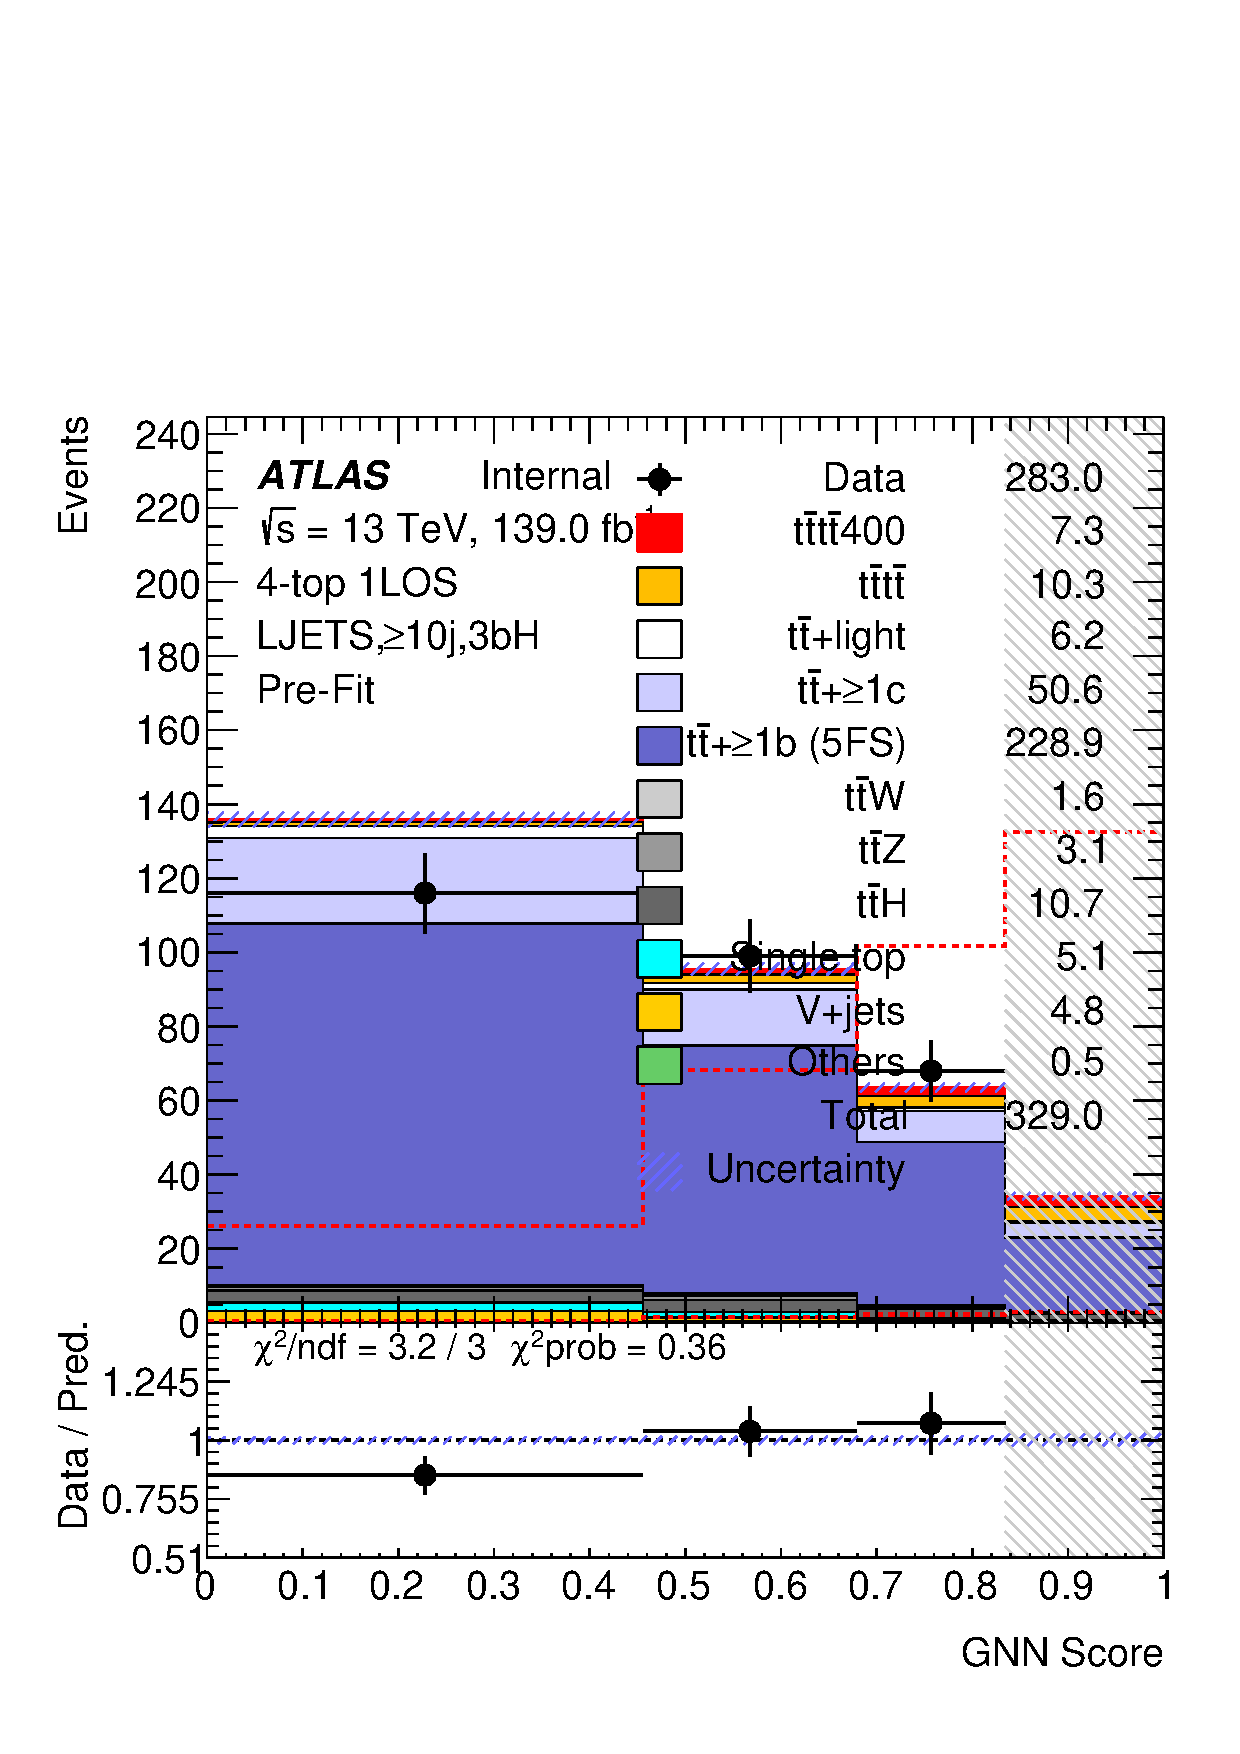
\includegraphics[width=0.25 \textwidth]{figures/fits/4FSvs5FS/GNN/400/Data_to_MC_5FS/ljets_ge10j3bH.pdf} &                                                                 
        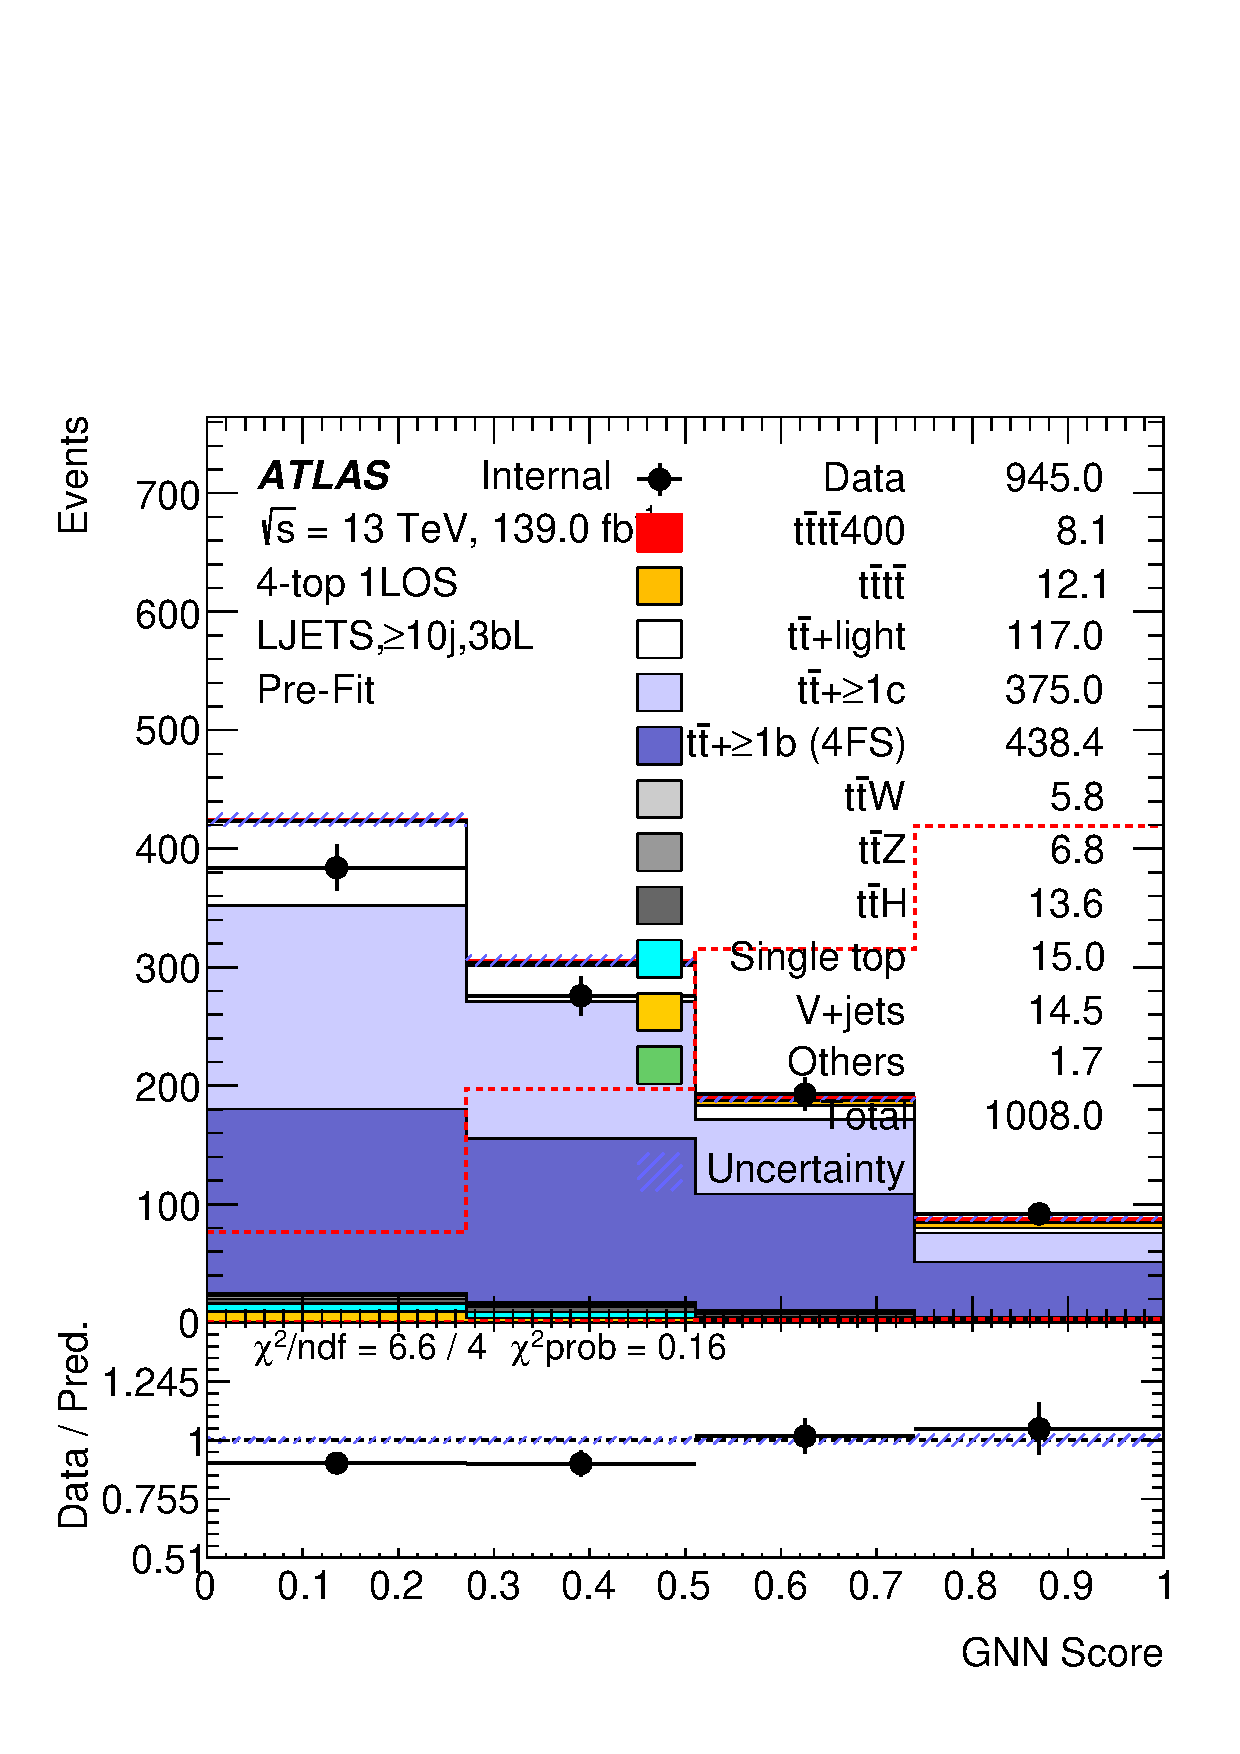
\includegraphics[width=0.25 \textwidth]{figures/fits/4FSvs5FS/GNN/400/Data_to_MC_4FS/ljets_ge10j3bL.pdf} &                                                                
        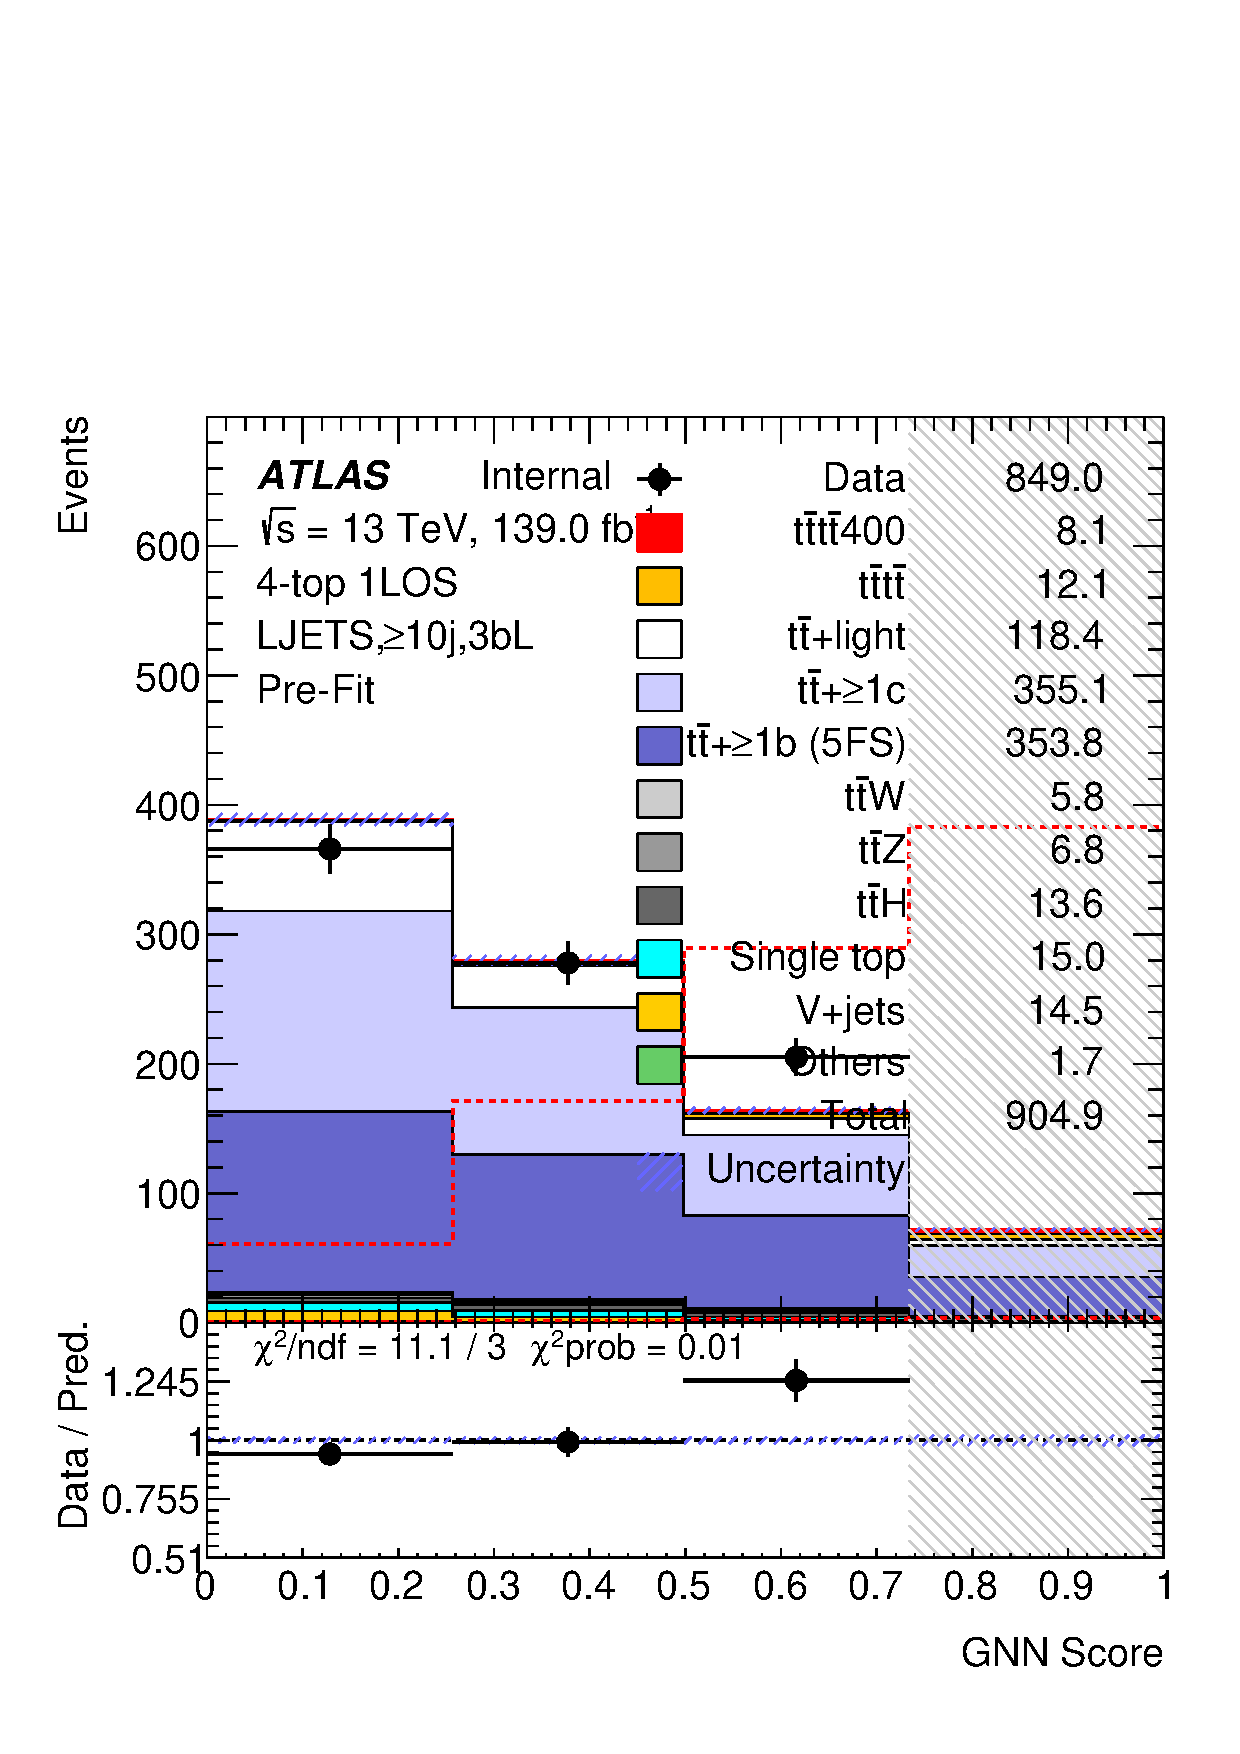
\includegraphics[width=0.25 \textwidth]{figures/fits/4FSvs5FS/GNN/400/Data_to_MC_5FS/ljets_ge10j3bL.pdf}\\    
                                                                                                                                                                       
        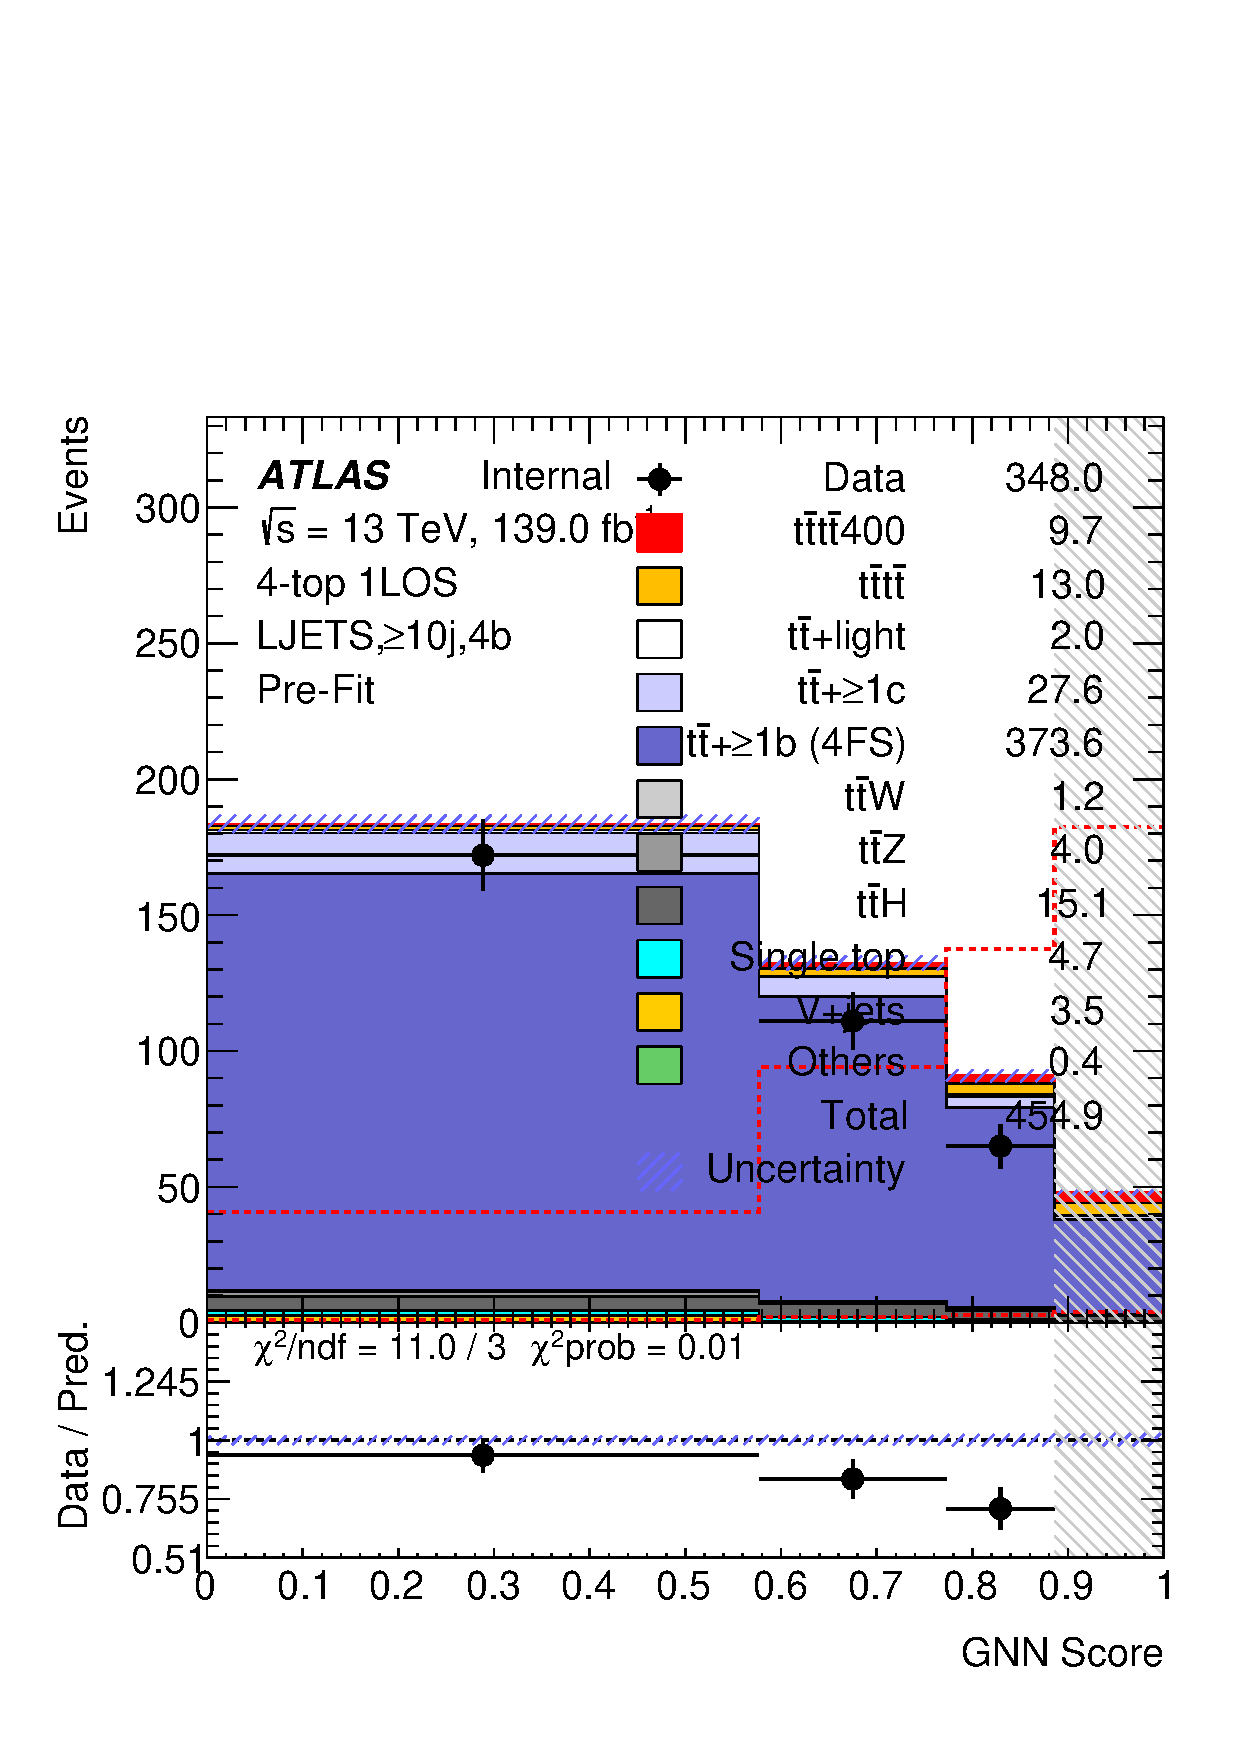
\includegraphics[width=0.25 \textwidth]{figures/fits/4FSvs5FS/GNN/400/Data_to_MC_4FS/ljets_ge10j4b.pdf} &                                                                  
        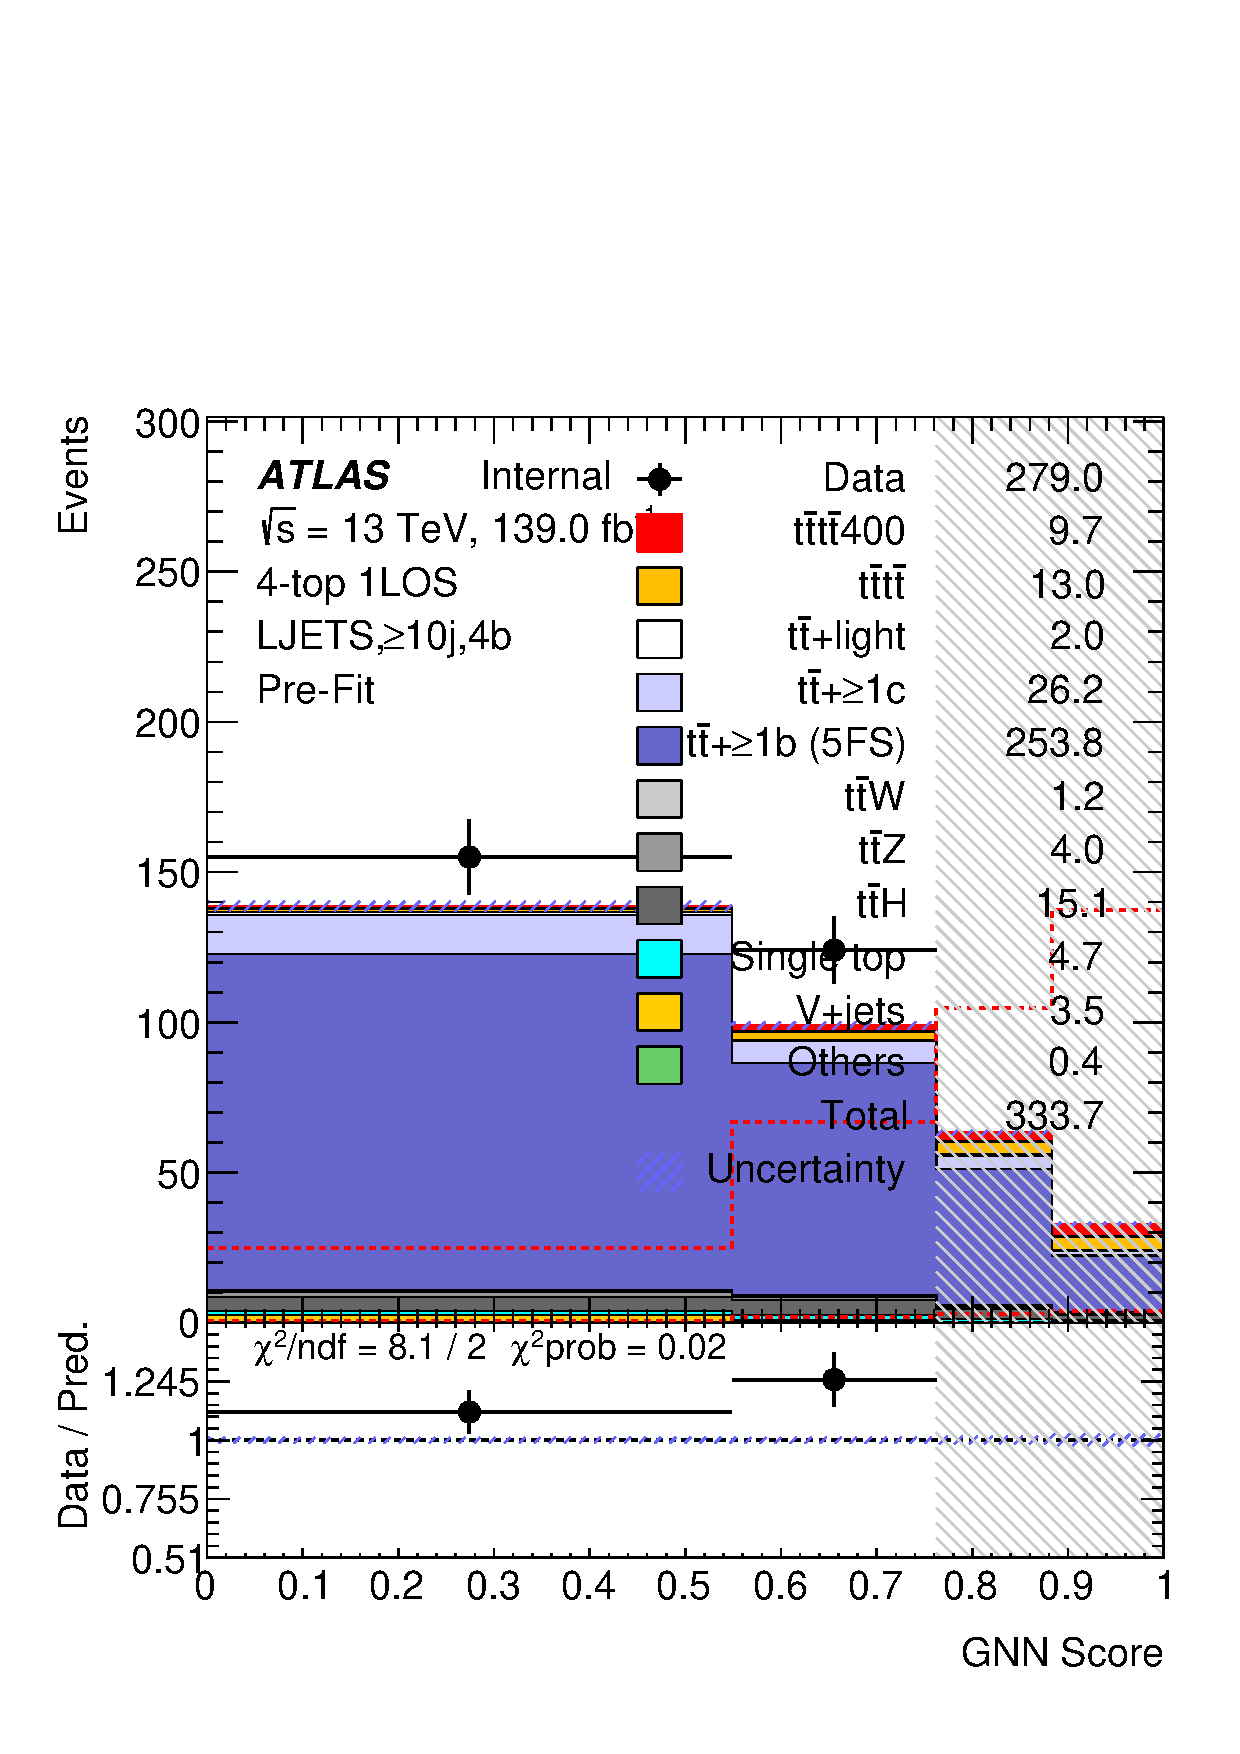
\includegraphics[width=0.25 \textwidth]{figures/fits/4FSvs5FS/GNN/400/Data_to_MC_5FS/ljets_ge10j4b.pdf} &                                                                  
        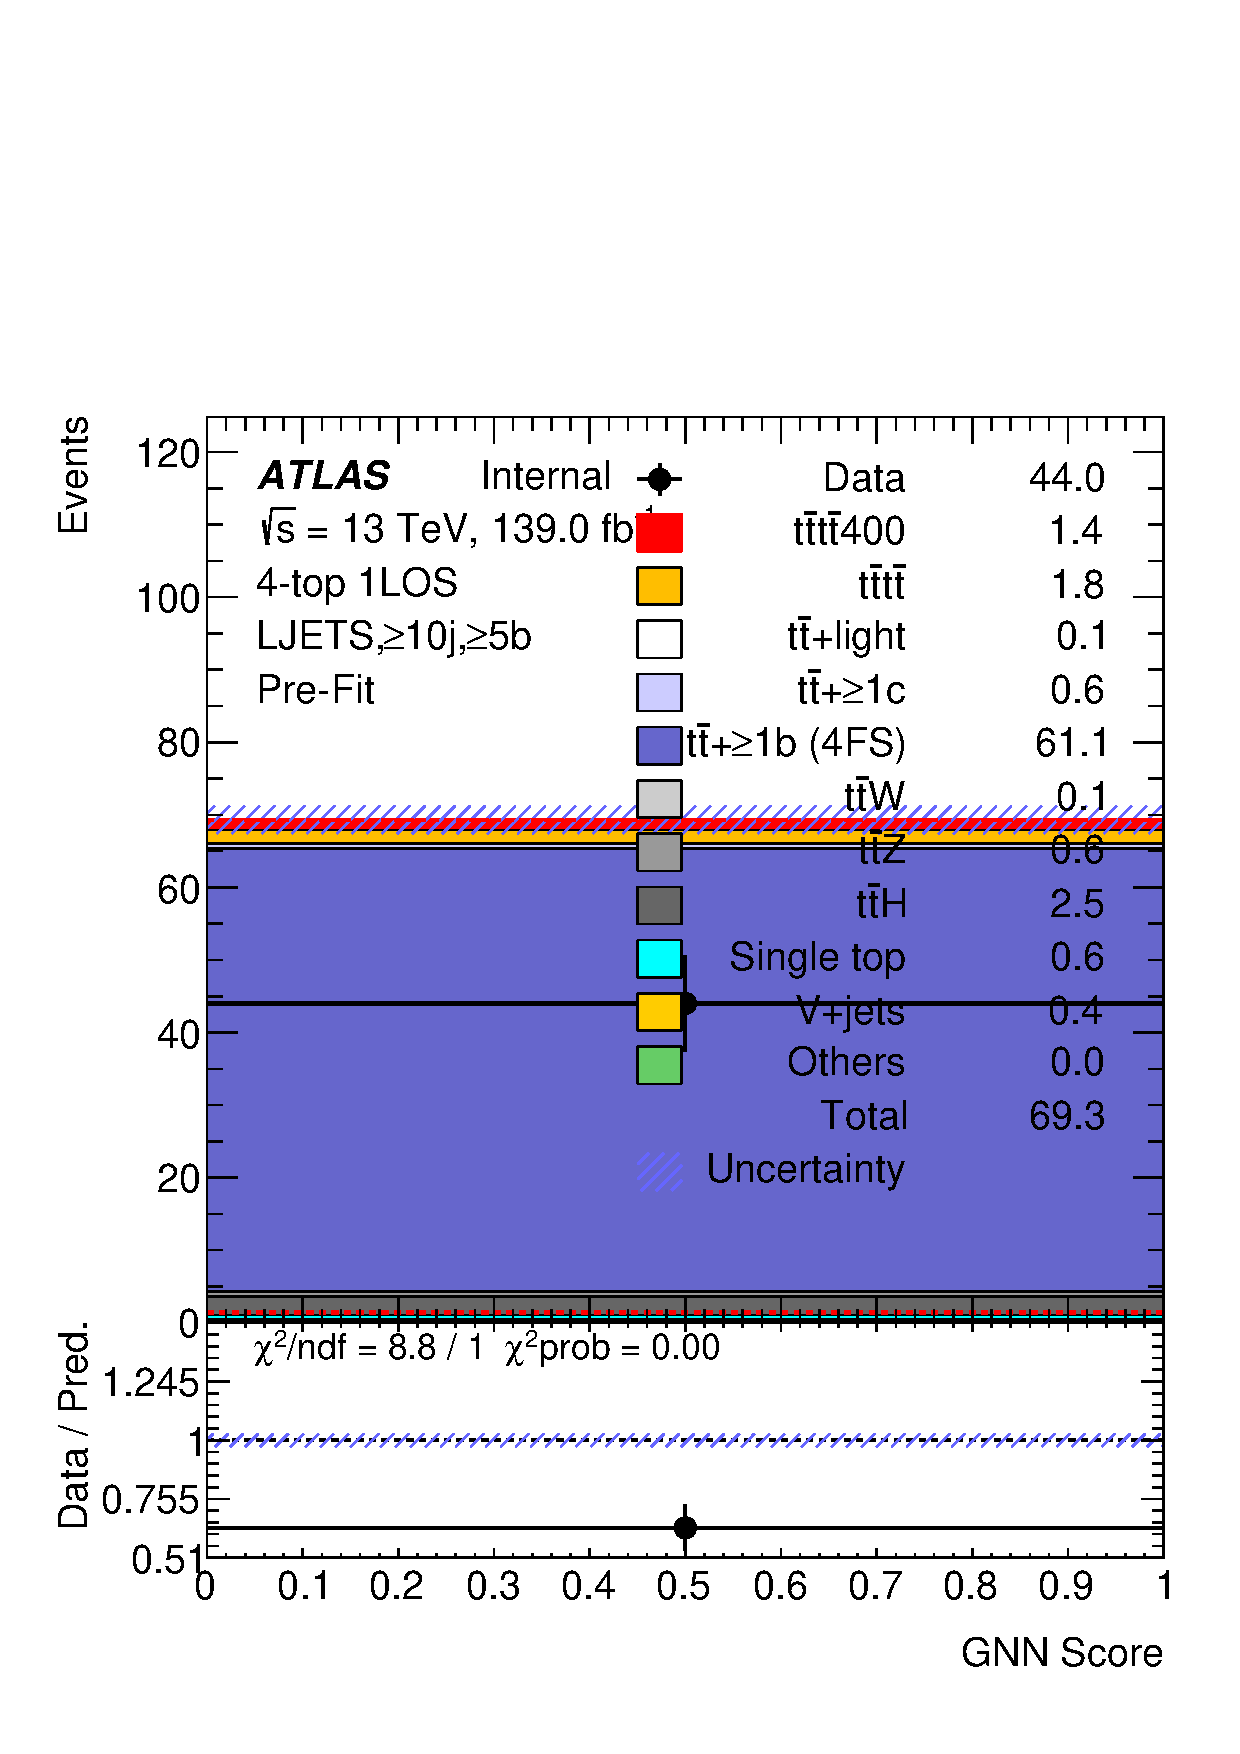
\includegraphics[width=0.25 \textwidth]{figures/fits/4FSvs5FS/GNN/400/Data_to_MC_4FS/ljets_ge10jge5b.pdf} &                                                                
        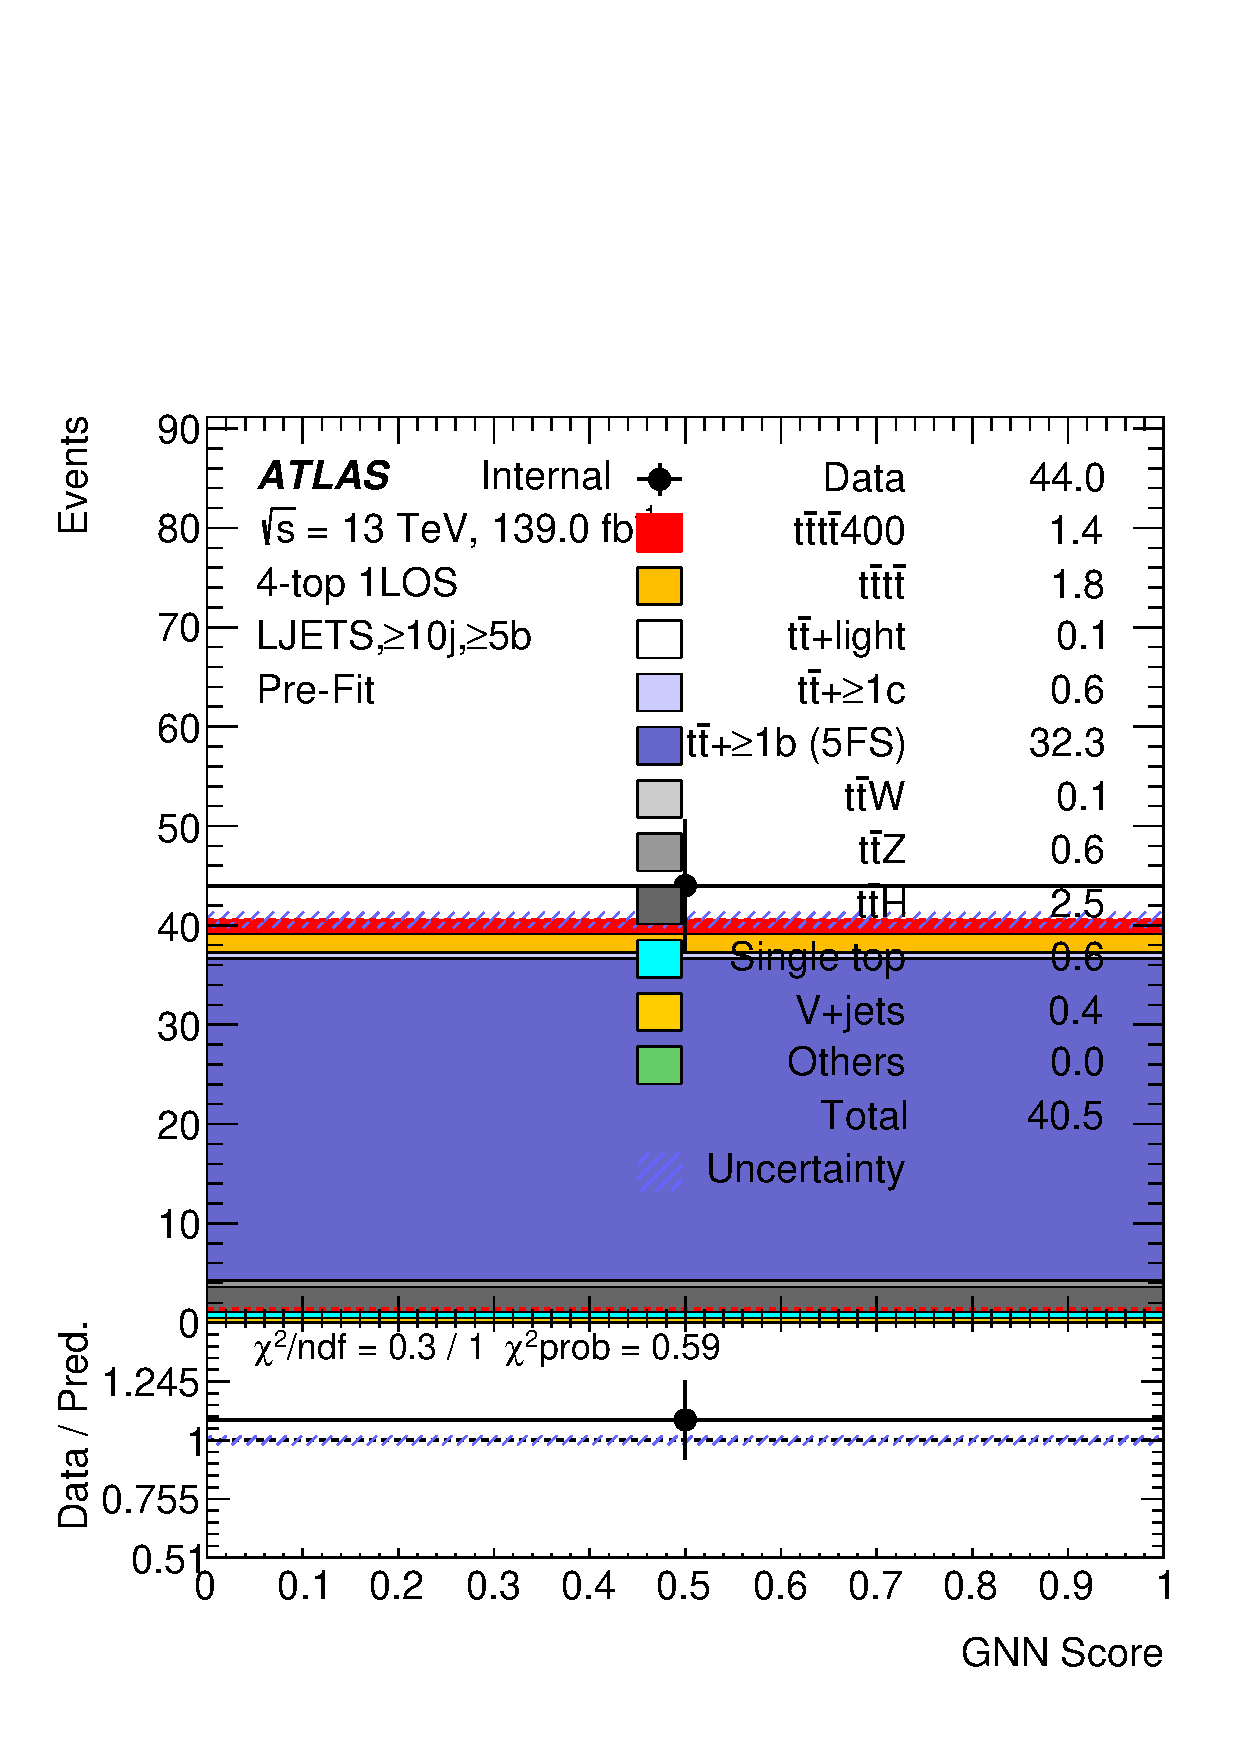
\includegraphics[width=0.25 \textwidth]{figures/fits/4FSvs5FS/GNN/400/Data_to_MC_5FS/ljets_ge10jge5b.pdf} \\                                                               
        \end{tabular}                                                                                                                                                              
        \caption{\label{4FSvs5FS_dataMC_1L}Pre-fit distributions in 5FS compared with 4FS for 1L channel associated with different signal and background samples, compared with data yields.}                                                                                                                                           
\end{center}                                                                                                                                                                      
\end{figure}          


\begin{figure}[htbp!]                                                                                                                                                       
  \begin{center} \setlength{\tabcolsep}{2.5pt}\footnotesize                                                                                                                  
    \begin{tabular}{cccc}                                                                                                                                                    
      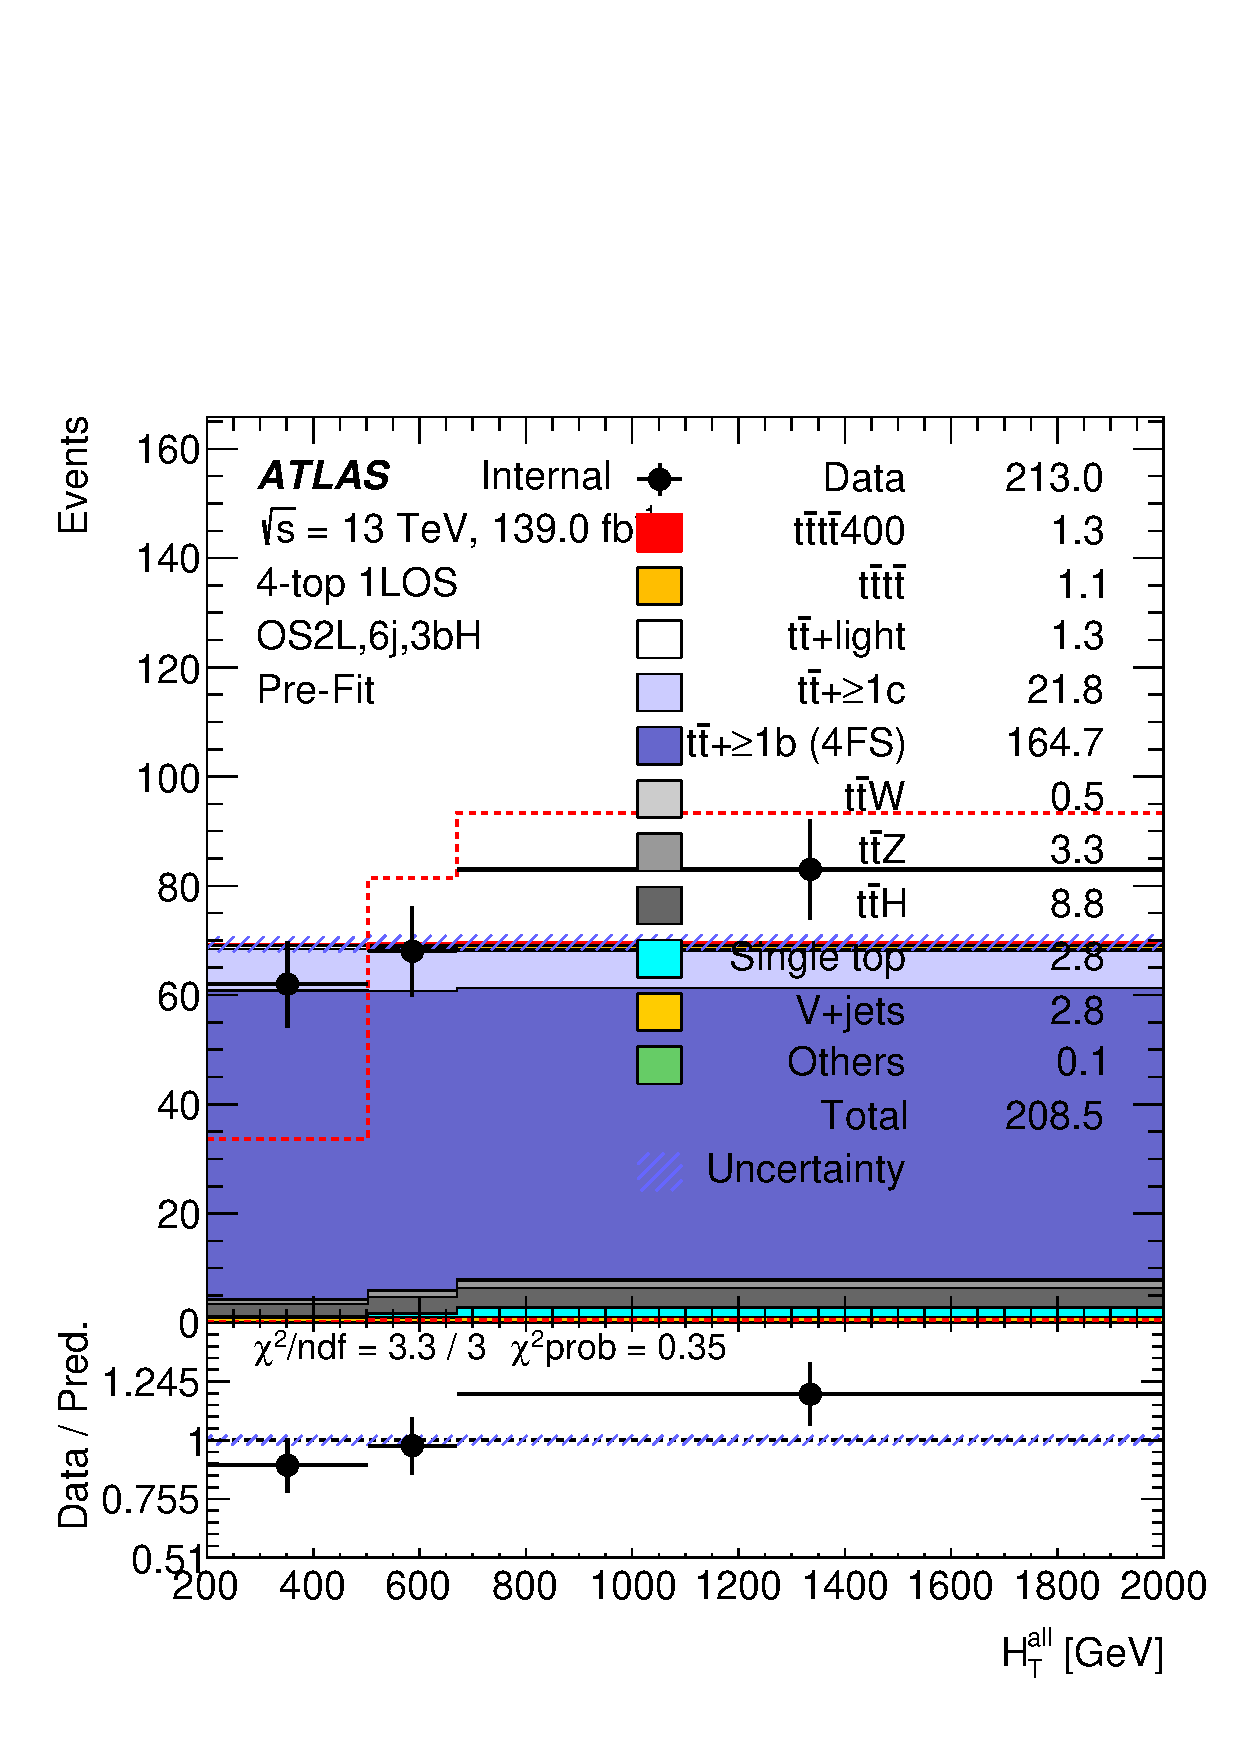
\includegraphics[width=0.23 \textwidth]{figures/fits/4FSvs5FS/GNN/400/Data_to_MC_4FS/os2l_6j3bH.pdf} &                                                                      
      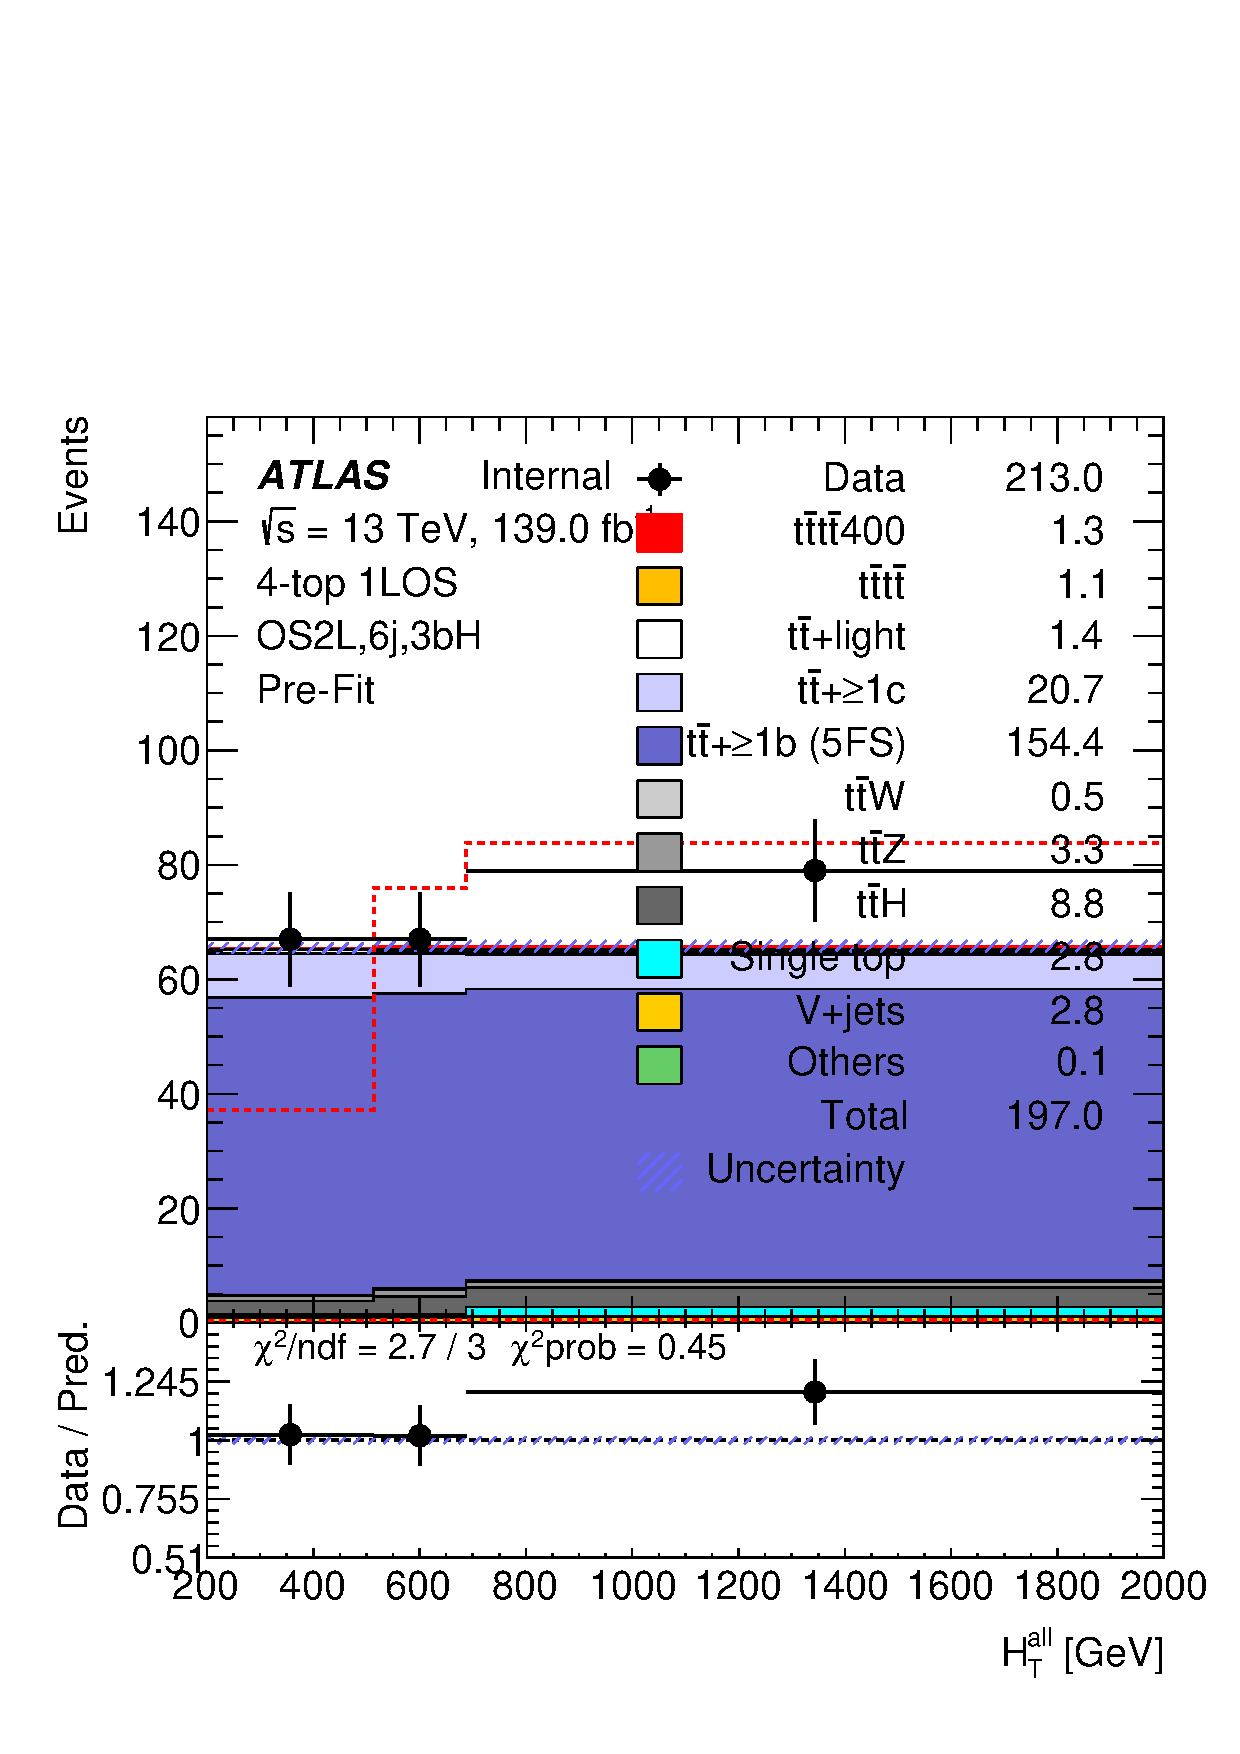
\includegraphics[width=0.23 \textwidth]{figures/fits/4FSvs5FS/GNN/400/Data_to_MC_5FS/os2l_6j3bH.pdf} &                                                                      
      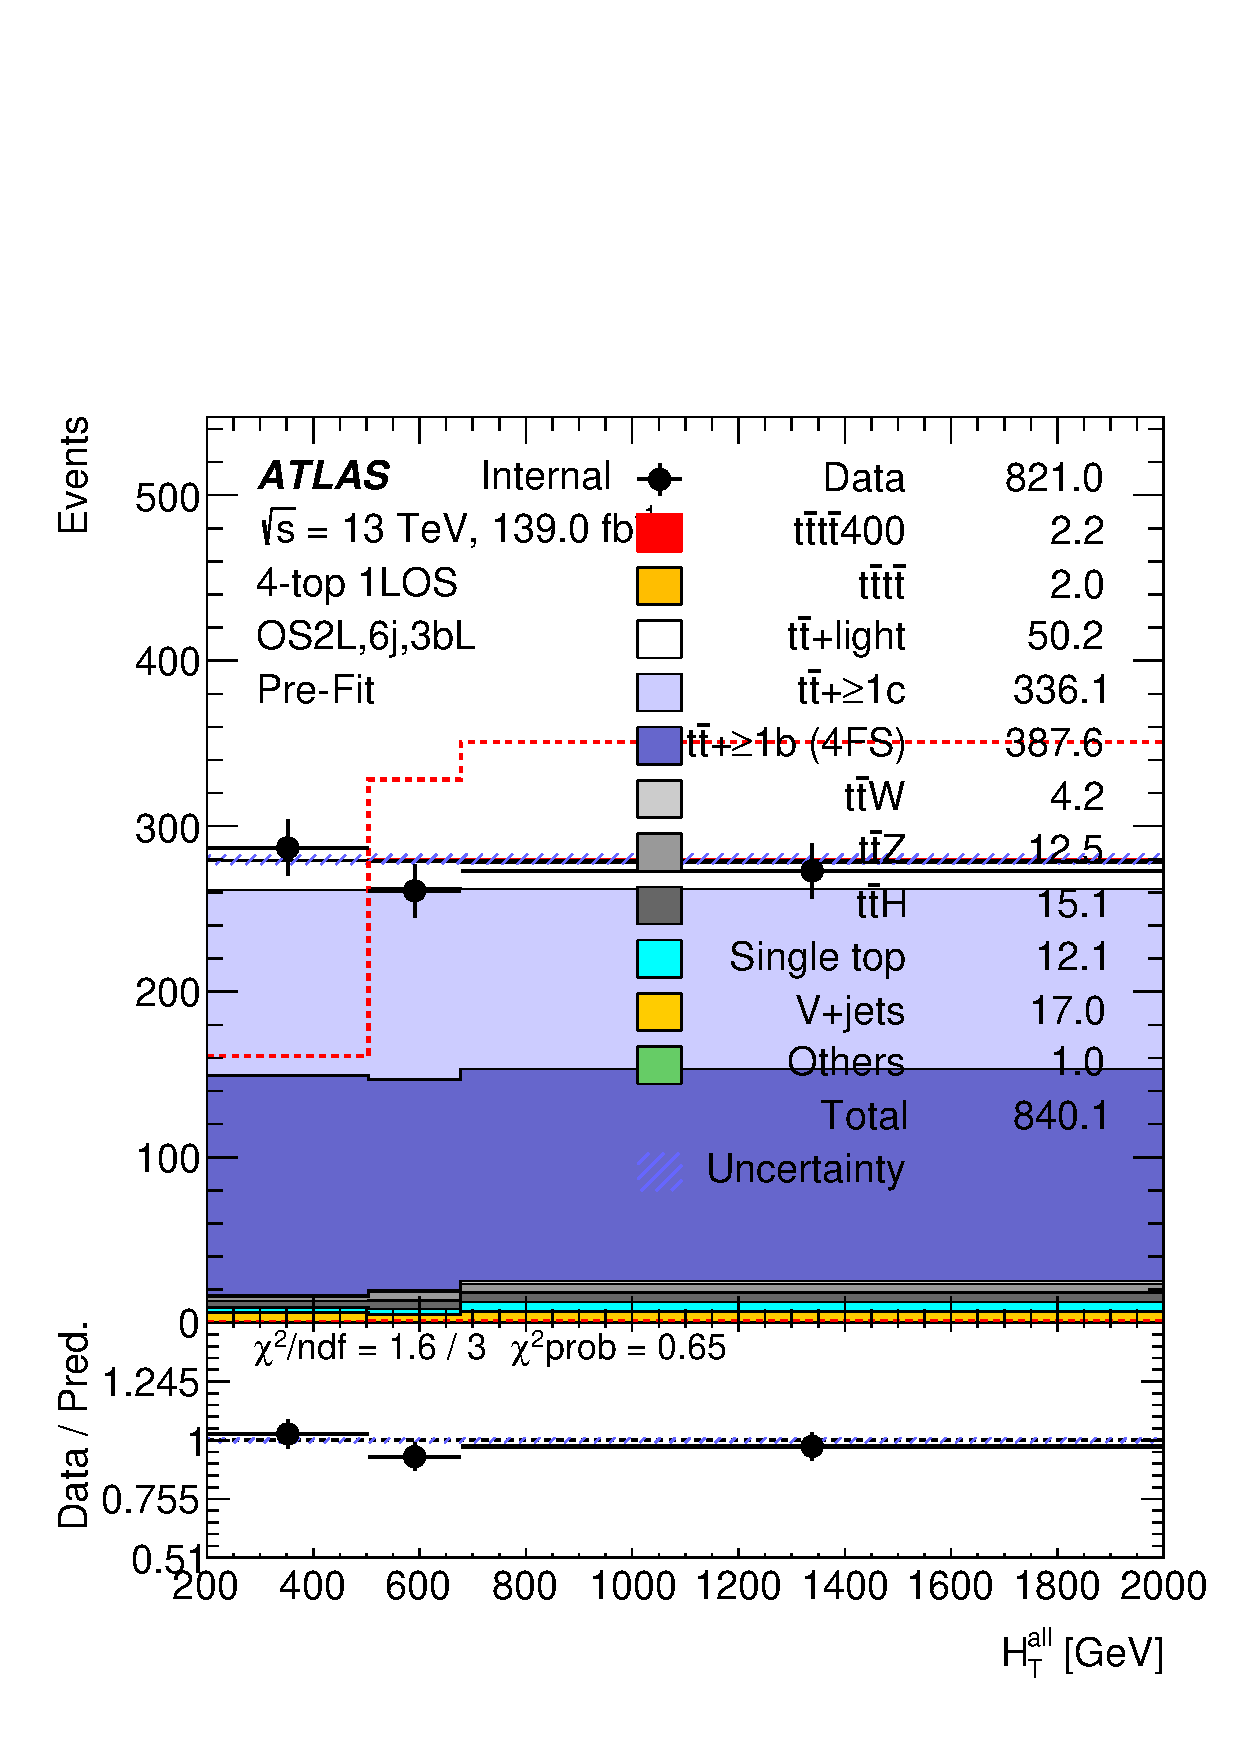
\includegraphics[width=0.23 \textwidth]{figures/fits/4FSvs5FS/GNN/400/Data_to_MC_4FS/os2l_6j3bL.pdf} &                                                                      
      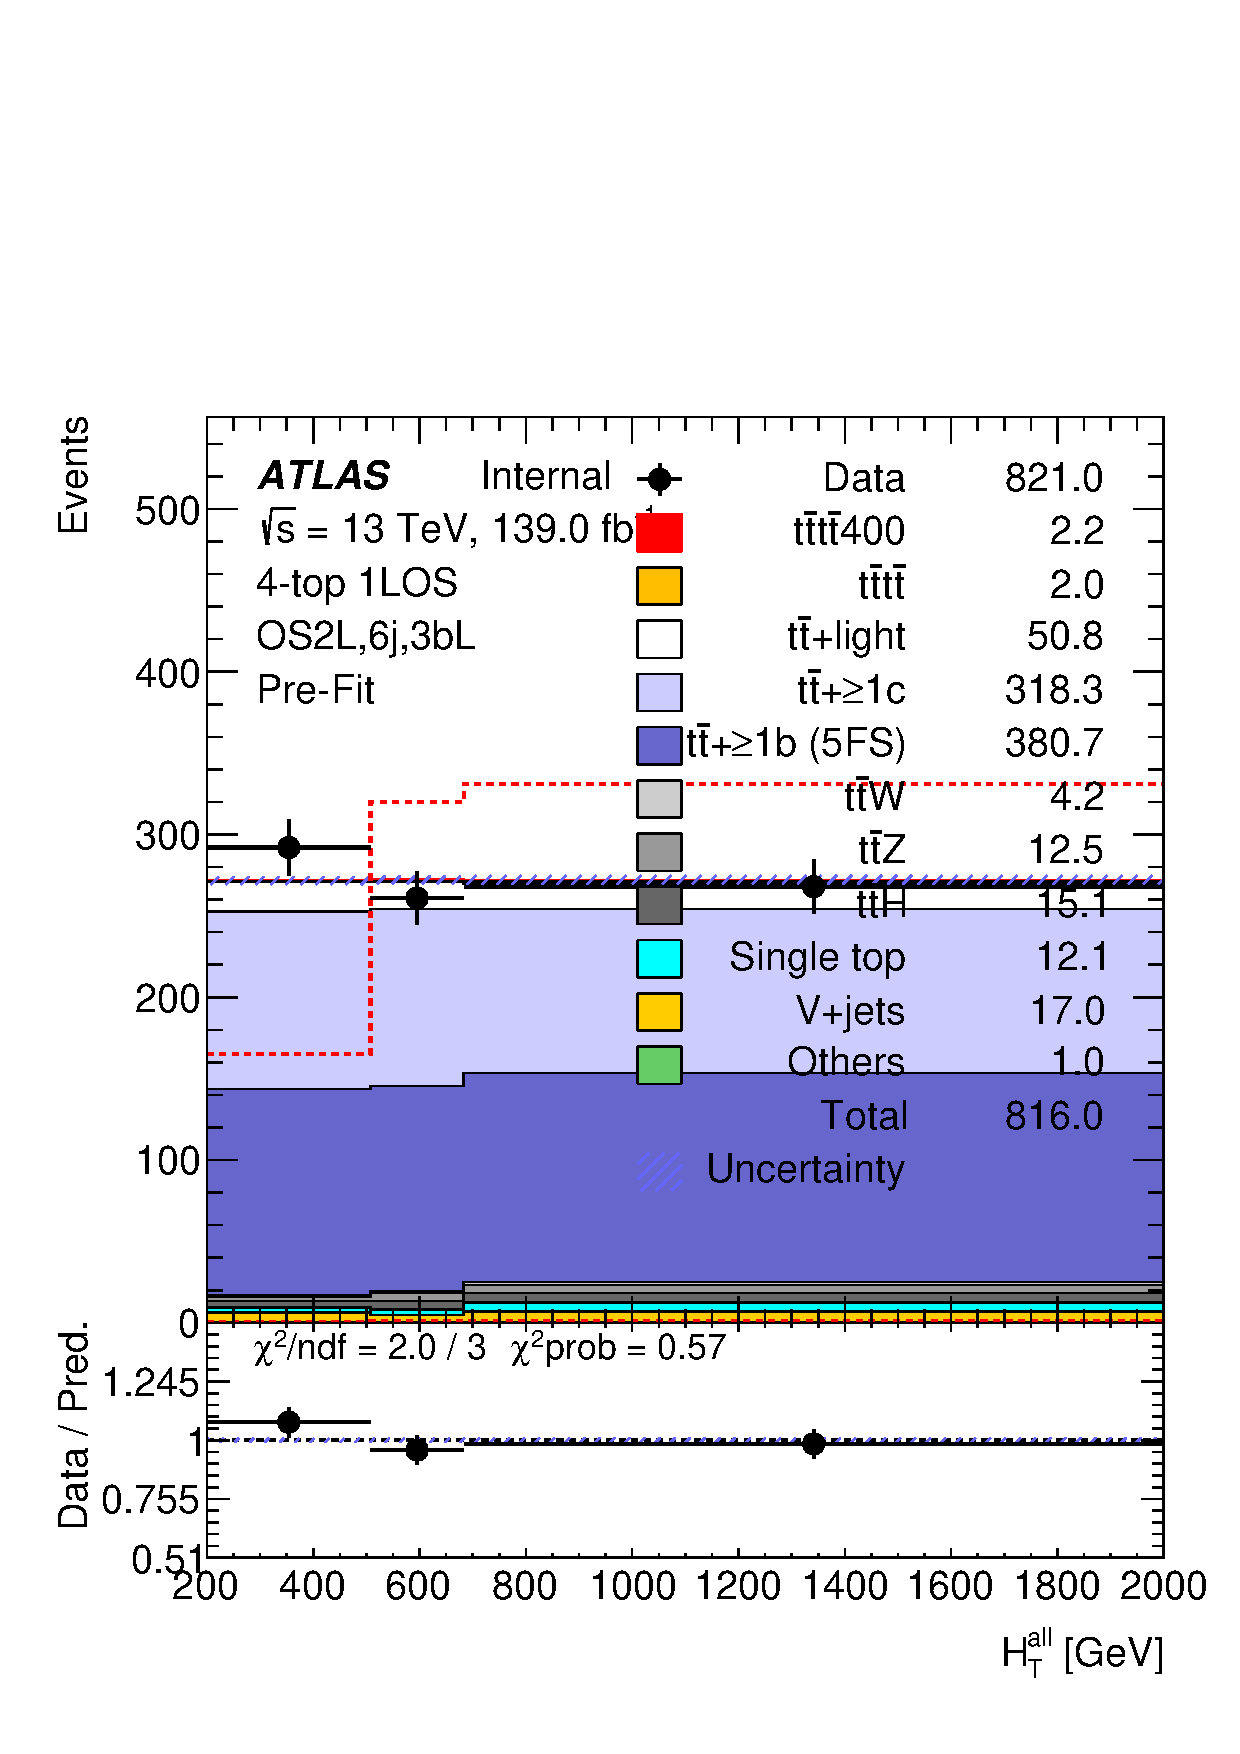
\includegraphics[width=0.23 \textwidth]{figures/fits/4FSvs5FS/GNN/400/Data_to_MC_5FS/os2l_6j3bL.pdf}\\                                                                    
      
      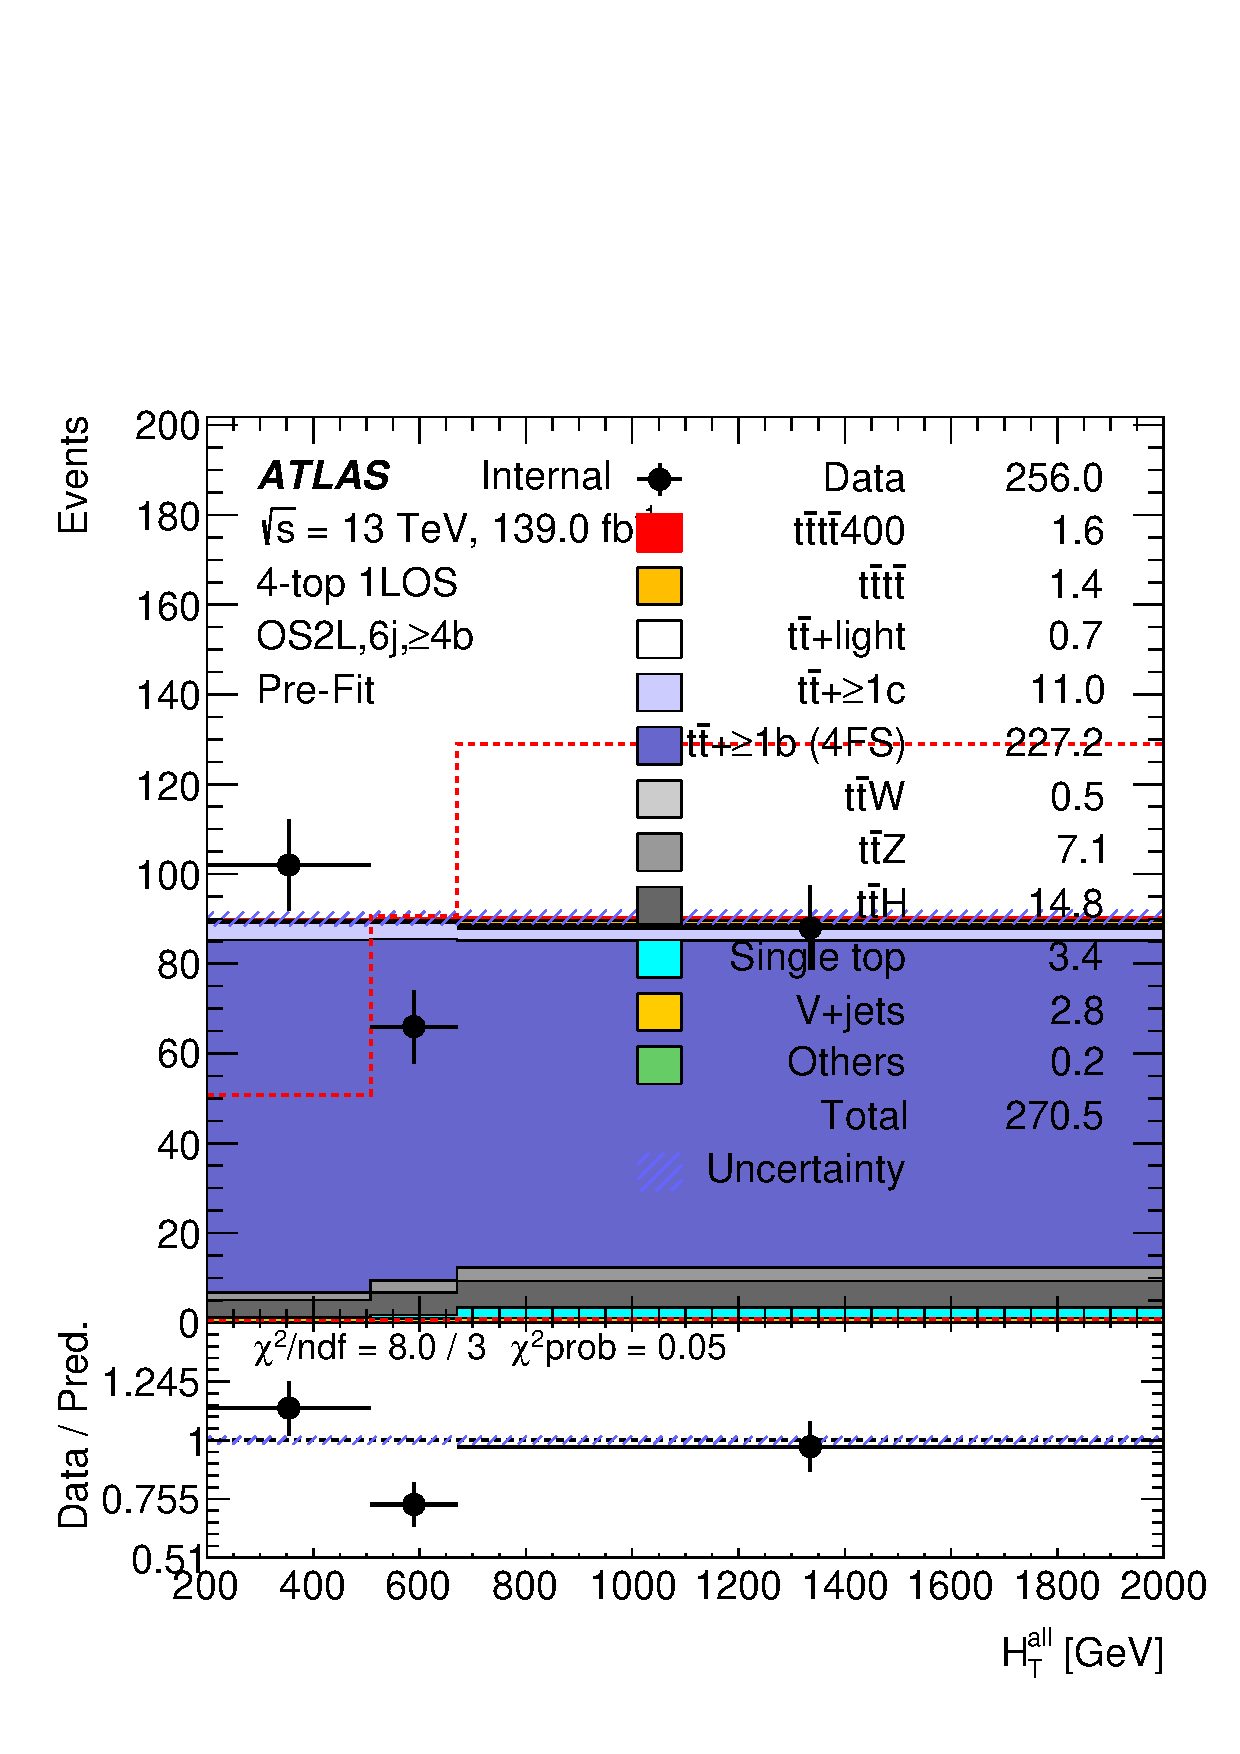
\includegraphics[width=0.23 \textwidth]{figures/fits/4FSvs5FS/GNN/400/Data_to_MC_4FS/os2l_6jge4b.pdf} &                                                                      
      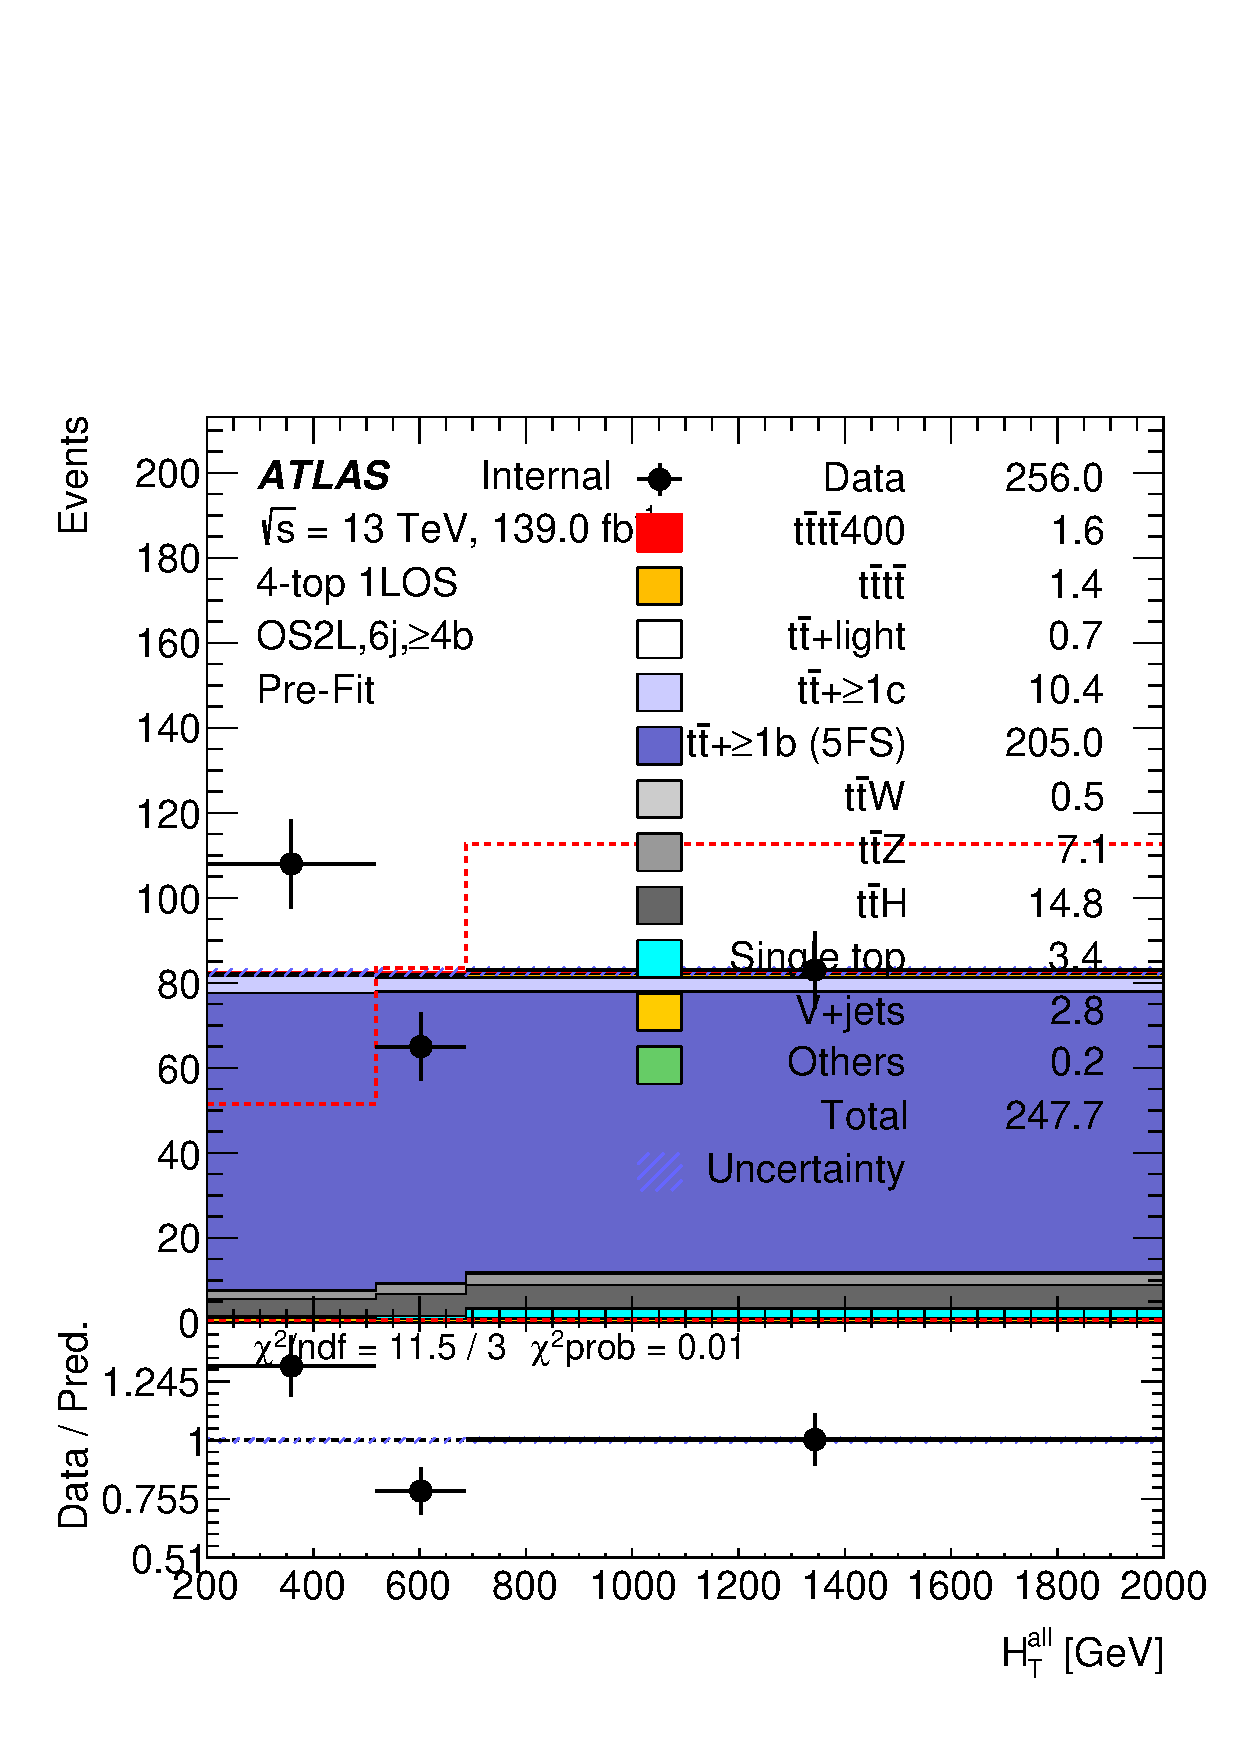
\includegraphics[width=0.23 \textwidth]{figures/fits/4FSvs5FS/GNN/400/Data_to_MC_5FS/os2l_6jge4b.pdf} &                                                                      
      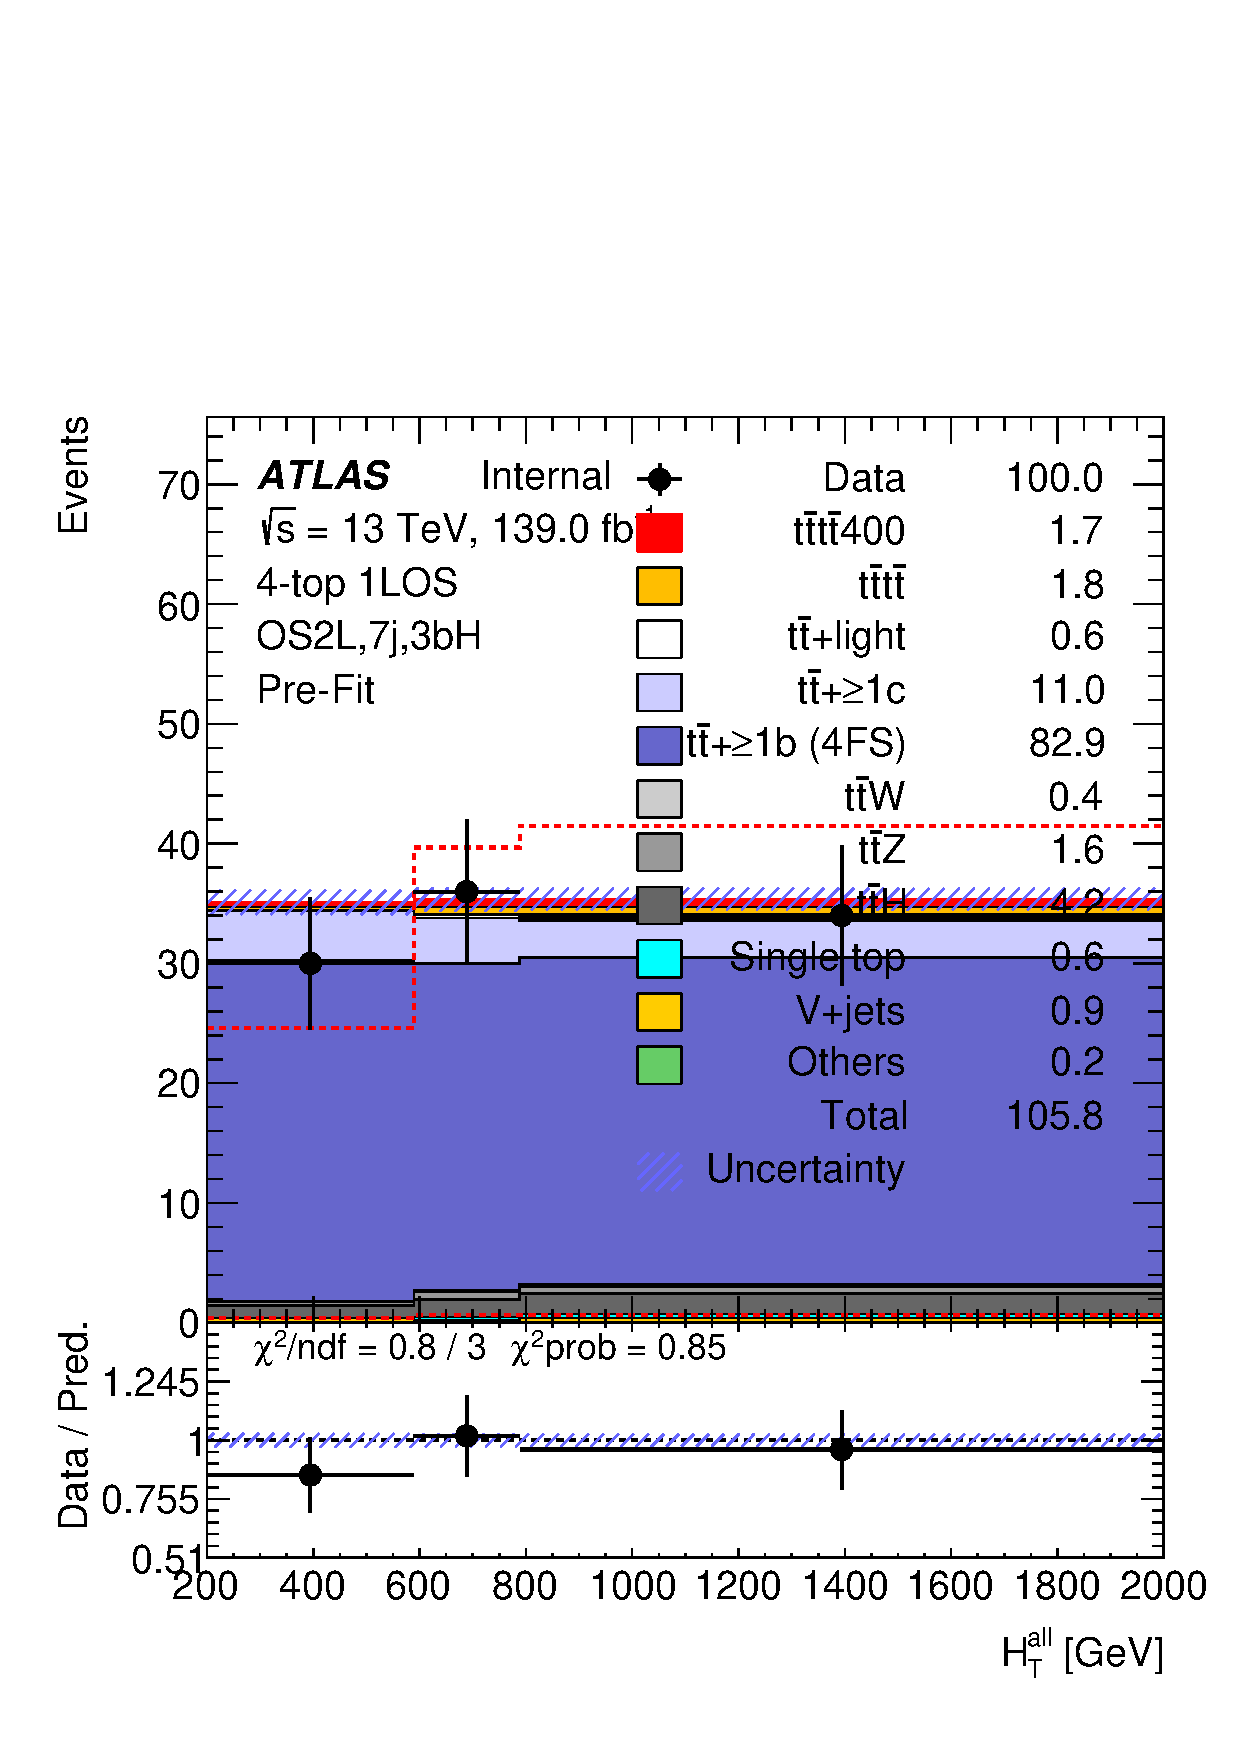
\includegraphics[width=0.23 \textwidth]{figures/fits/4FSvs5FS/GNN/400/Data_to_MC_4FS/os2l_7j3bH.pdf} &                                                                     
      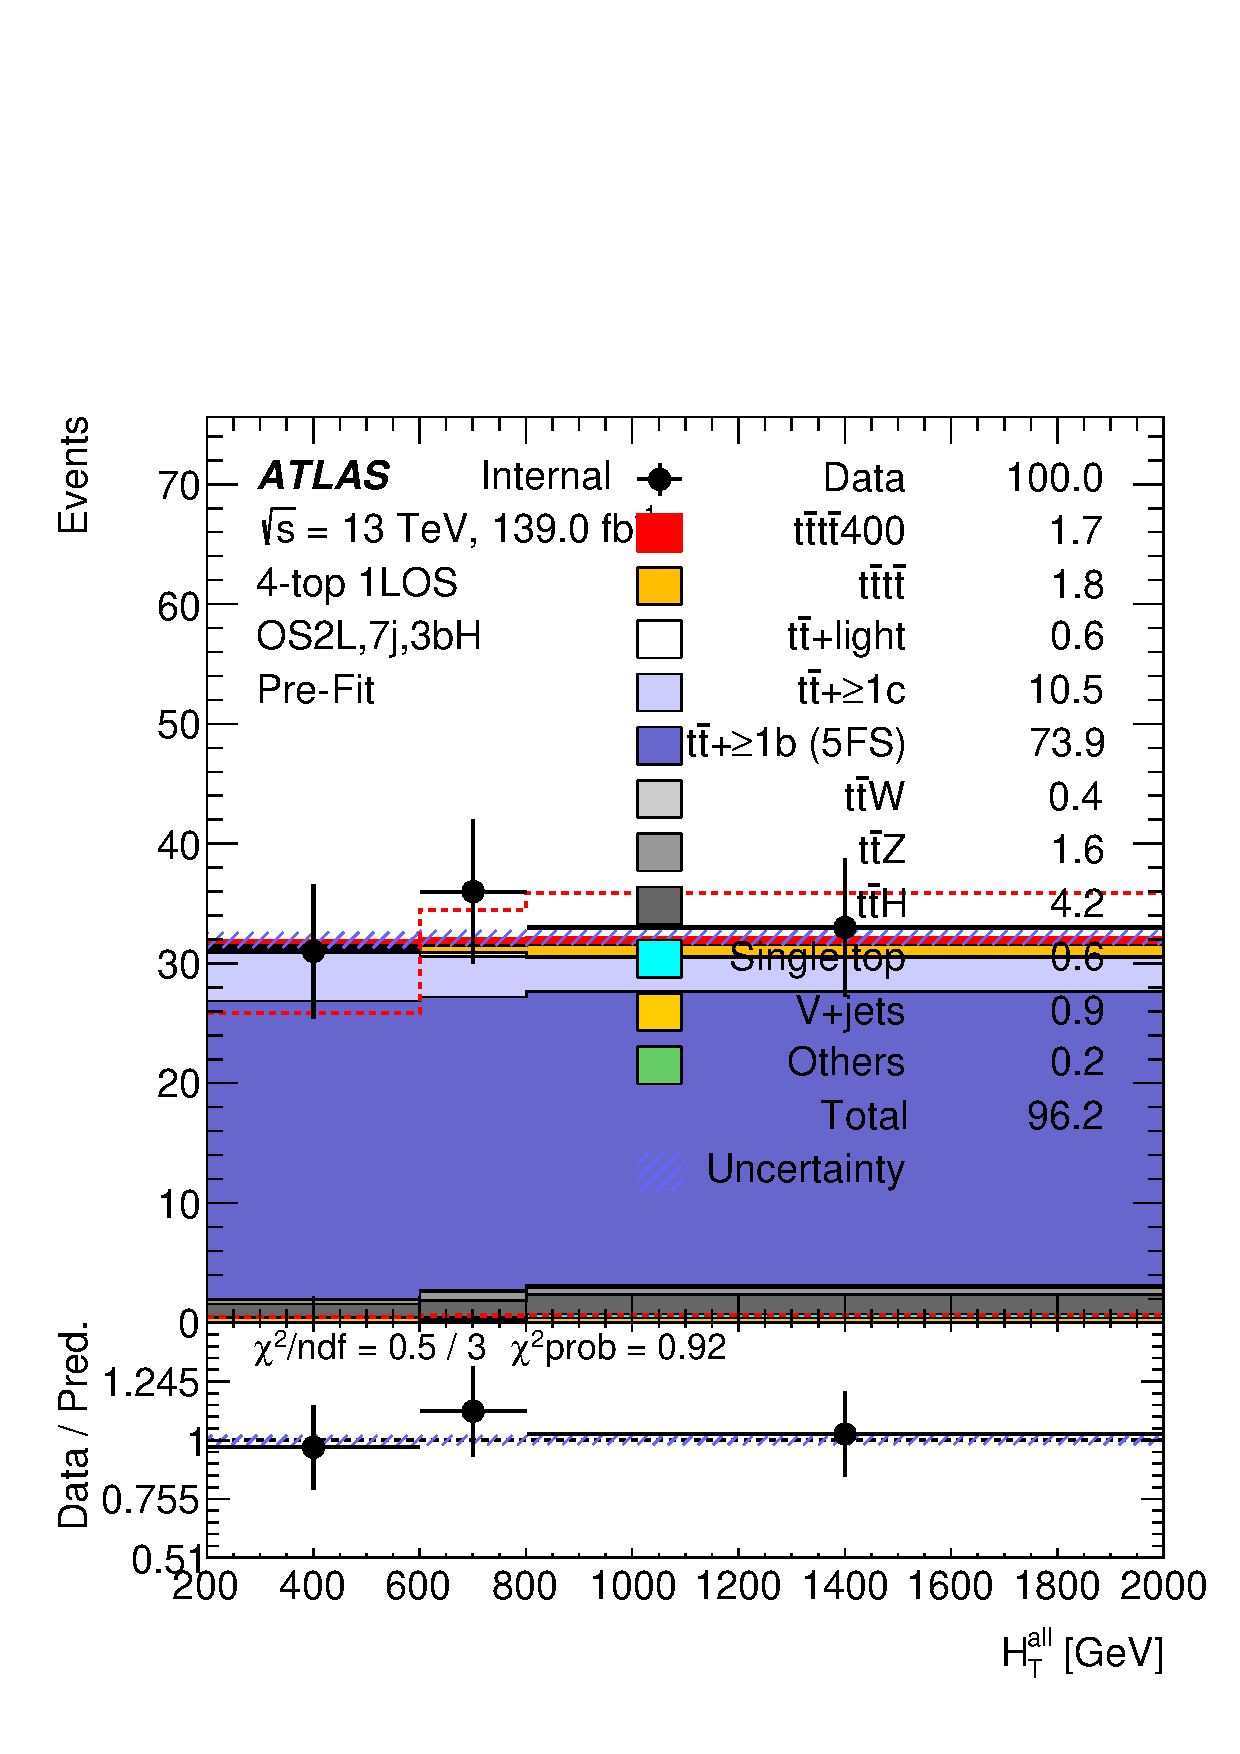
\includegraphics[width=0.23 \textwidth]{figures/fits/4FSvs5FS/GNN/400/Data_to_MC_5FS/os2l_7j3bH.pdf} \\                                                                   
                                                                                                                                                                            
      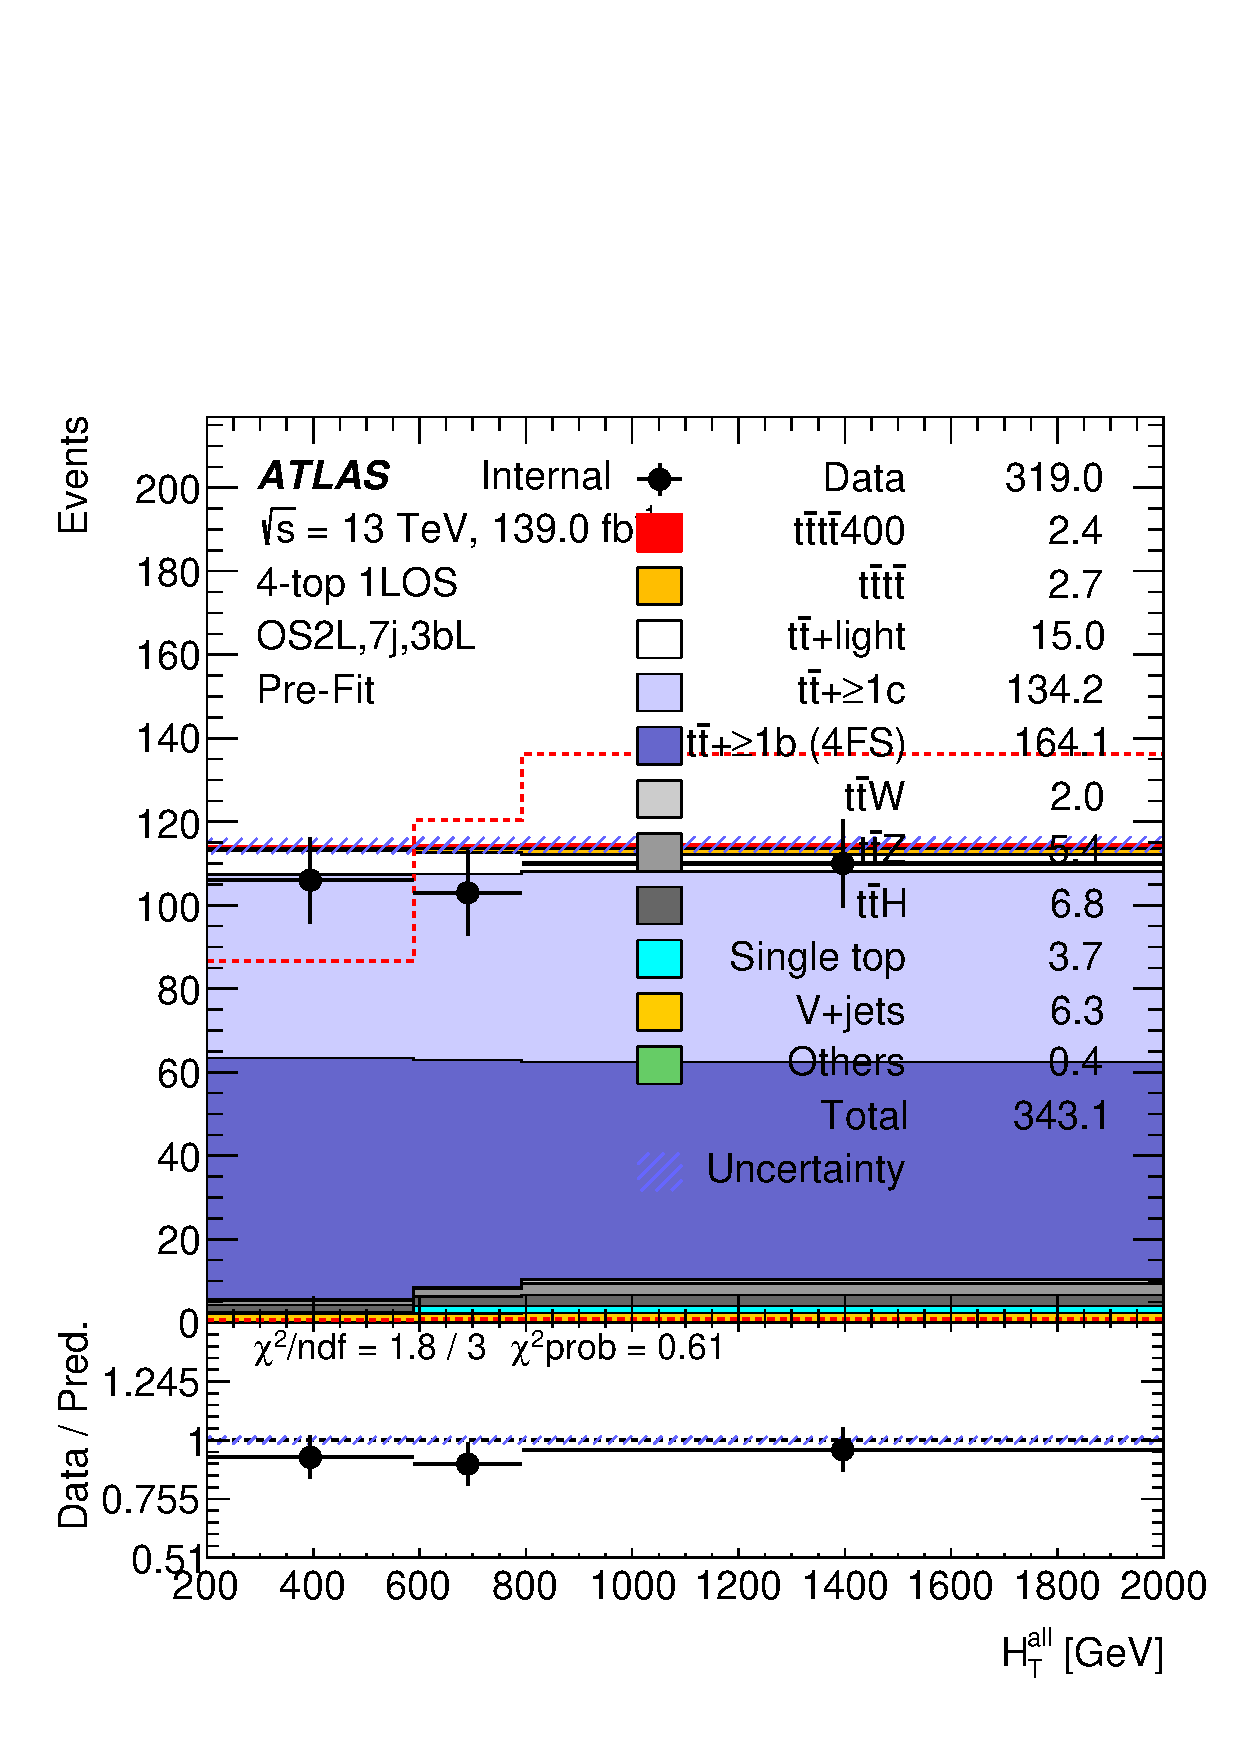
\includegraphics[width=0.23 \textwidth]{figures/fits/4FSvs5FS/GNN/400/Data_to_MC_4FS/os2l_7j3bL.pdf} &                                                                      
      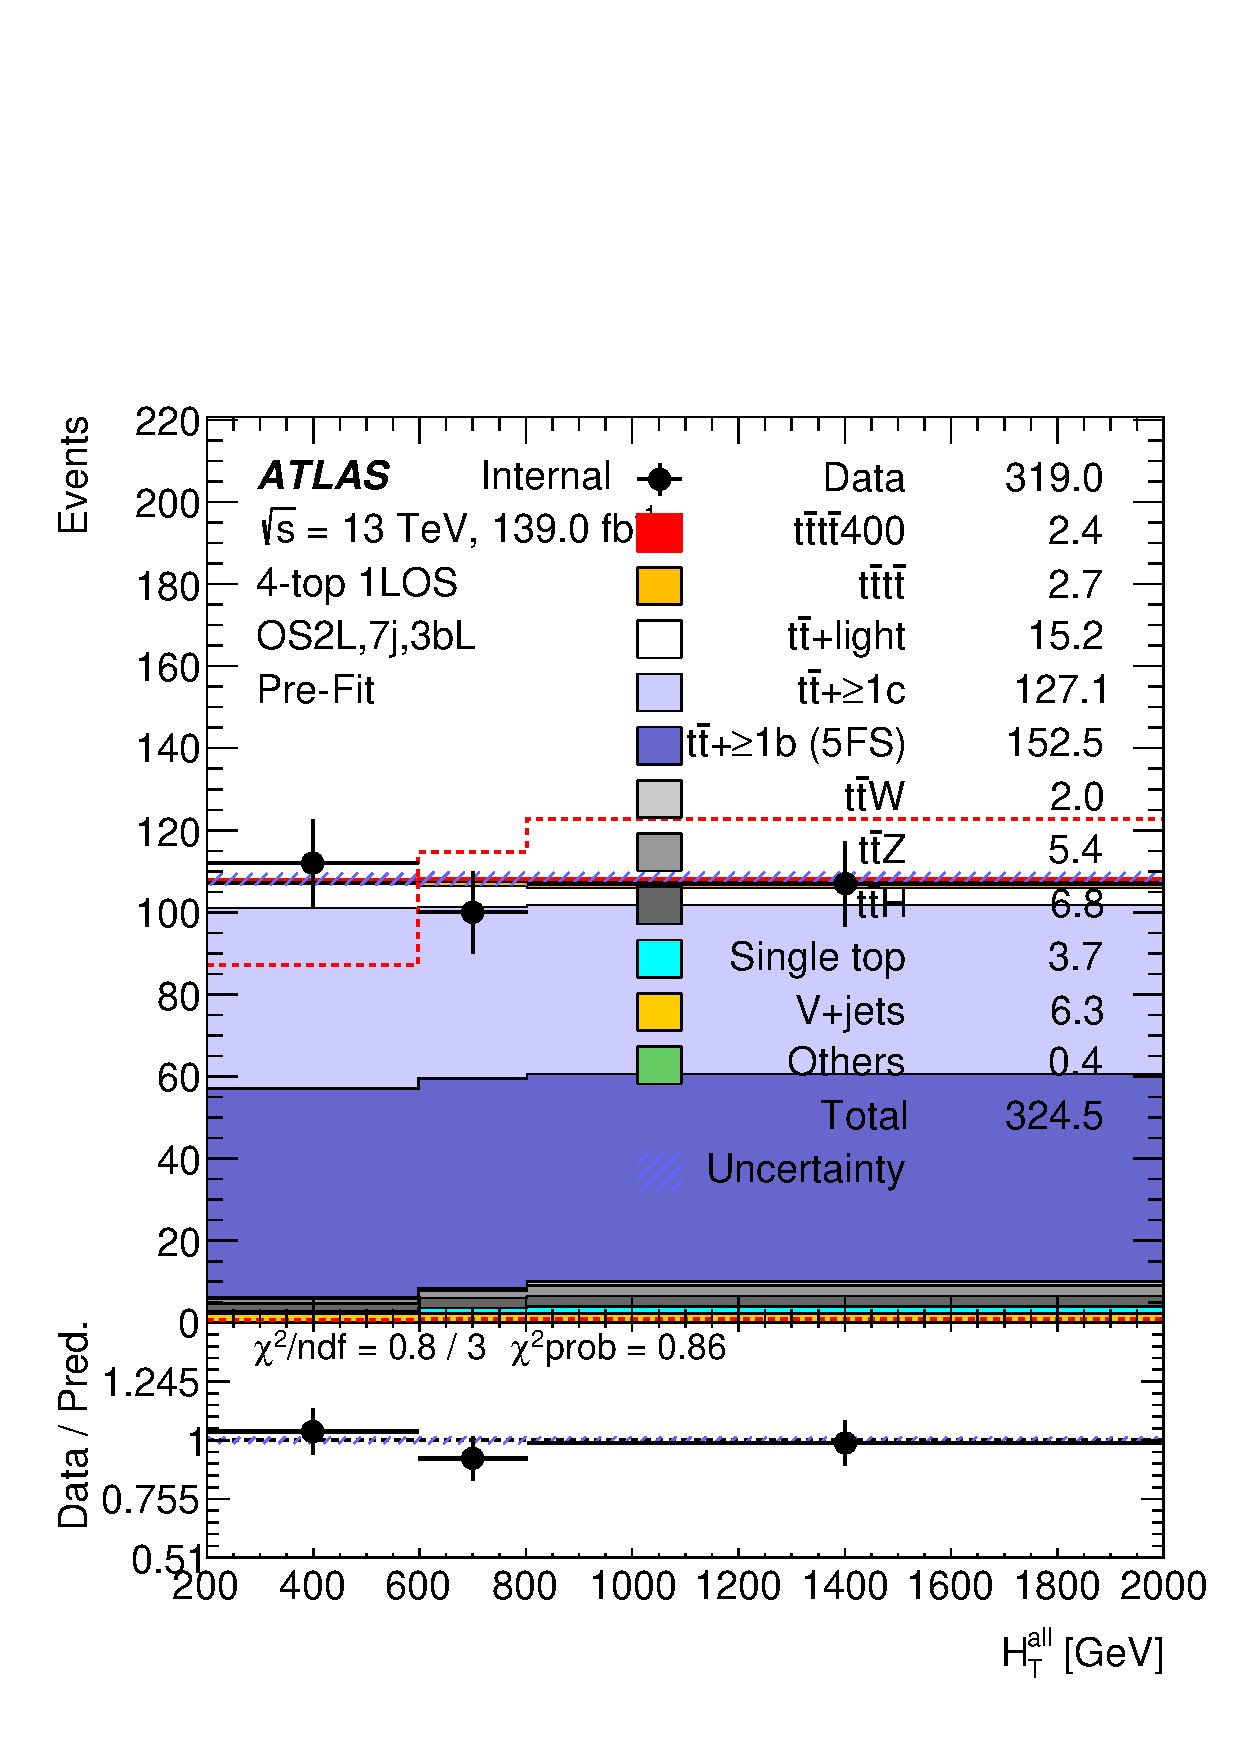
\includegraphics[width=0.23 \textwidth]{figures/fits/4FSvs5FS/GNN/400/Data_to_MC_5FS/os2l_7j3bL.pdf} &                                                                      
      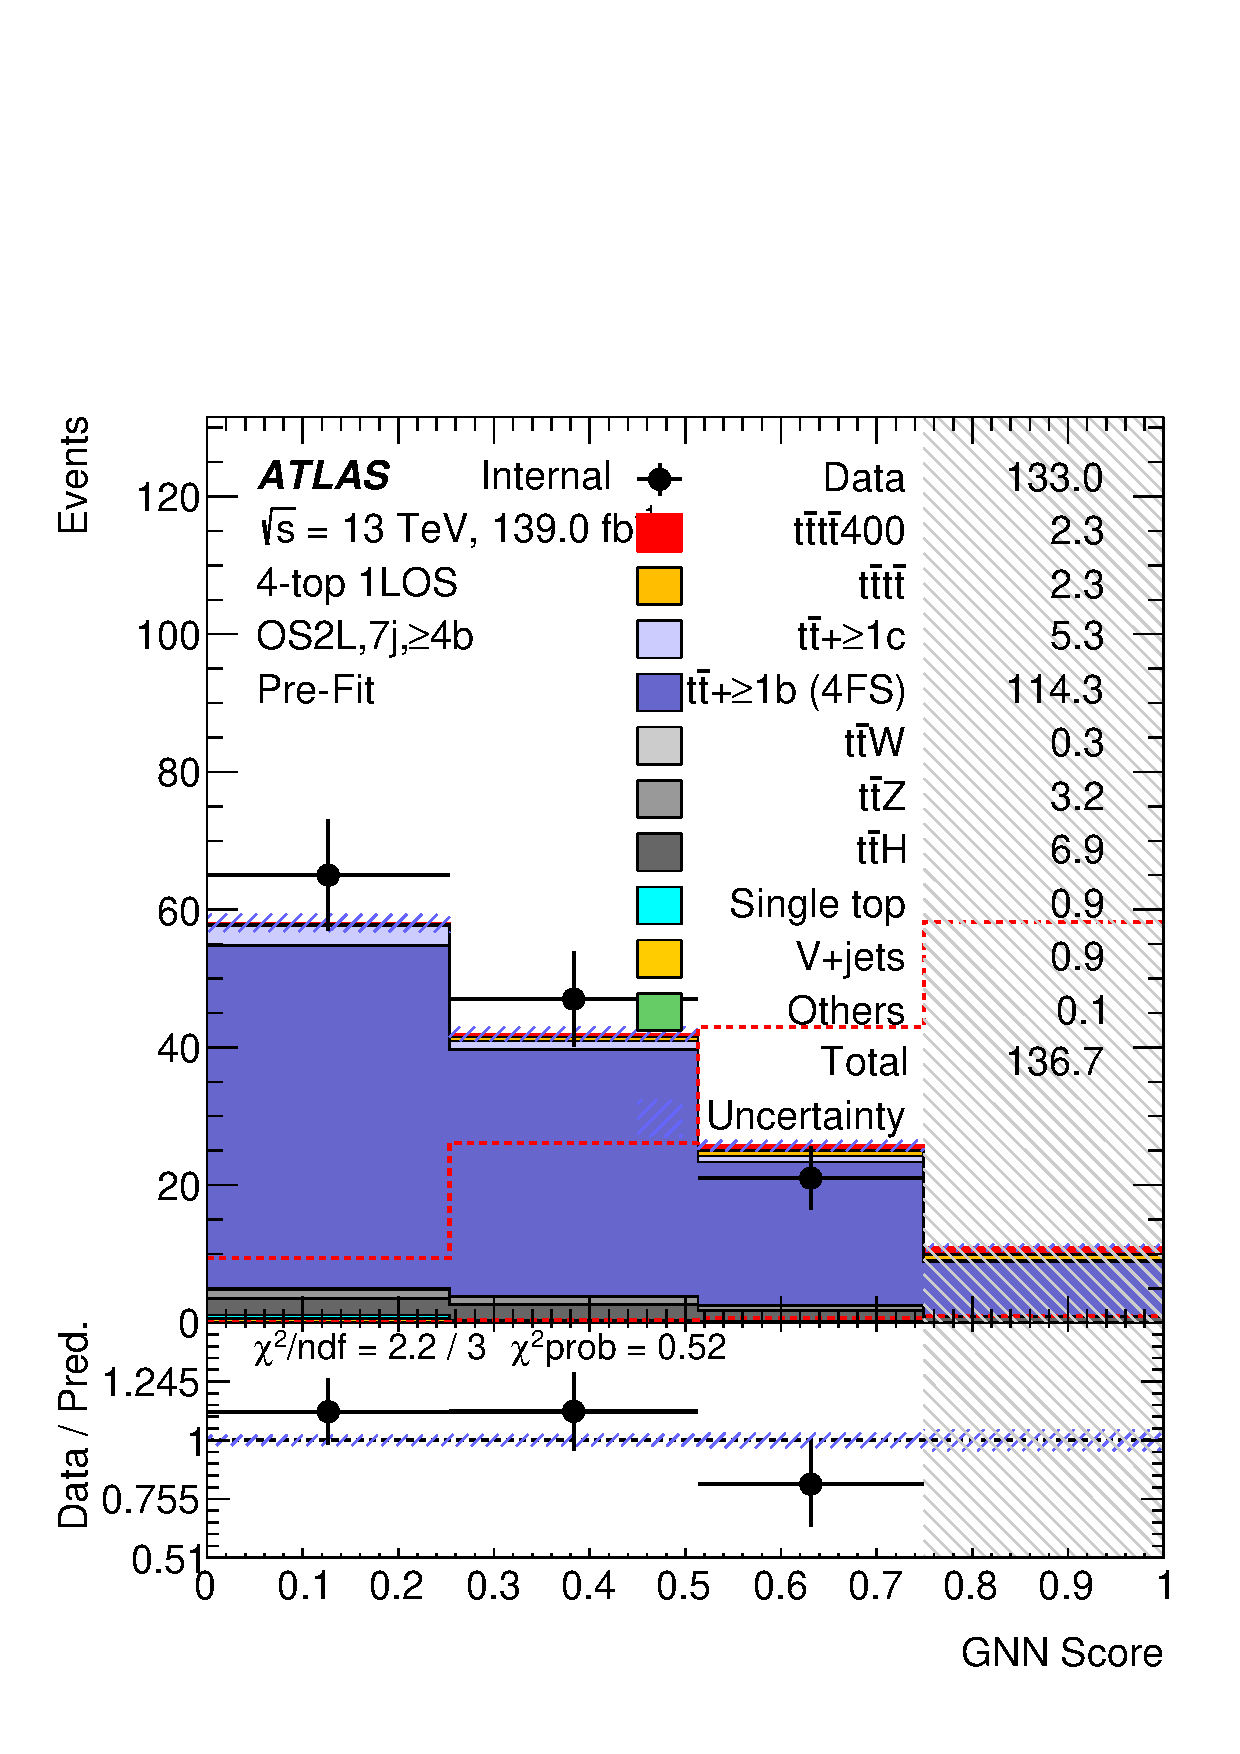
\includegraphics[width=0.23 \textwidth]{figures/fits/4FSvs5FS/GNN/400/Data_to_MC_4FS/os2l_7jge4b.pdf} &                                                                     
      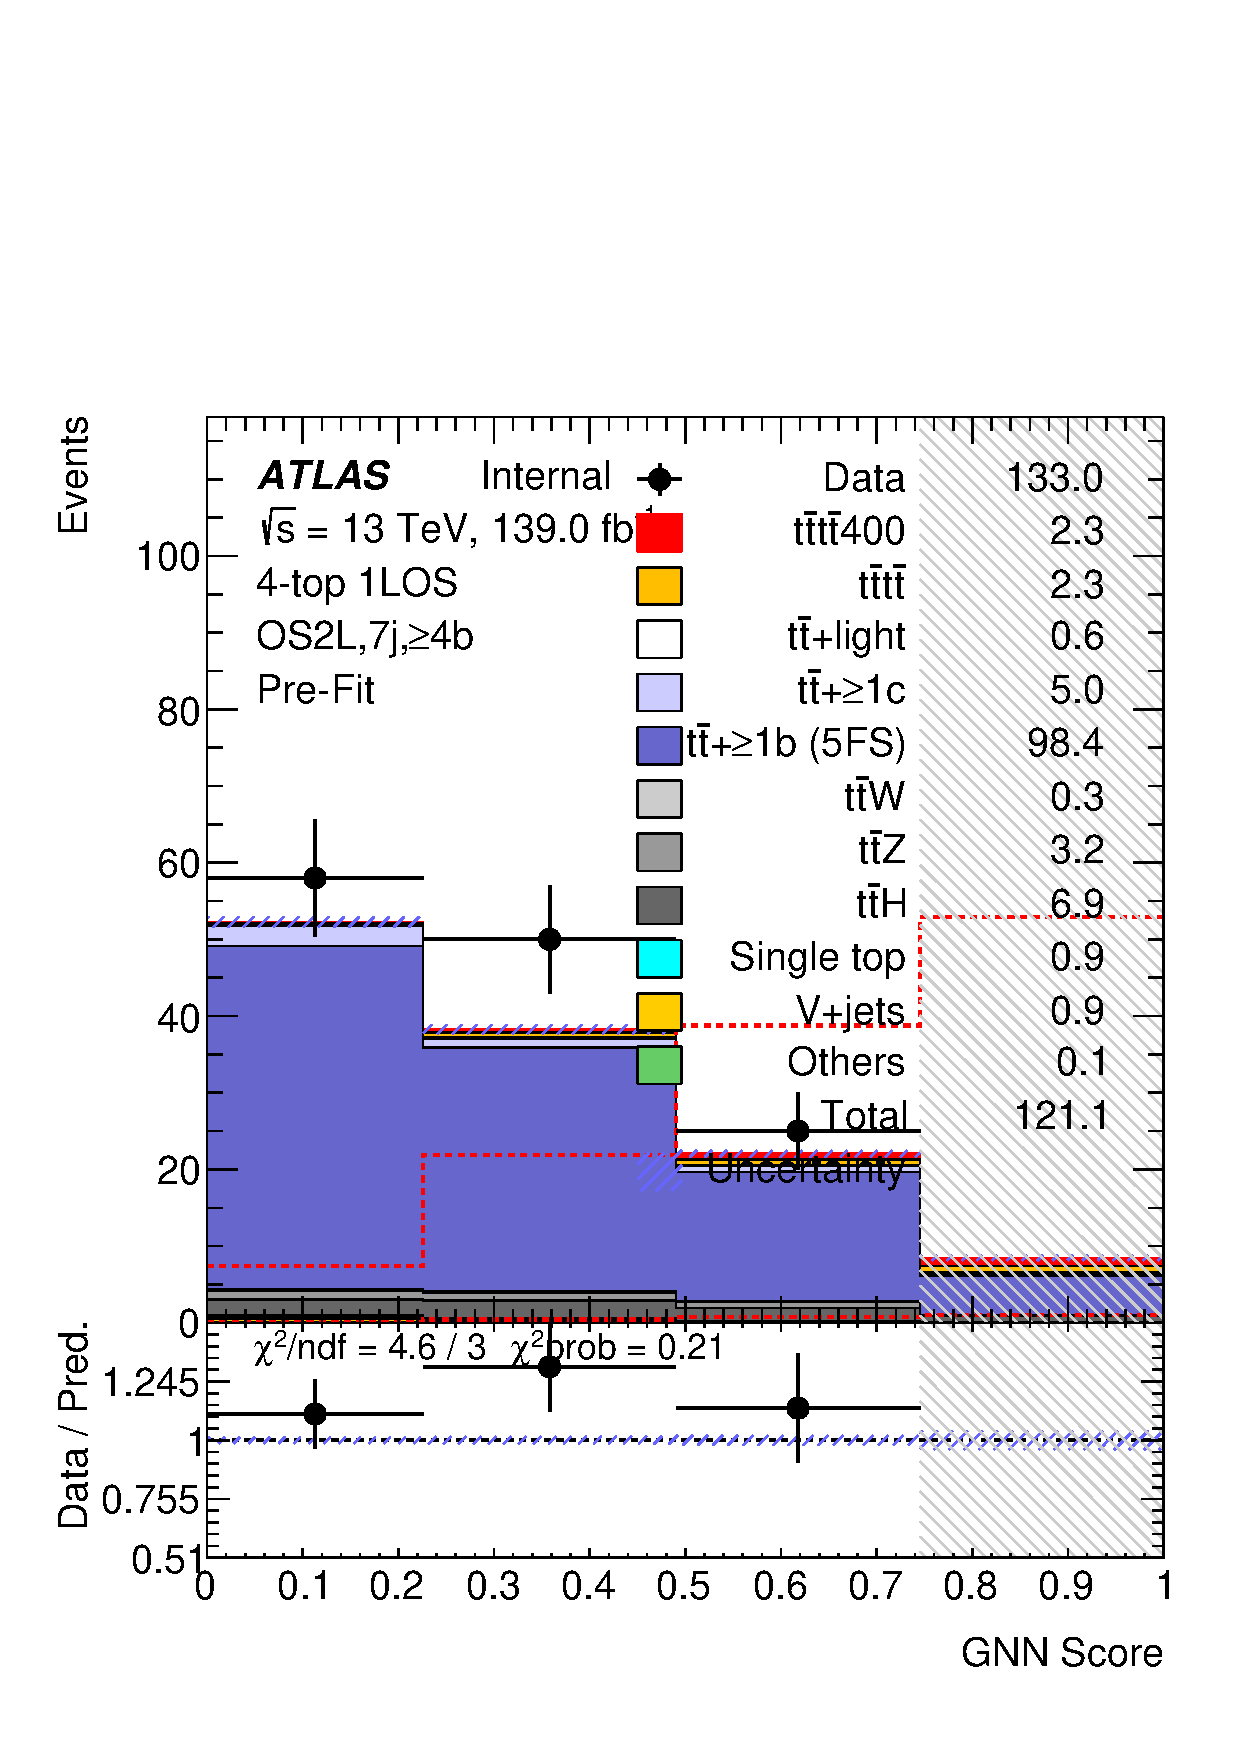
\includegraphics[width=0.23 \textwidth]{figures/fits/4FSvs5FS/GNN/400/Data_to_MC_5FS/os2l_7jge4b.pdf} \\                                                                     

      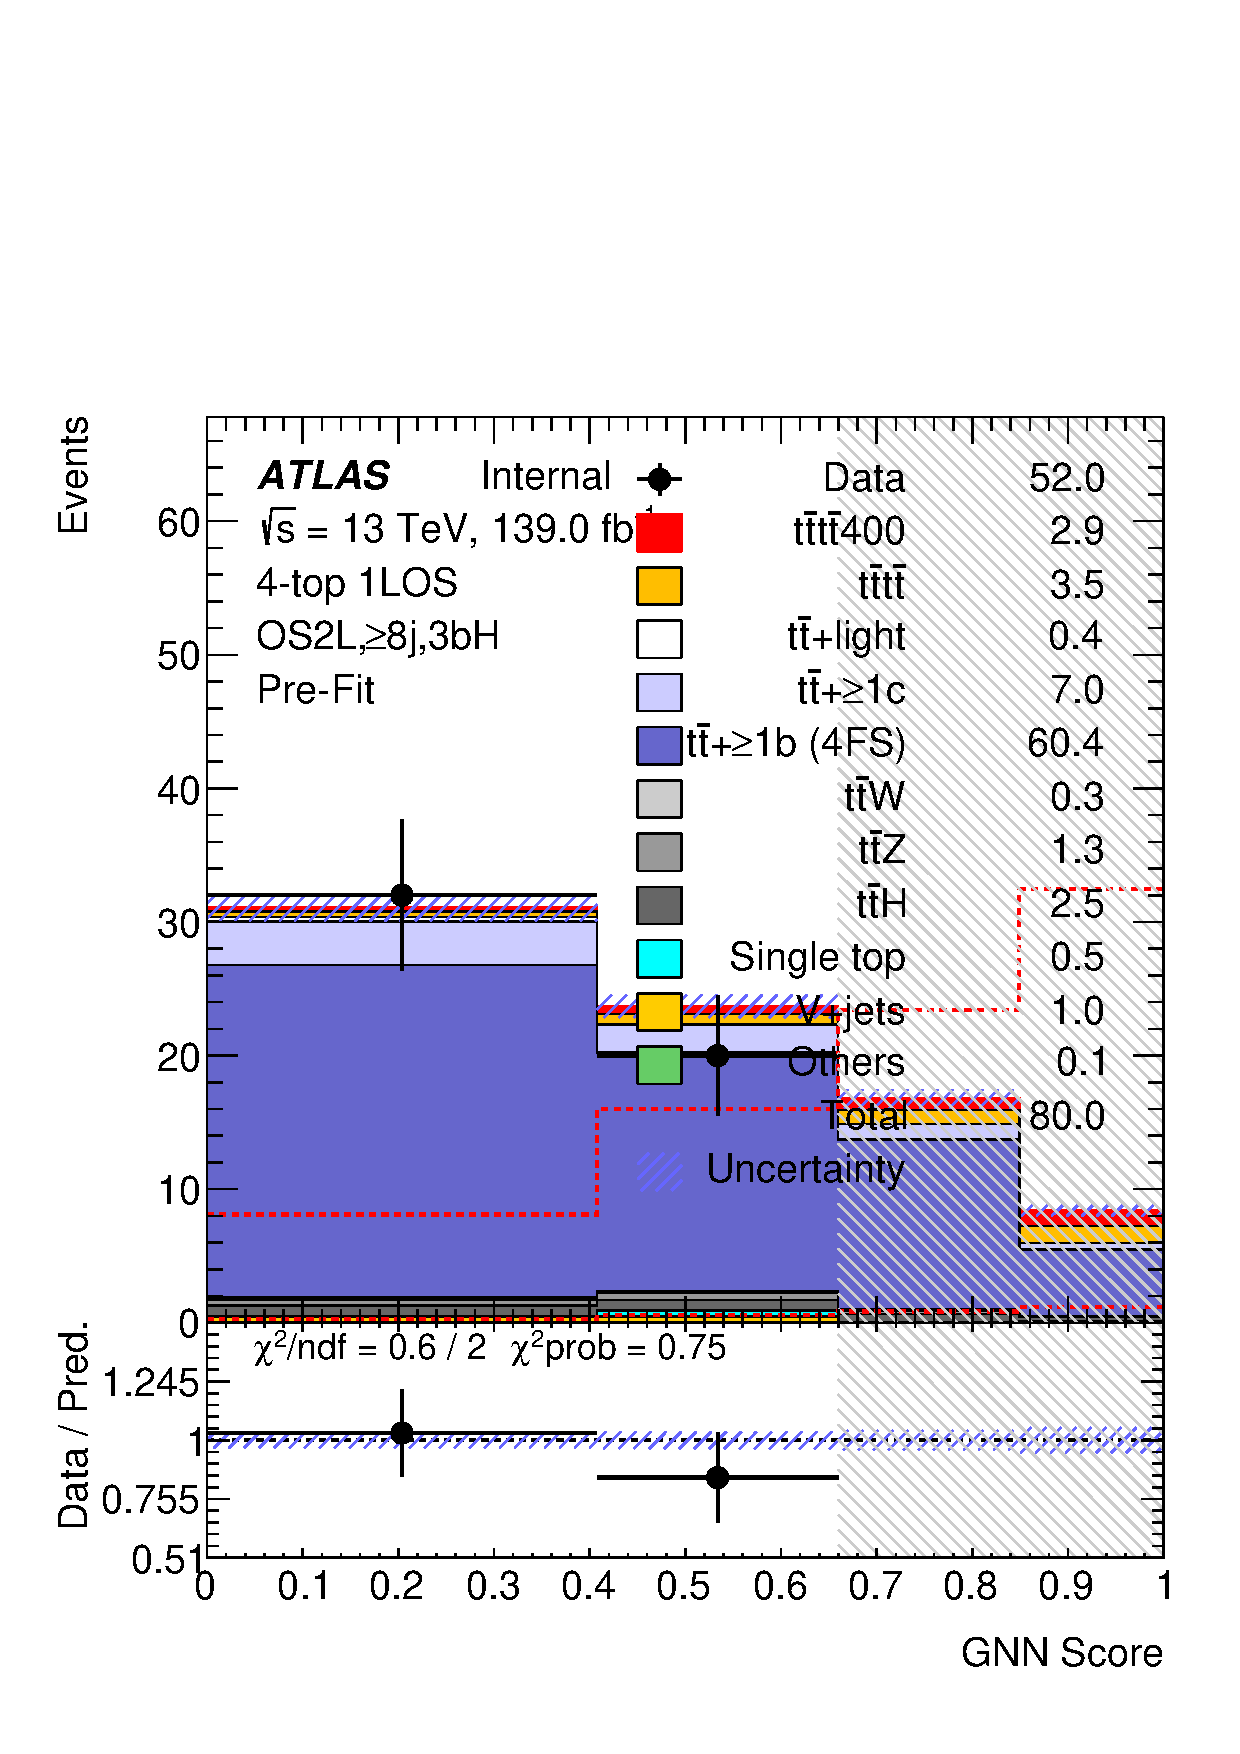
\includegraphics[width=0.23 \textwidth]{figures/fits/4FSvs5FS/GNN/400/Data_to_MC_4FS/os2l_ge8j3bH.pdf} &                                                                     
      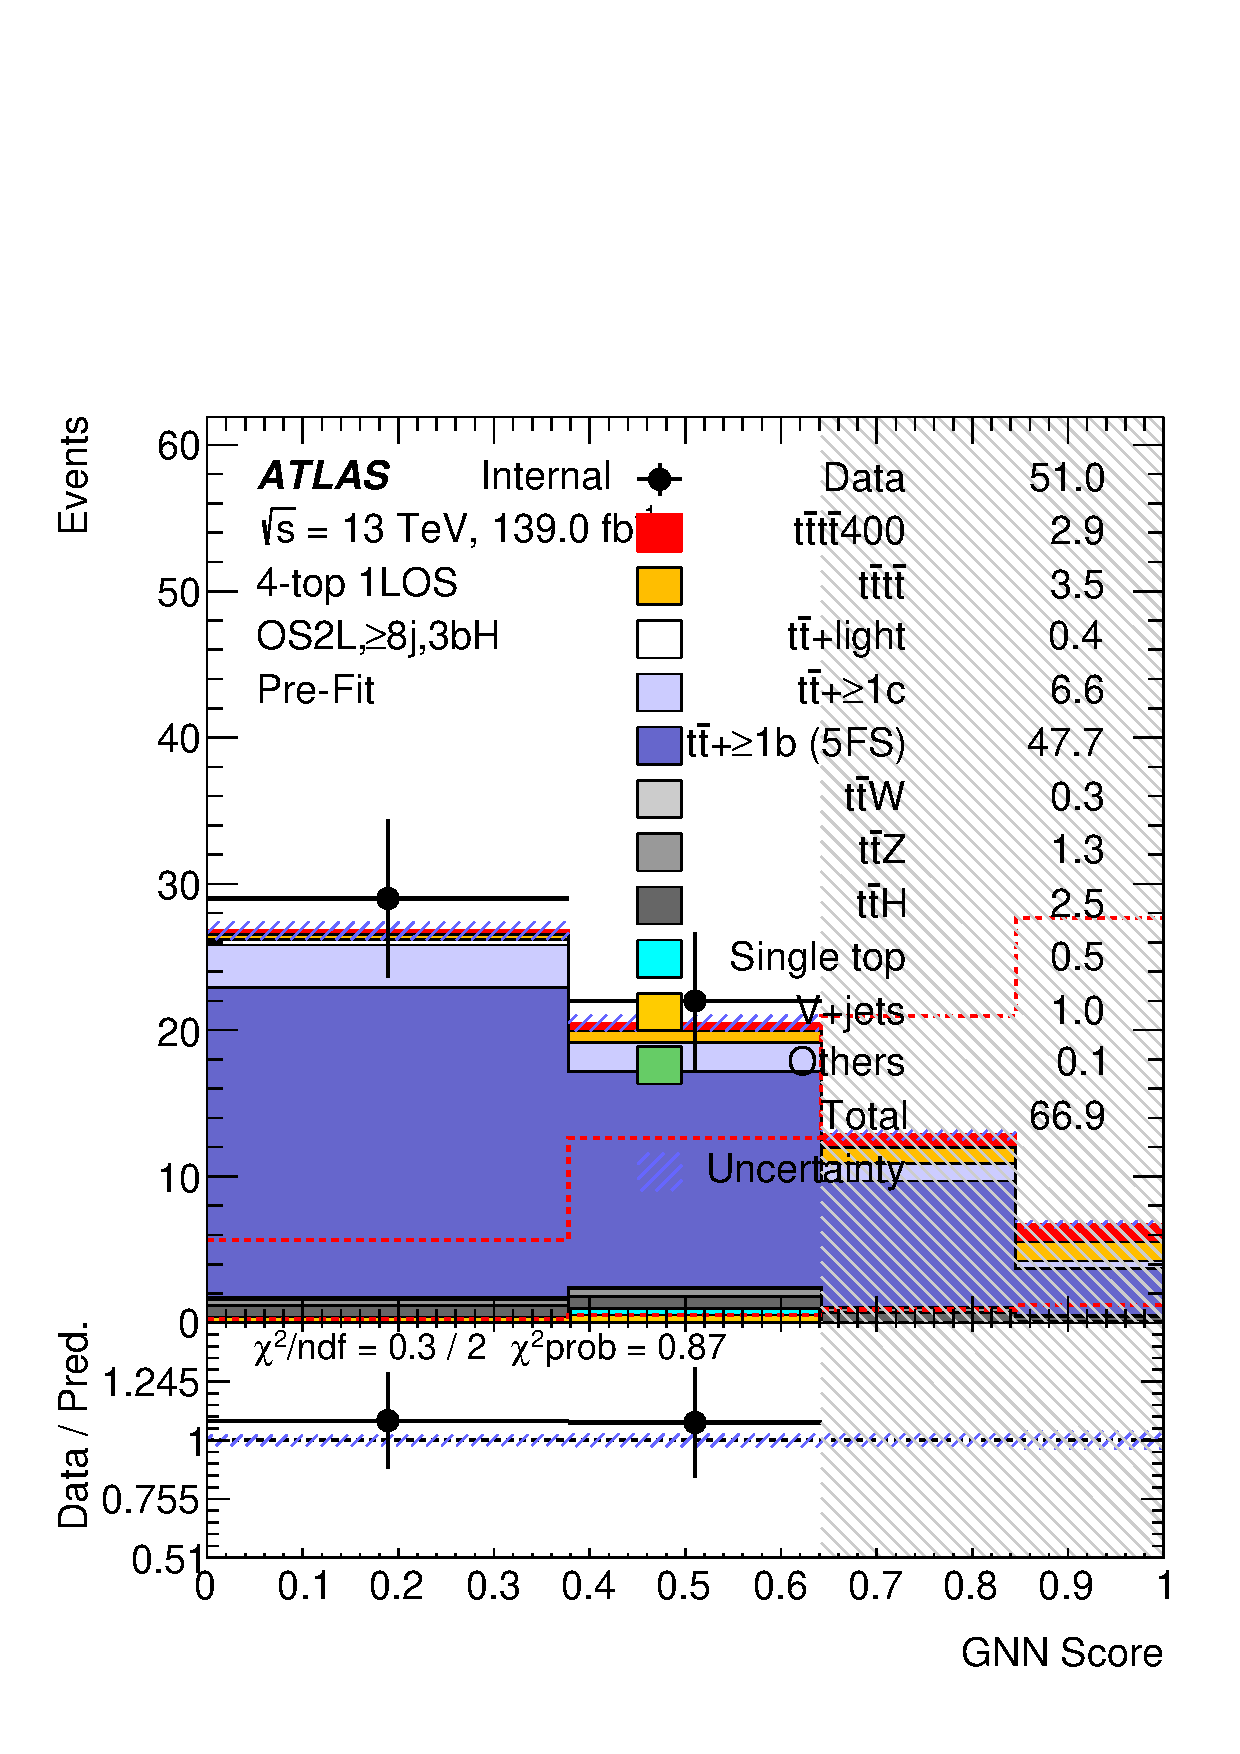
\includegraphics[width=0.23 \textwidth]{figures/fits/4FSvs5FS/GNN/400/Data_to_MC_5FS/os2l_ge8j3bH.pdf} &                                                                     
      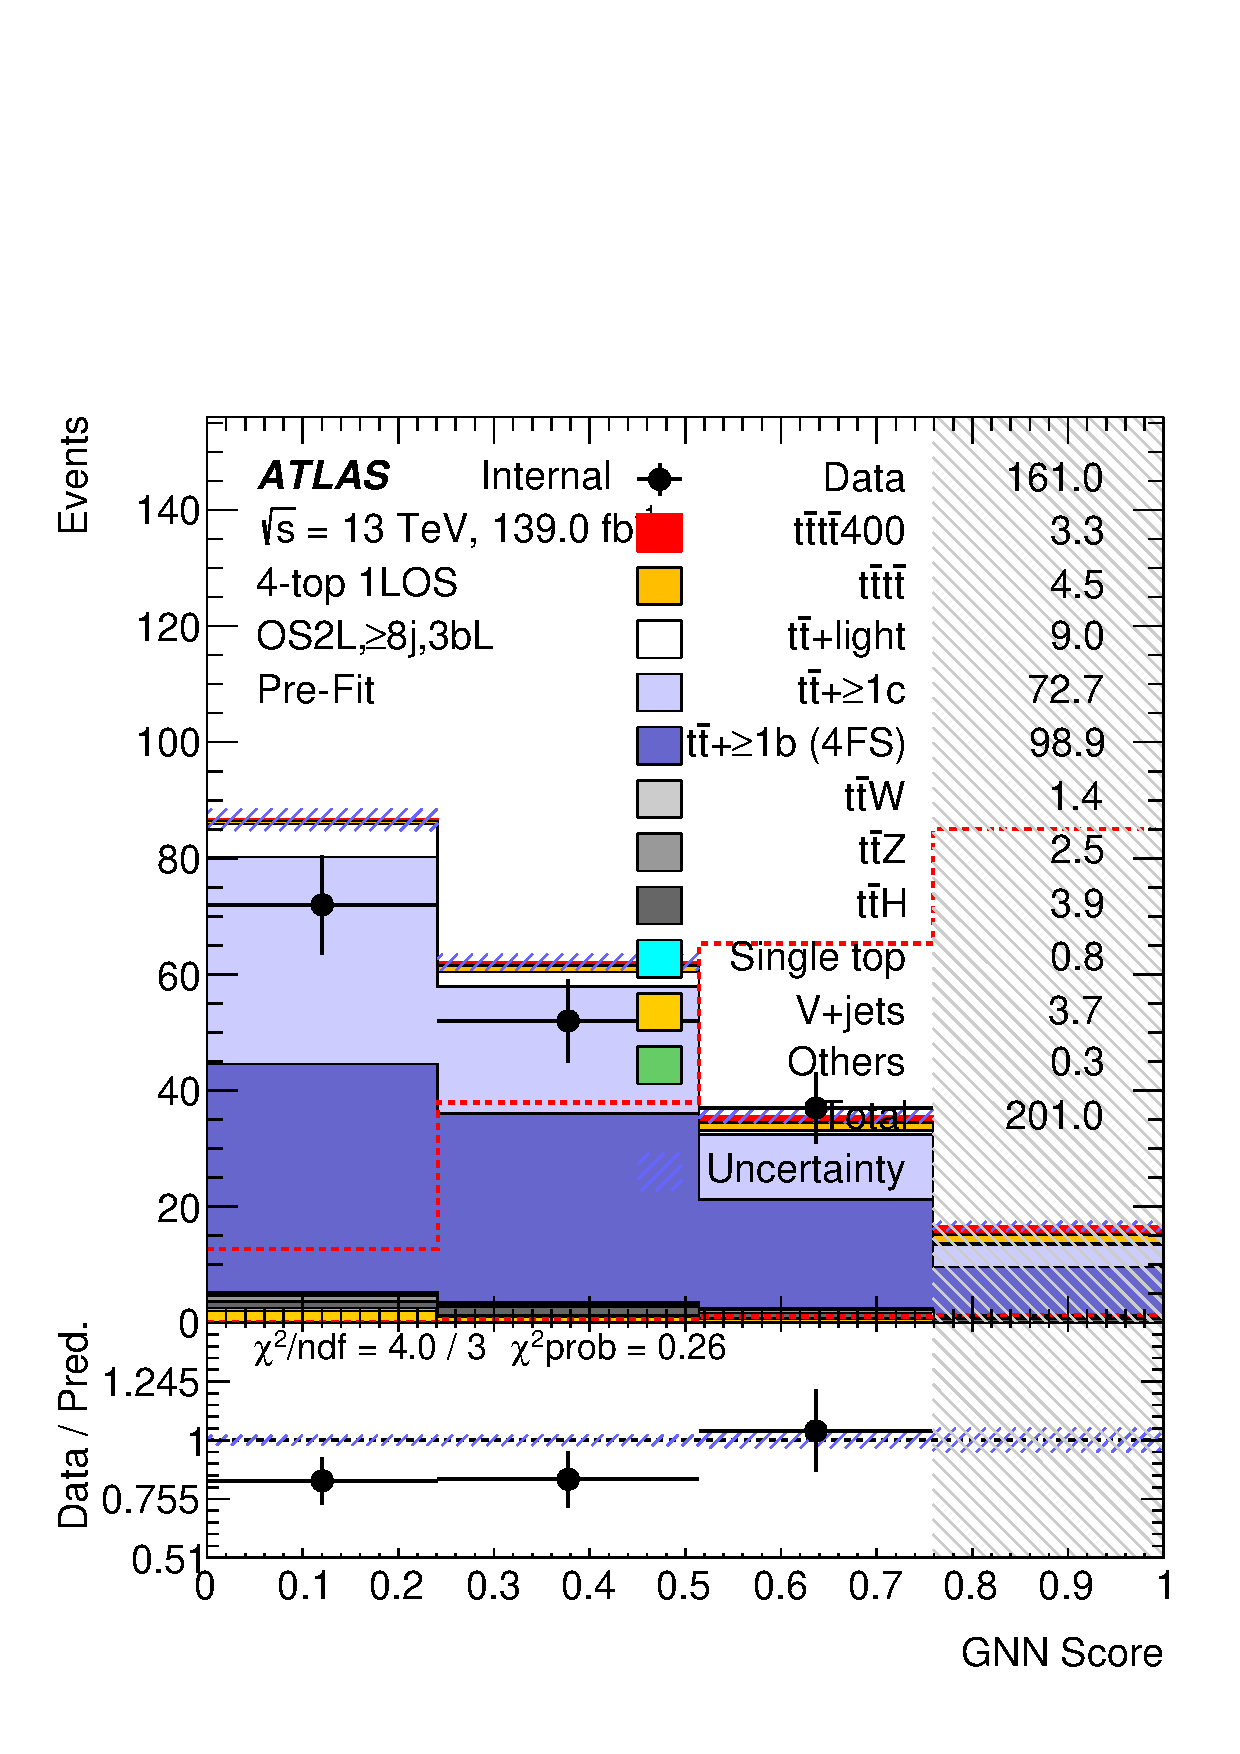
\includegraphics[width=0.23 \textwidth]{figures/fits/4FSvs5FS/GNN/400/Data_to_MC_4FS/os2l_ge8j3bL.pdf} &                                                                     
      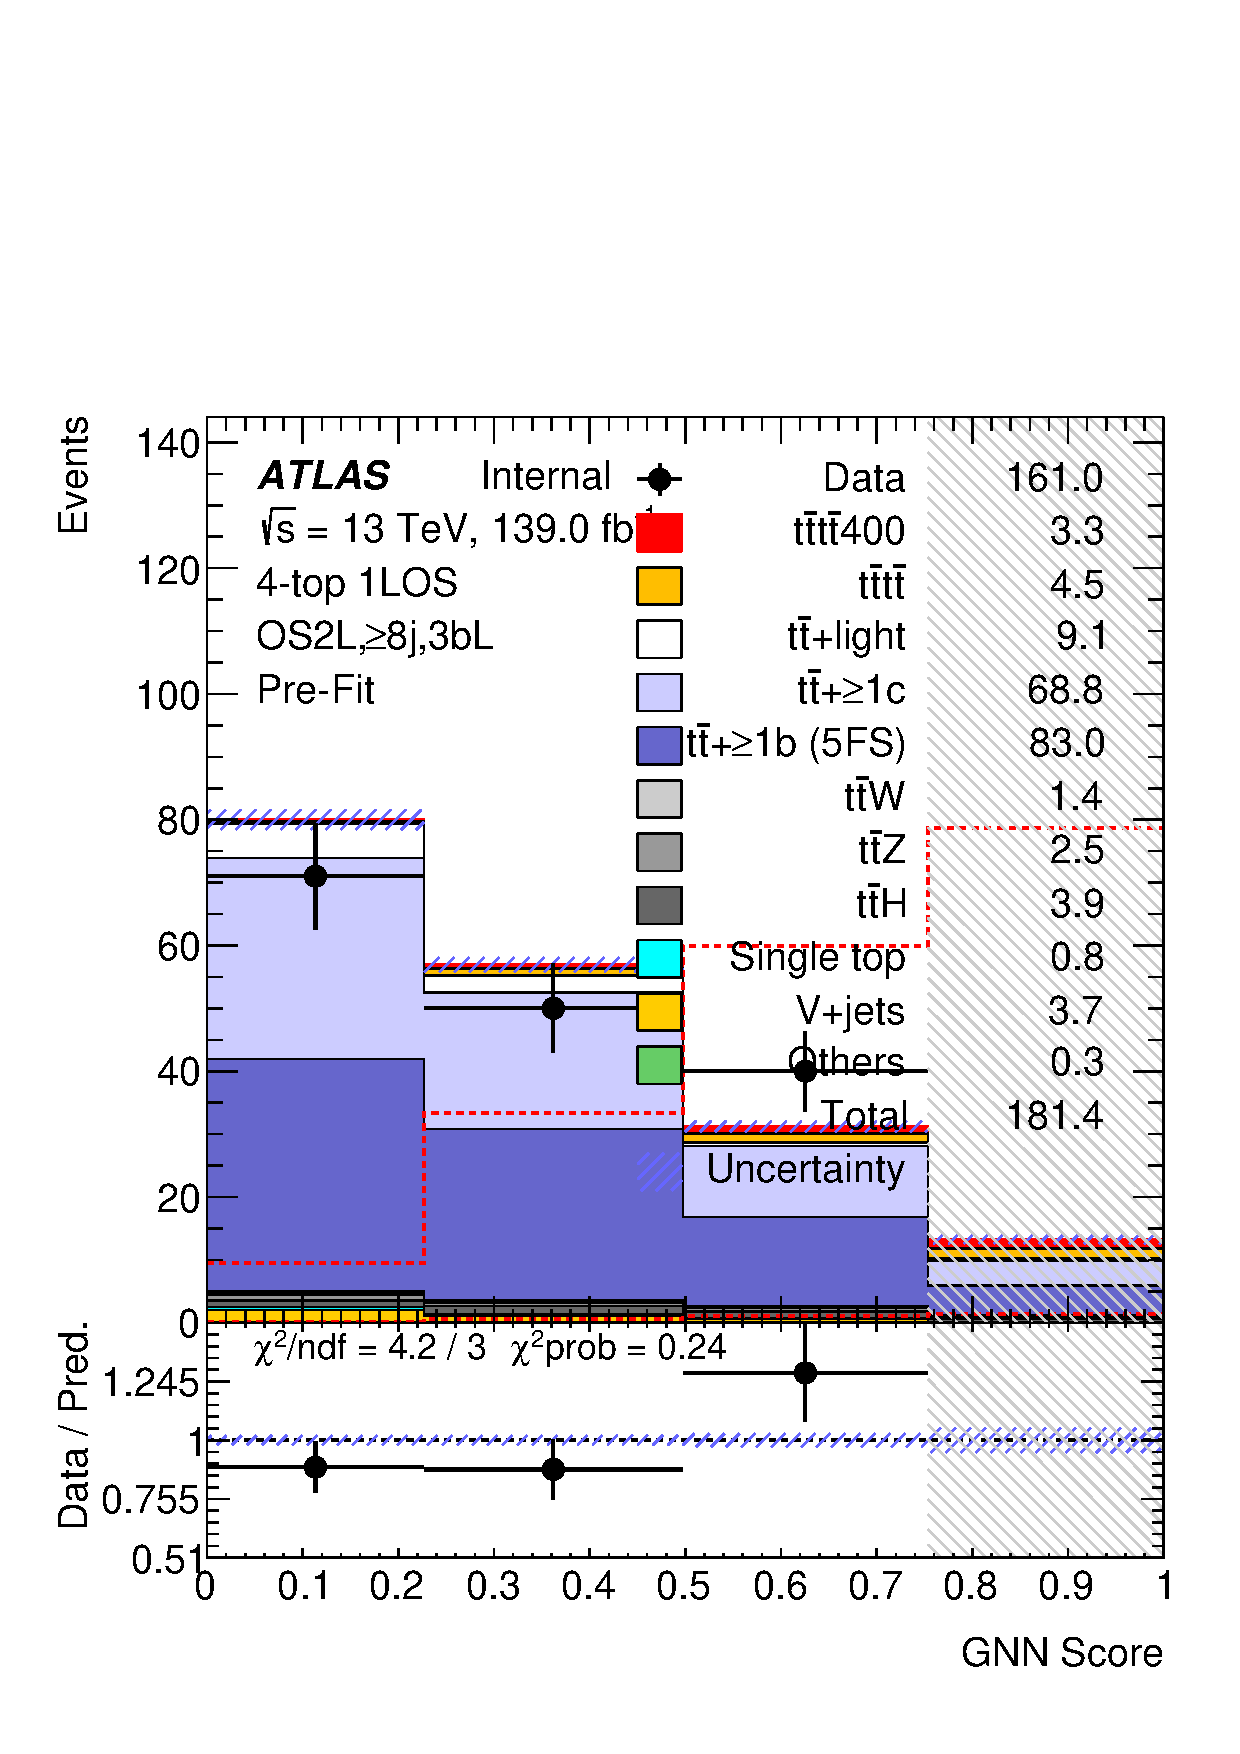
\includegraphics[width=0.23 \textwidth]{figures/fits/4FSvs5FS/GNN/400/Data_to_MC_5FS/os2l_ge8j3bL.pdf} \\ 
      
      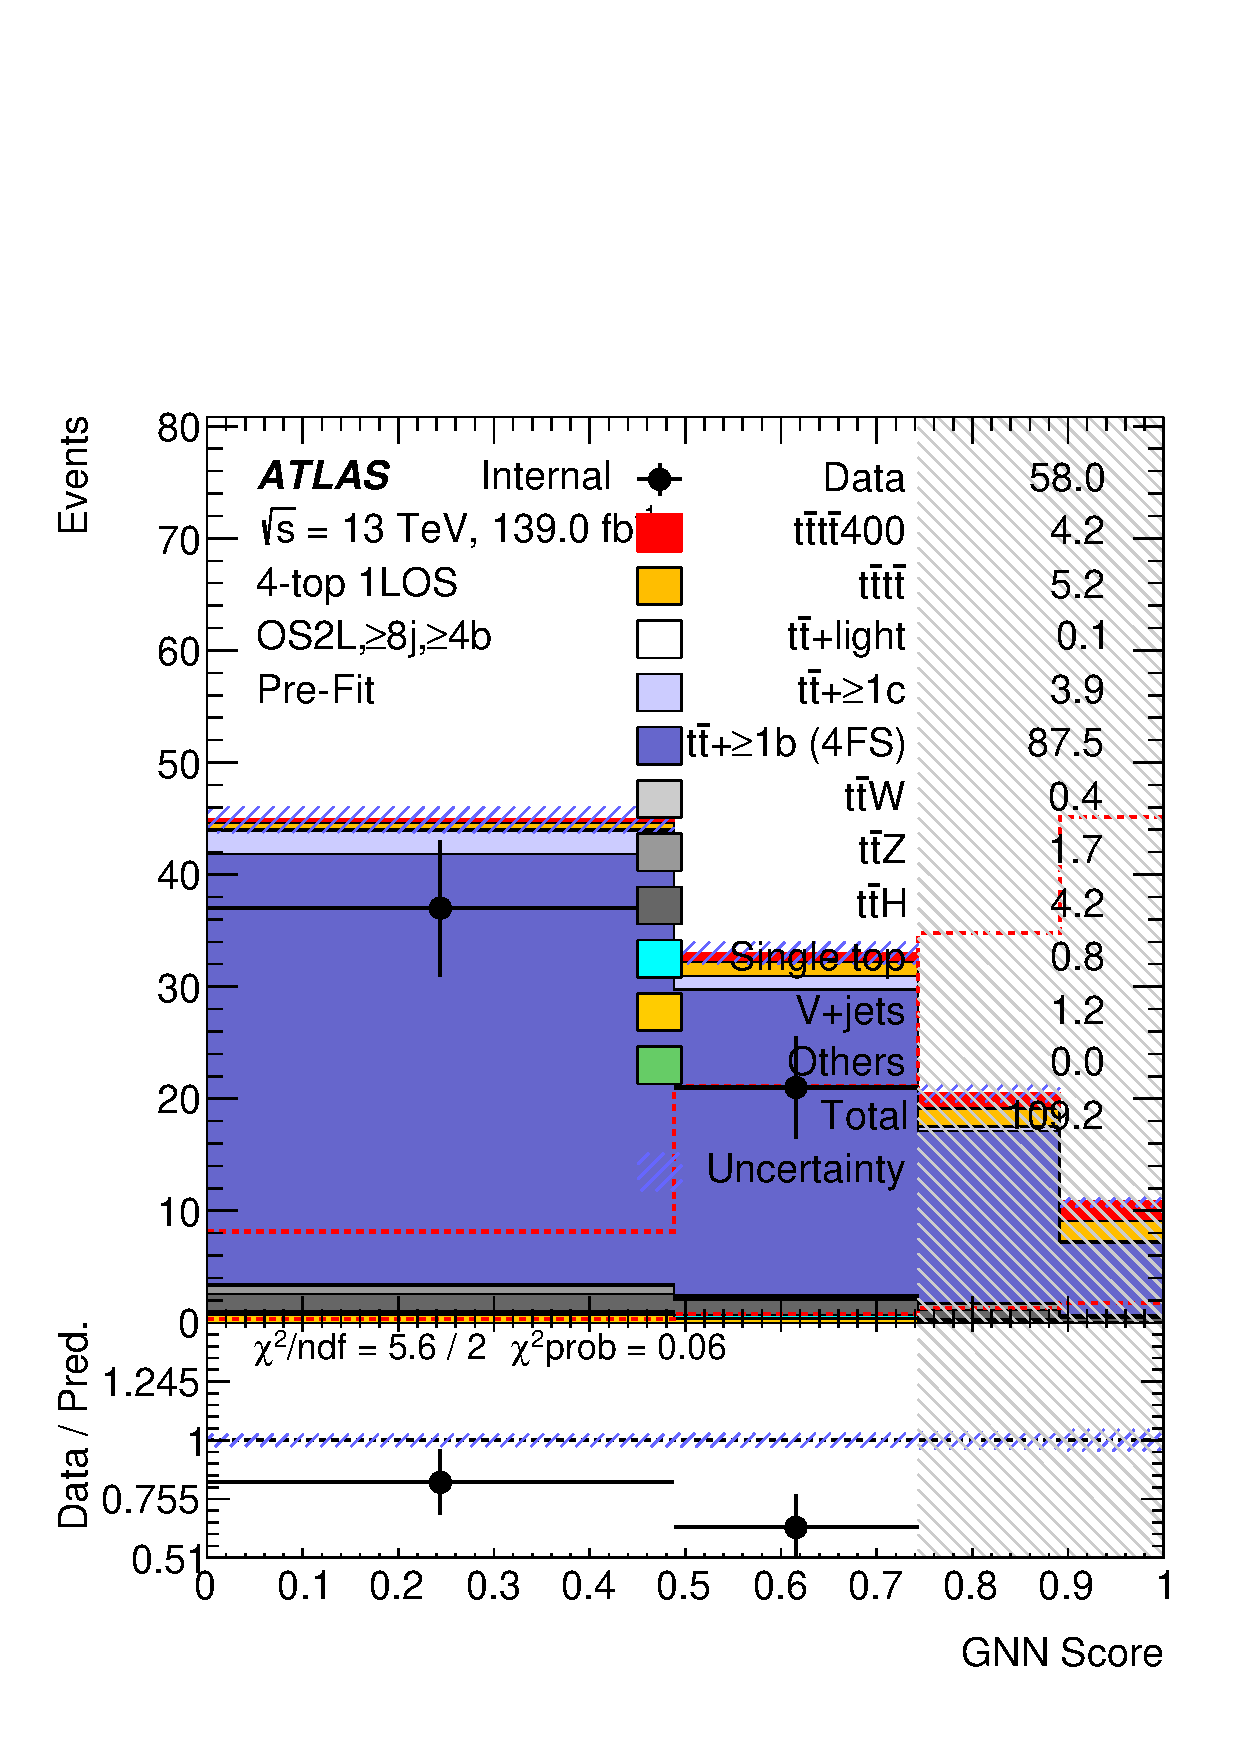
\includegraphics[width=0.23 \textwidth]{figures/fits/4FSvs5FS/GNN/400/Data_to_MC_4FS/os2l_ge8jge4b.pdf} &                                                                    
      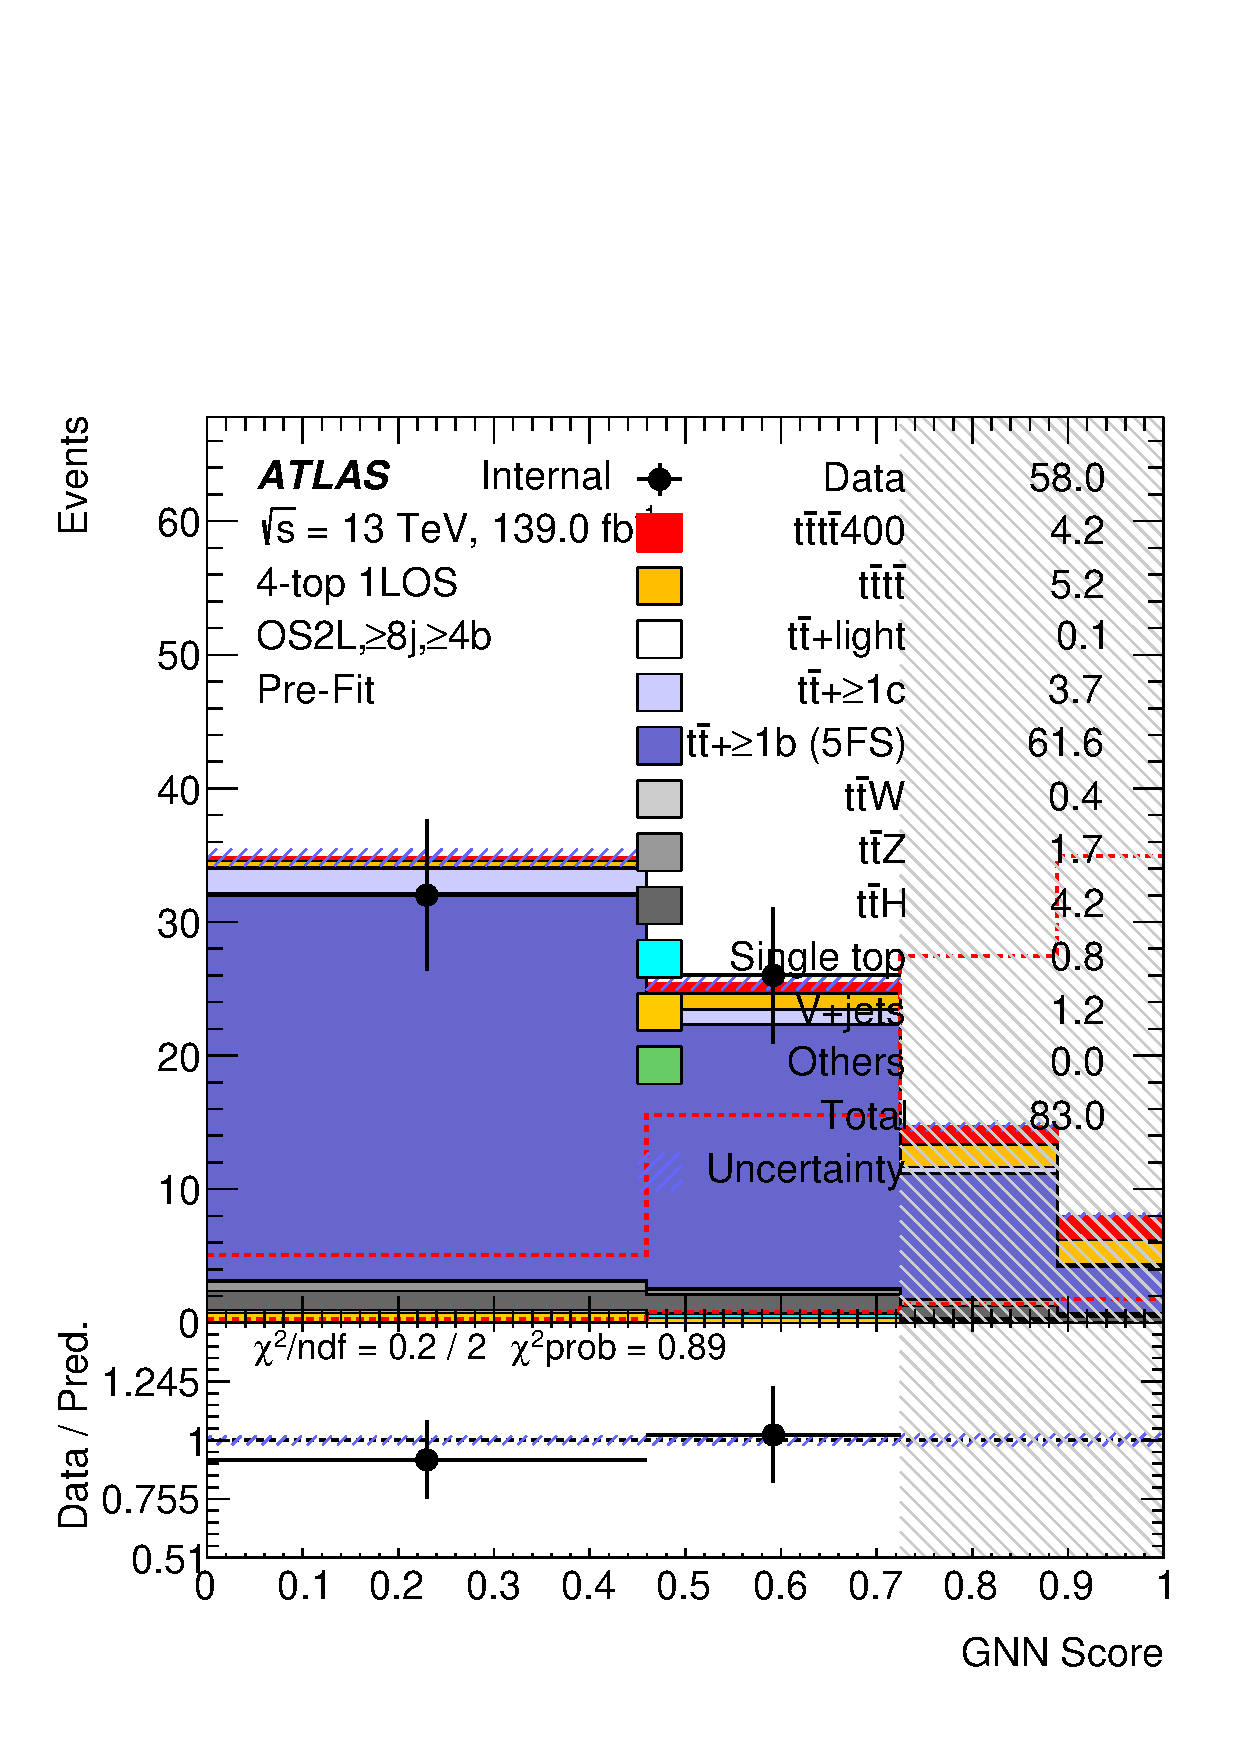
\includegraphics[width=0.23 \textwidth]{figures/fits/4FSvs5FS/GNN/400/Data_to_MC_5FS/os2l_ge8jge4b.pdf} \\
    \end{tabular}                                                                                                                                                                
    \caption{\label{4FSvs5FS_dataMC_2LOS}Pre-fit distributions in 5FS compared with 4FS for 2LOS channel associated with different signal and background samples, compared with data yields.}  
  \end{center}                                                                                                                                                                     
\end{figure}




\begin{figure}[htbp!]                                                                                                                                                              
\begin{center} \setlength{\tabcolsep}{2.5pt}\footnotesize                                                                                                                          
\begin{tabular}{cccc}    

      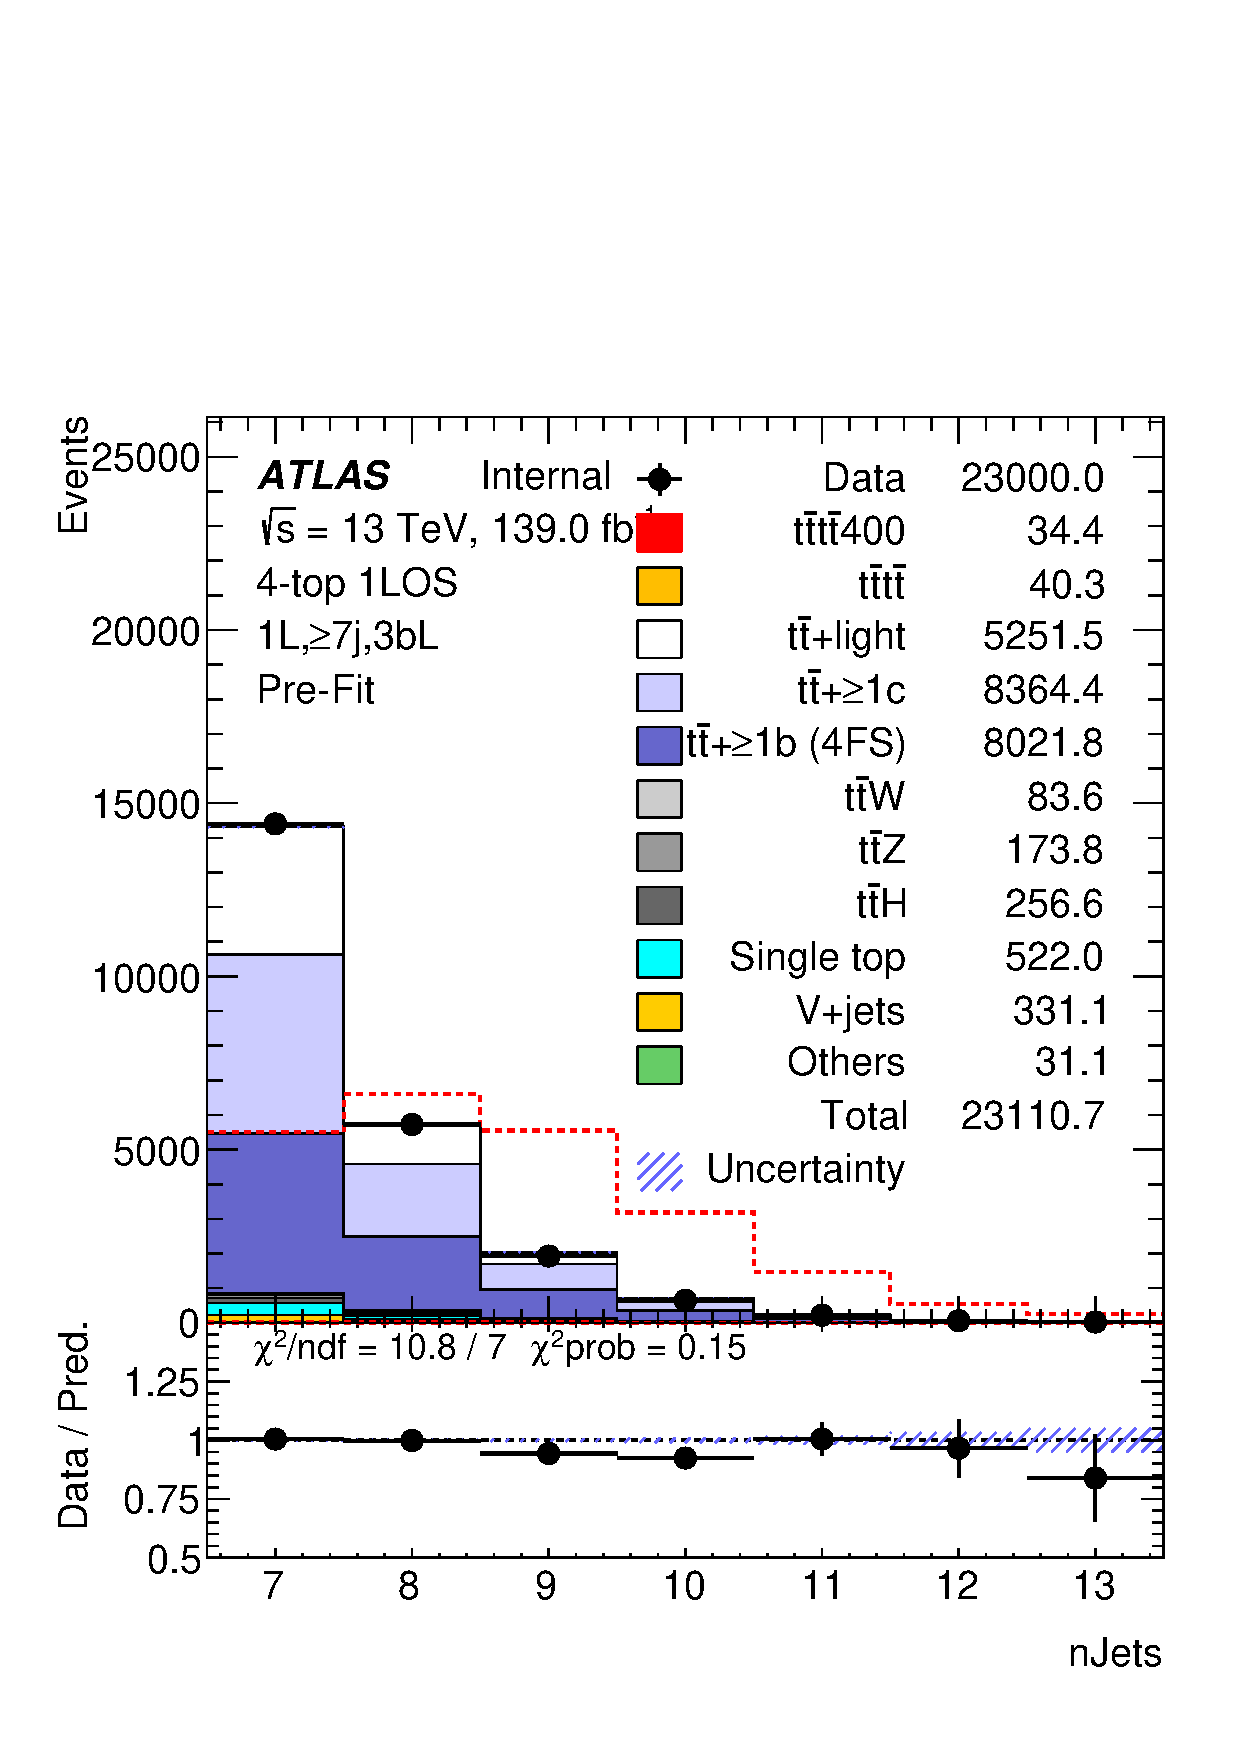
\includegraphics[width=0.25 \textwidth]{figures/fits/4FSvs5FS/GNN/400/Data_to_MC_4FS/val_ljets_ge7j3bL.pdf} &                                                  
      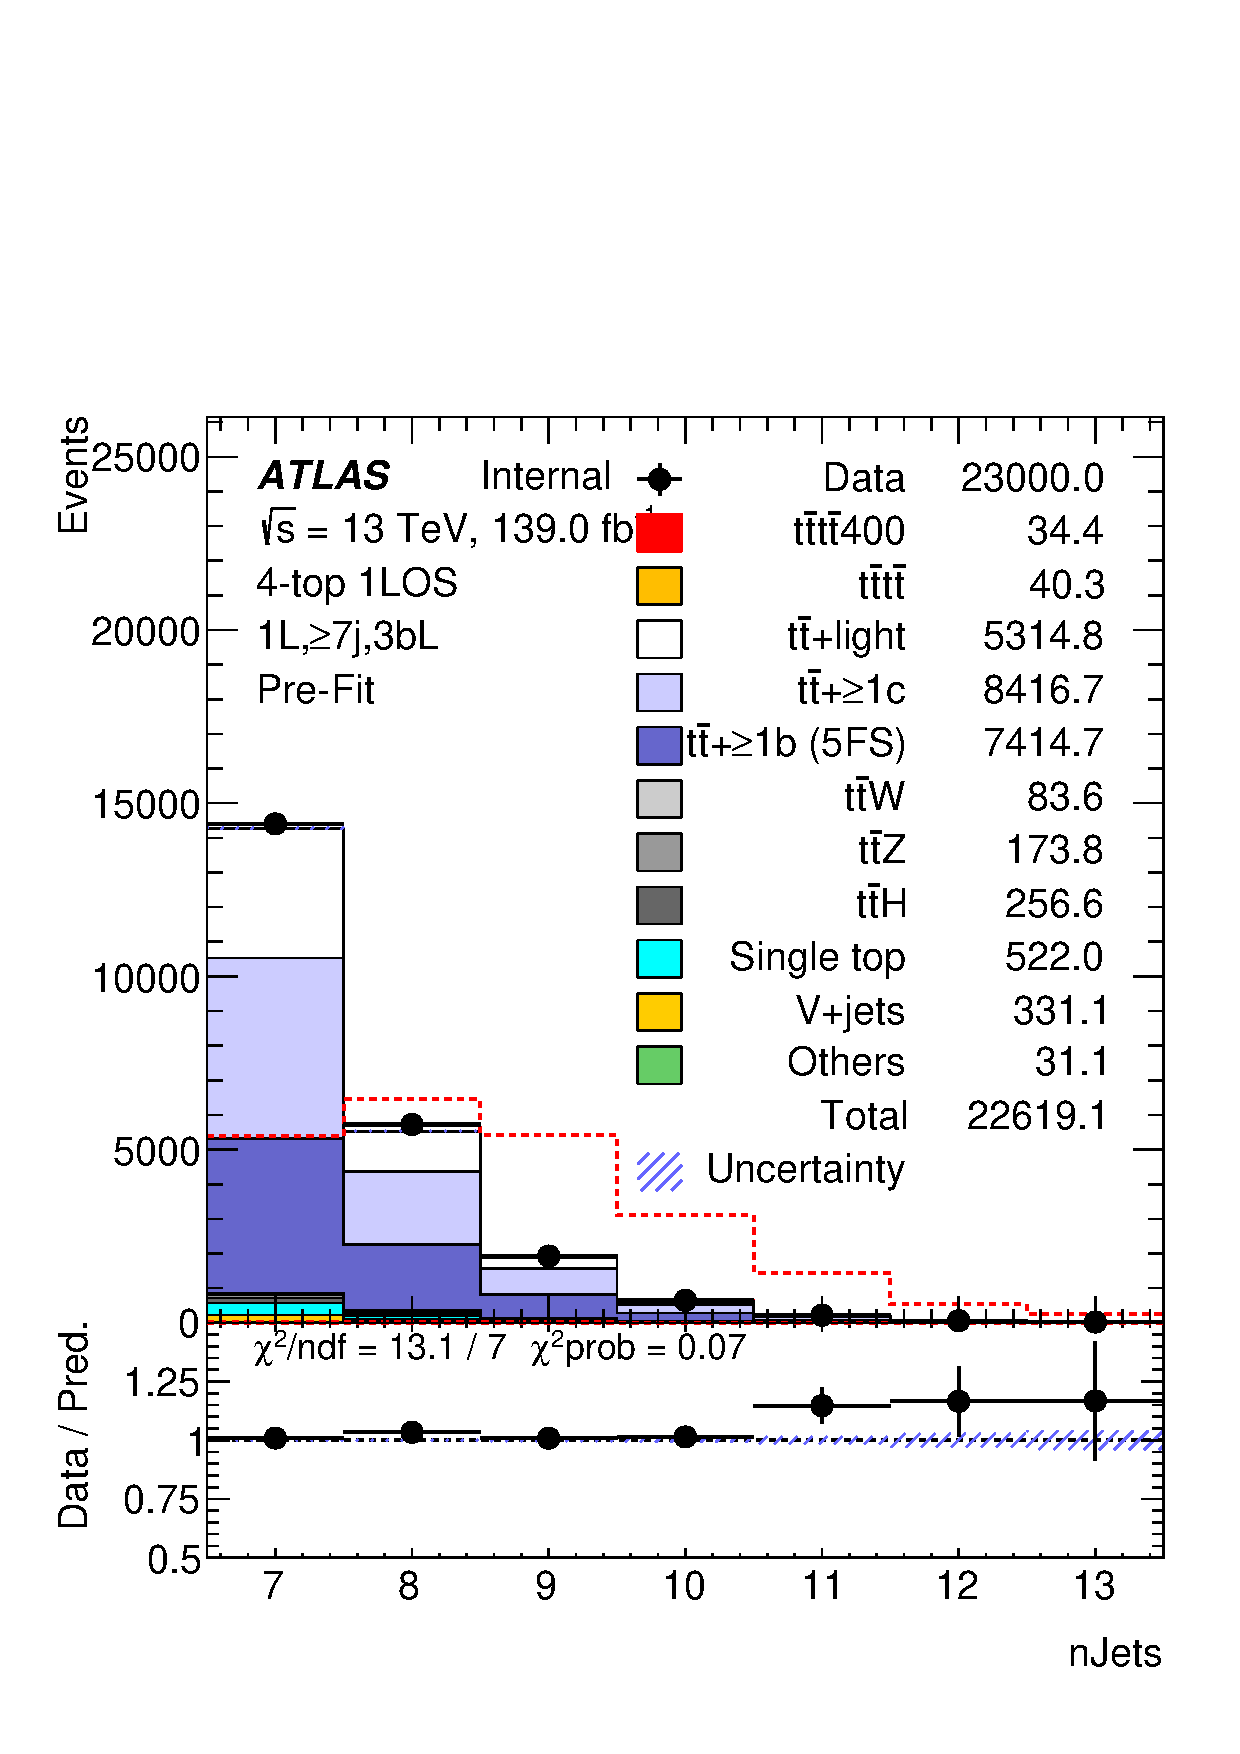
\includegraphics[width=0.25 \textwidth]{figures/fits/4FSvs5FS/GNN/400/Data_to_MC_5FS/val_ljets_ge7j3bL.pdf}&
      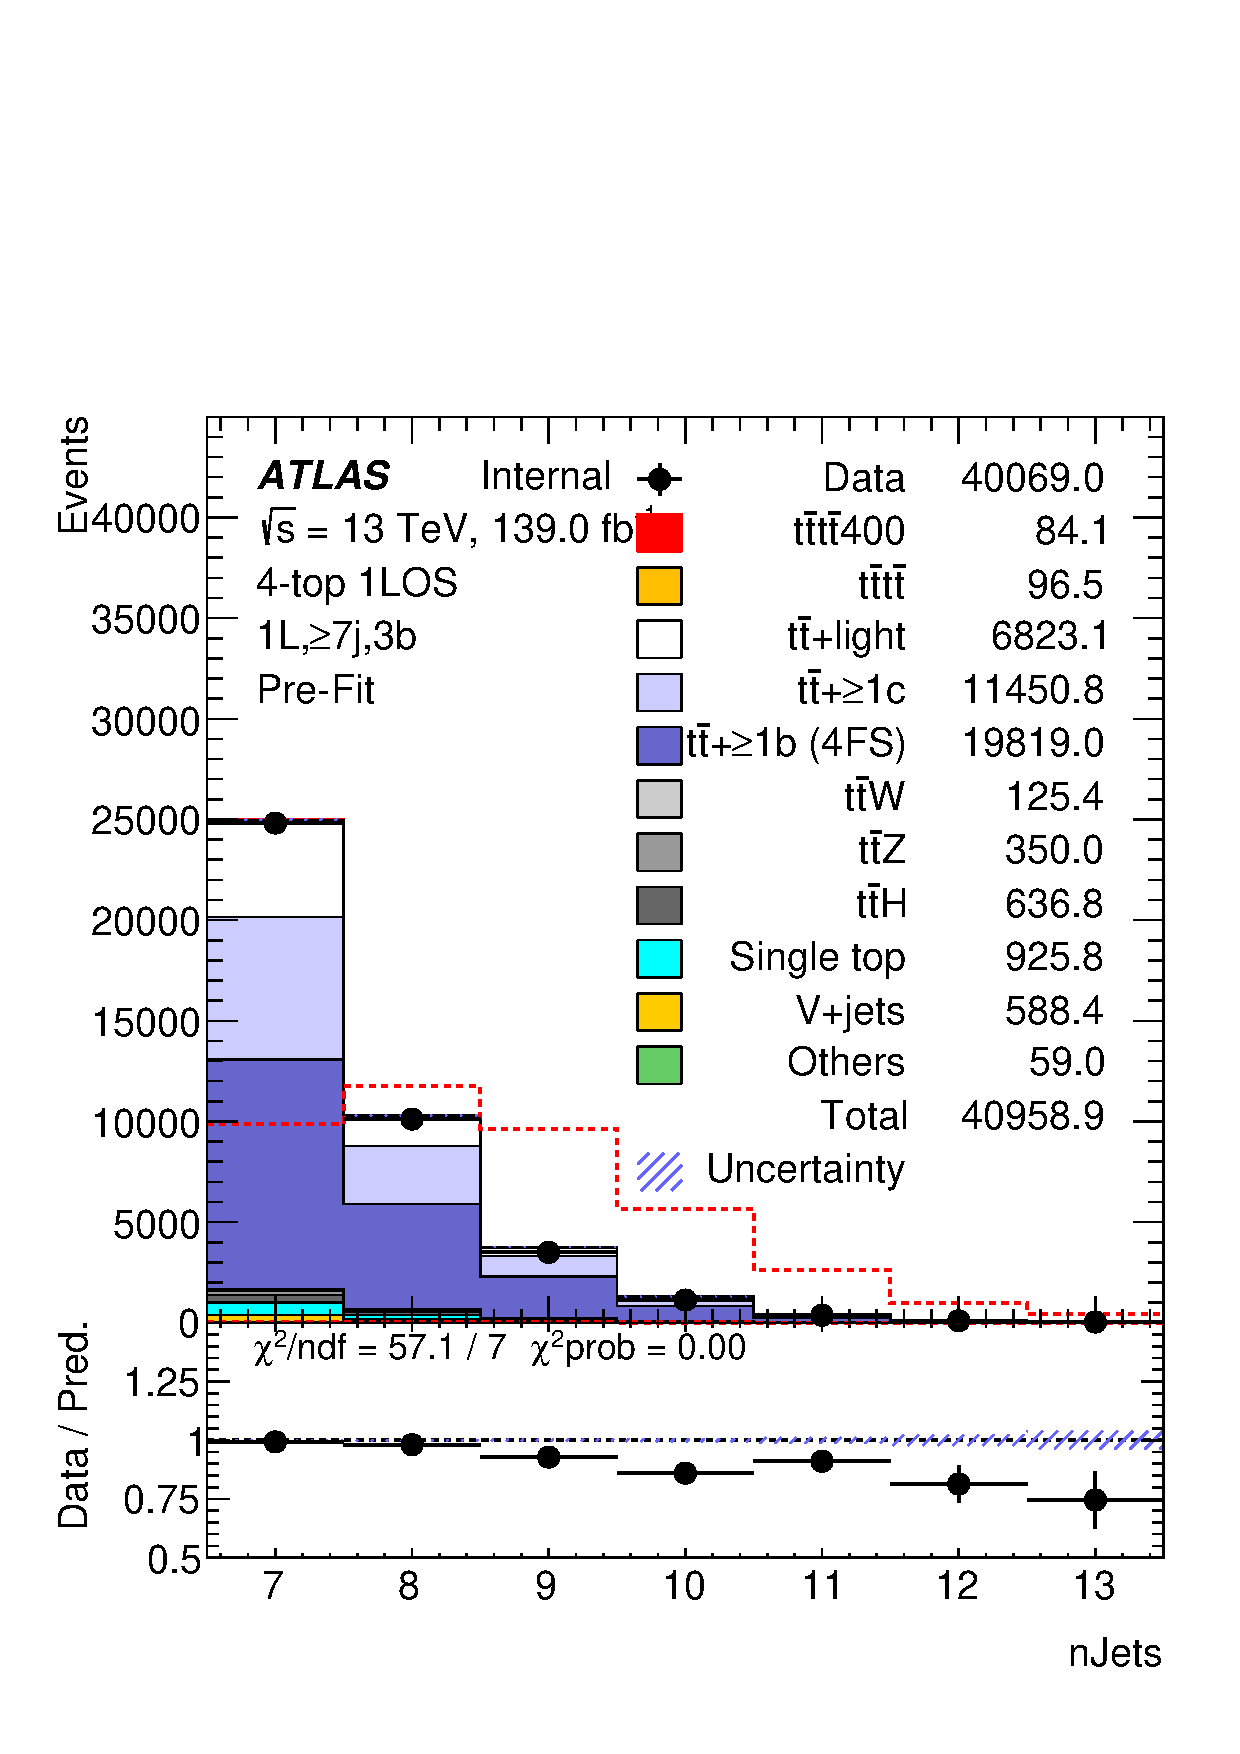
\includegraphics[width=0.25 \textwidth]{figures/fits/4FSvs5FS/GNN/400/Data_to_MC_4FS/val_ljets_ge7j3b.pdf} &                                                                      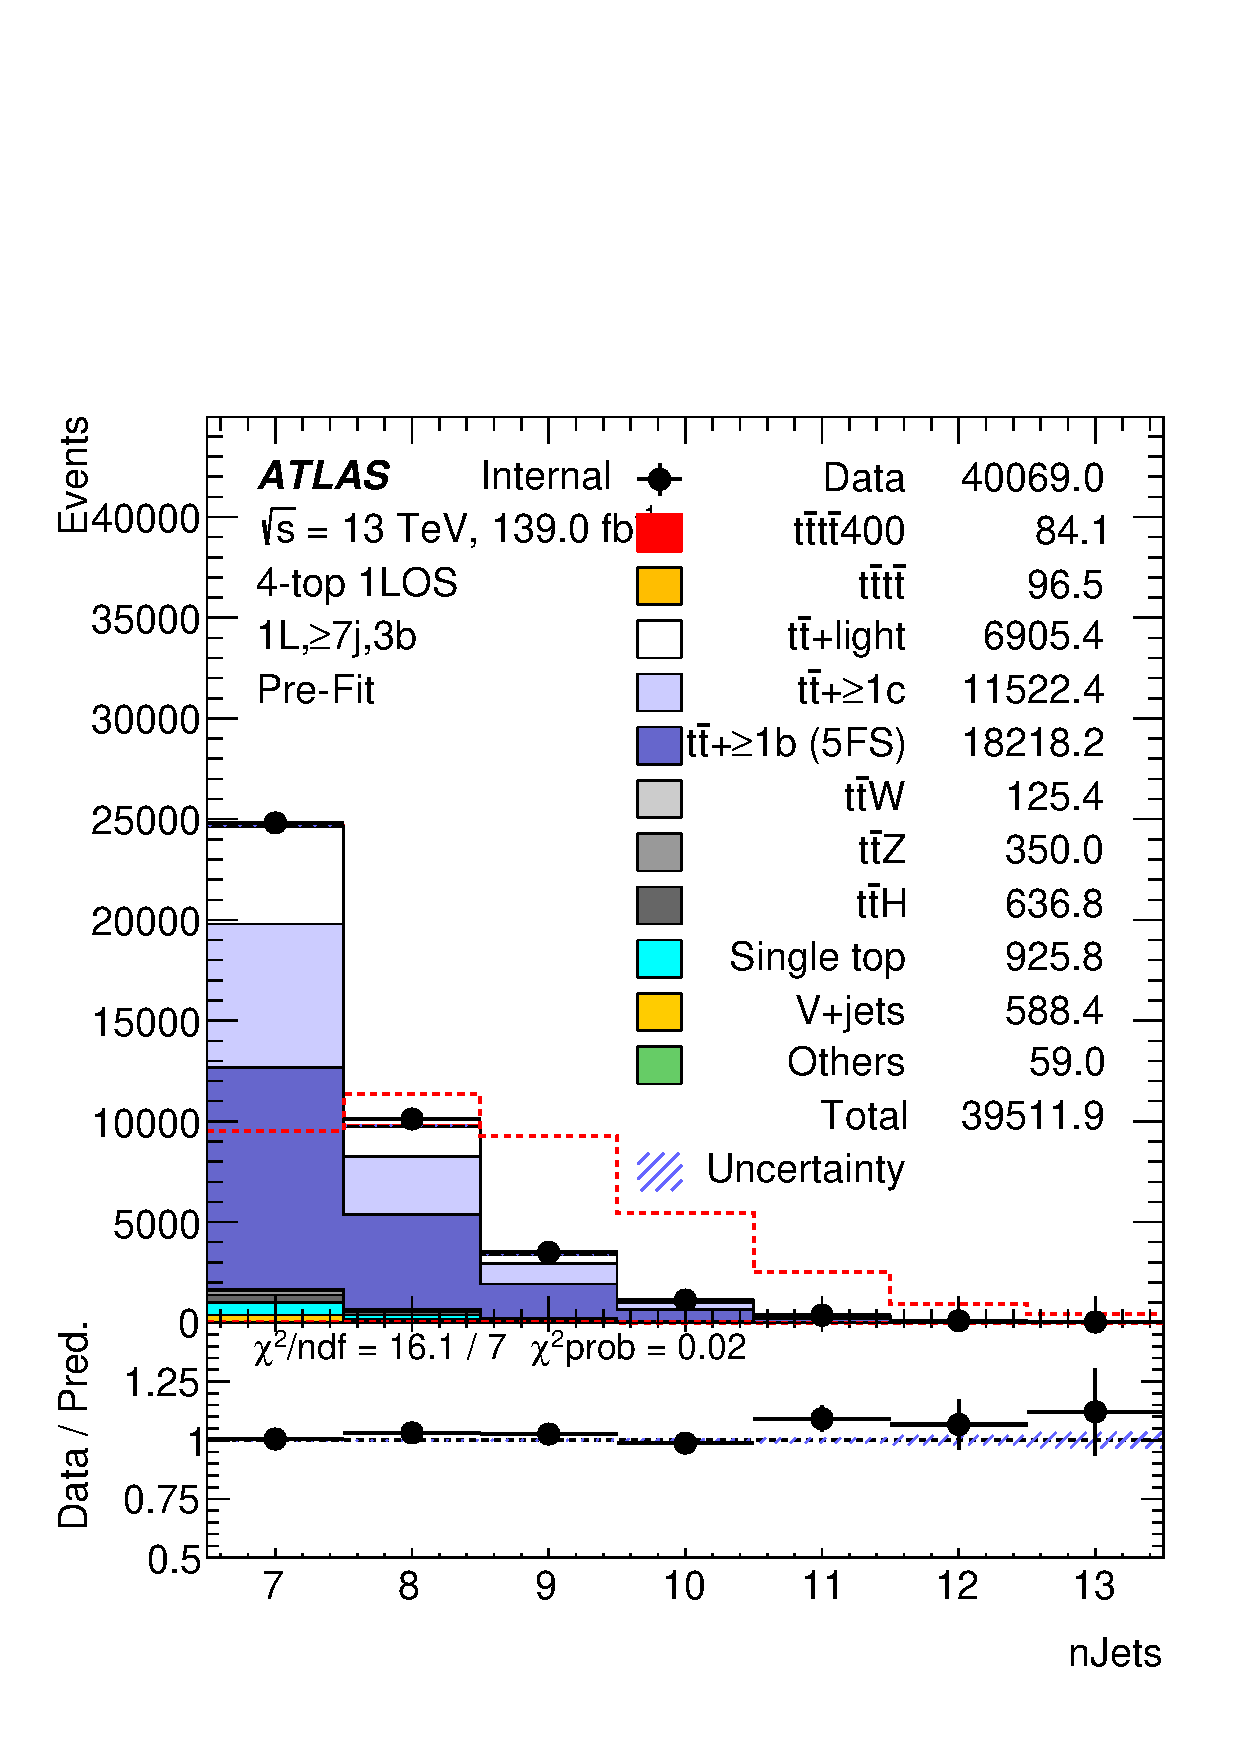
\includegraphics[width=0.25 \textwidth]{figures/fits/4FSvs5FS/GNN/400/Data_to_MC_5FS/val_ljets_ge7j3b.pdf}\\

      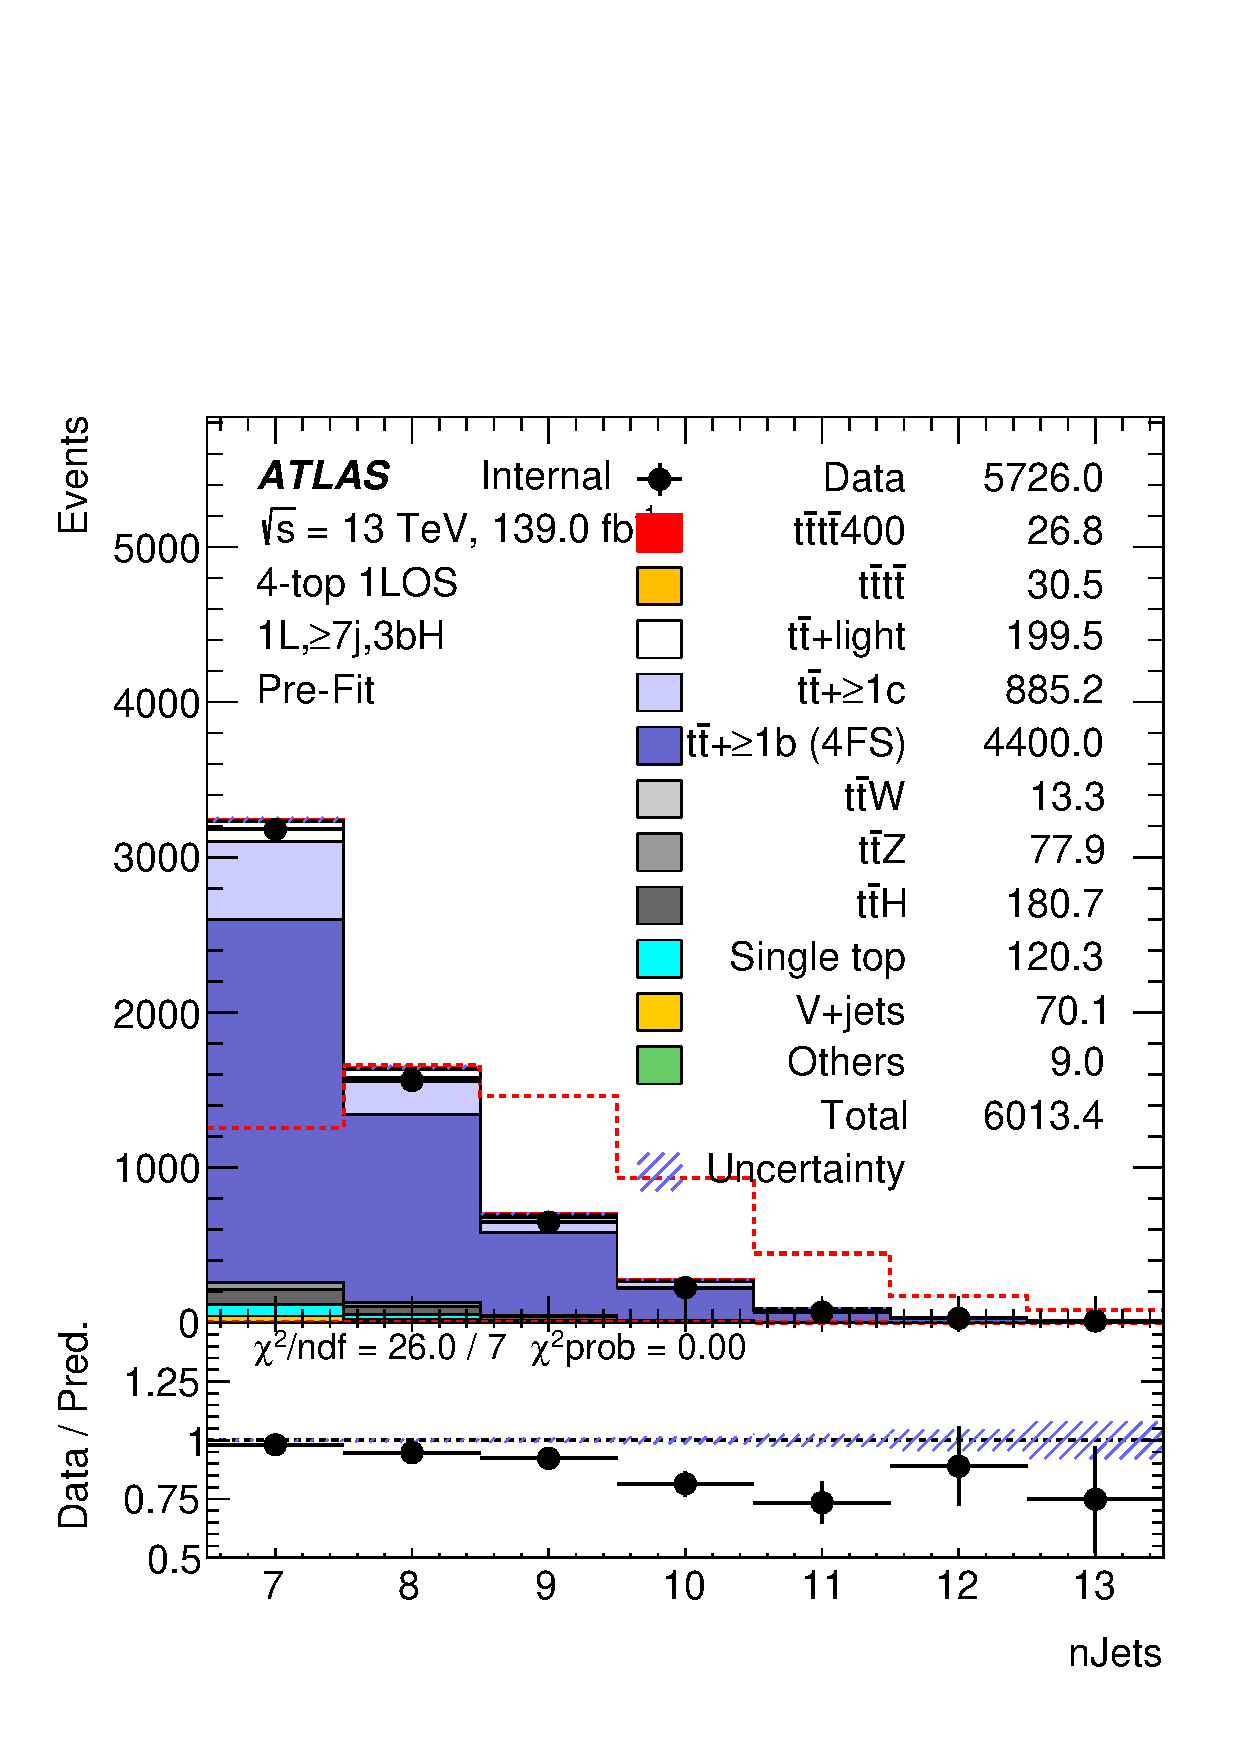
\includegraphics[width=0.25 \textwidth]{figures/fits/4FSvs5FS/GNN/400/Data_to_MC_4FS/val_ljets_ge7j3bH.pdf} &                                                                     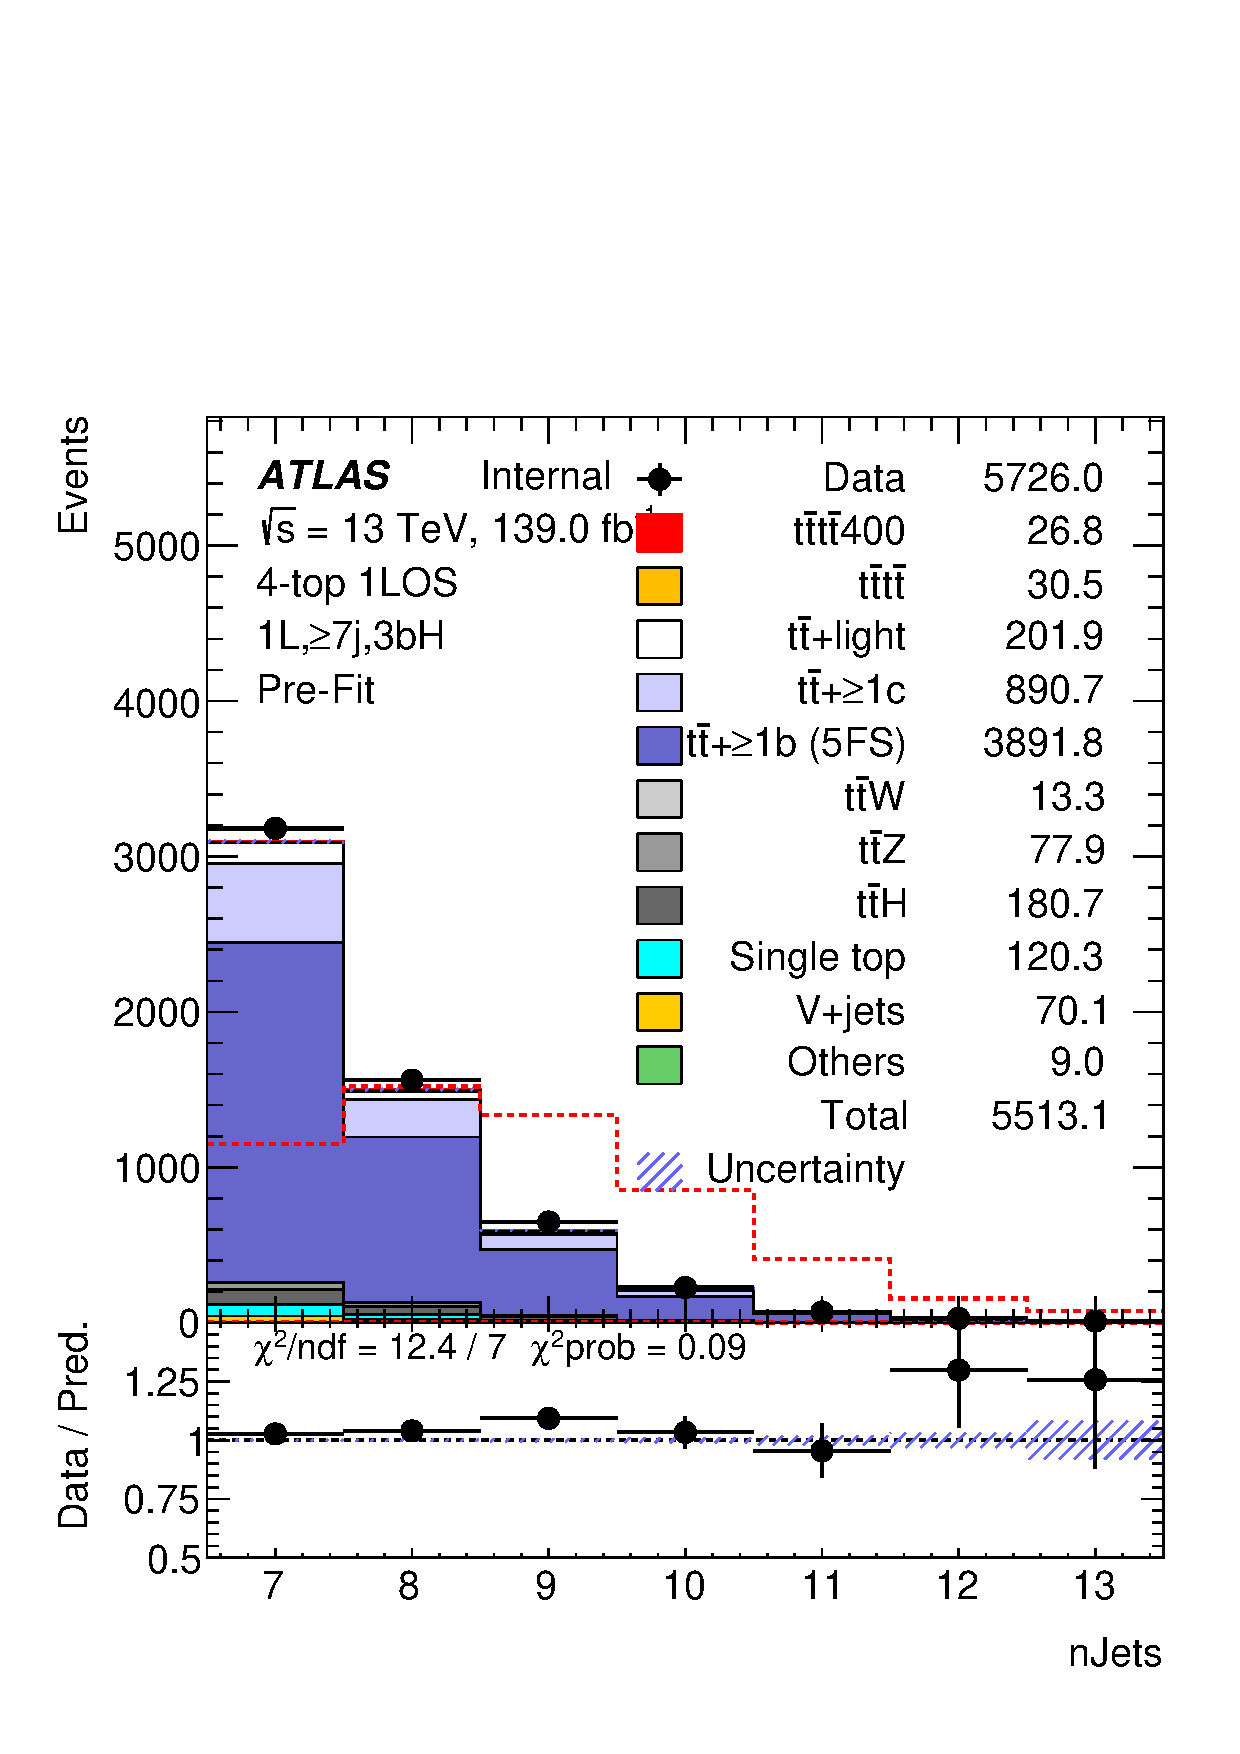
\includegraphics[width=0.25 \textwidth]{figures/fits/4FSvs5FS/GNN/400/Data_to_MC_5FS/val_ljets_ge7j3bH.pdf}&                                                              
      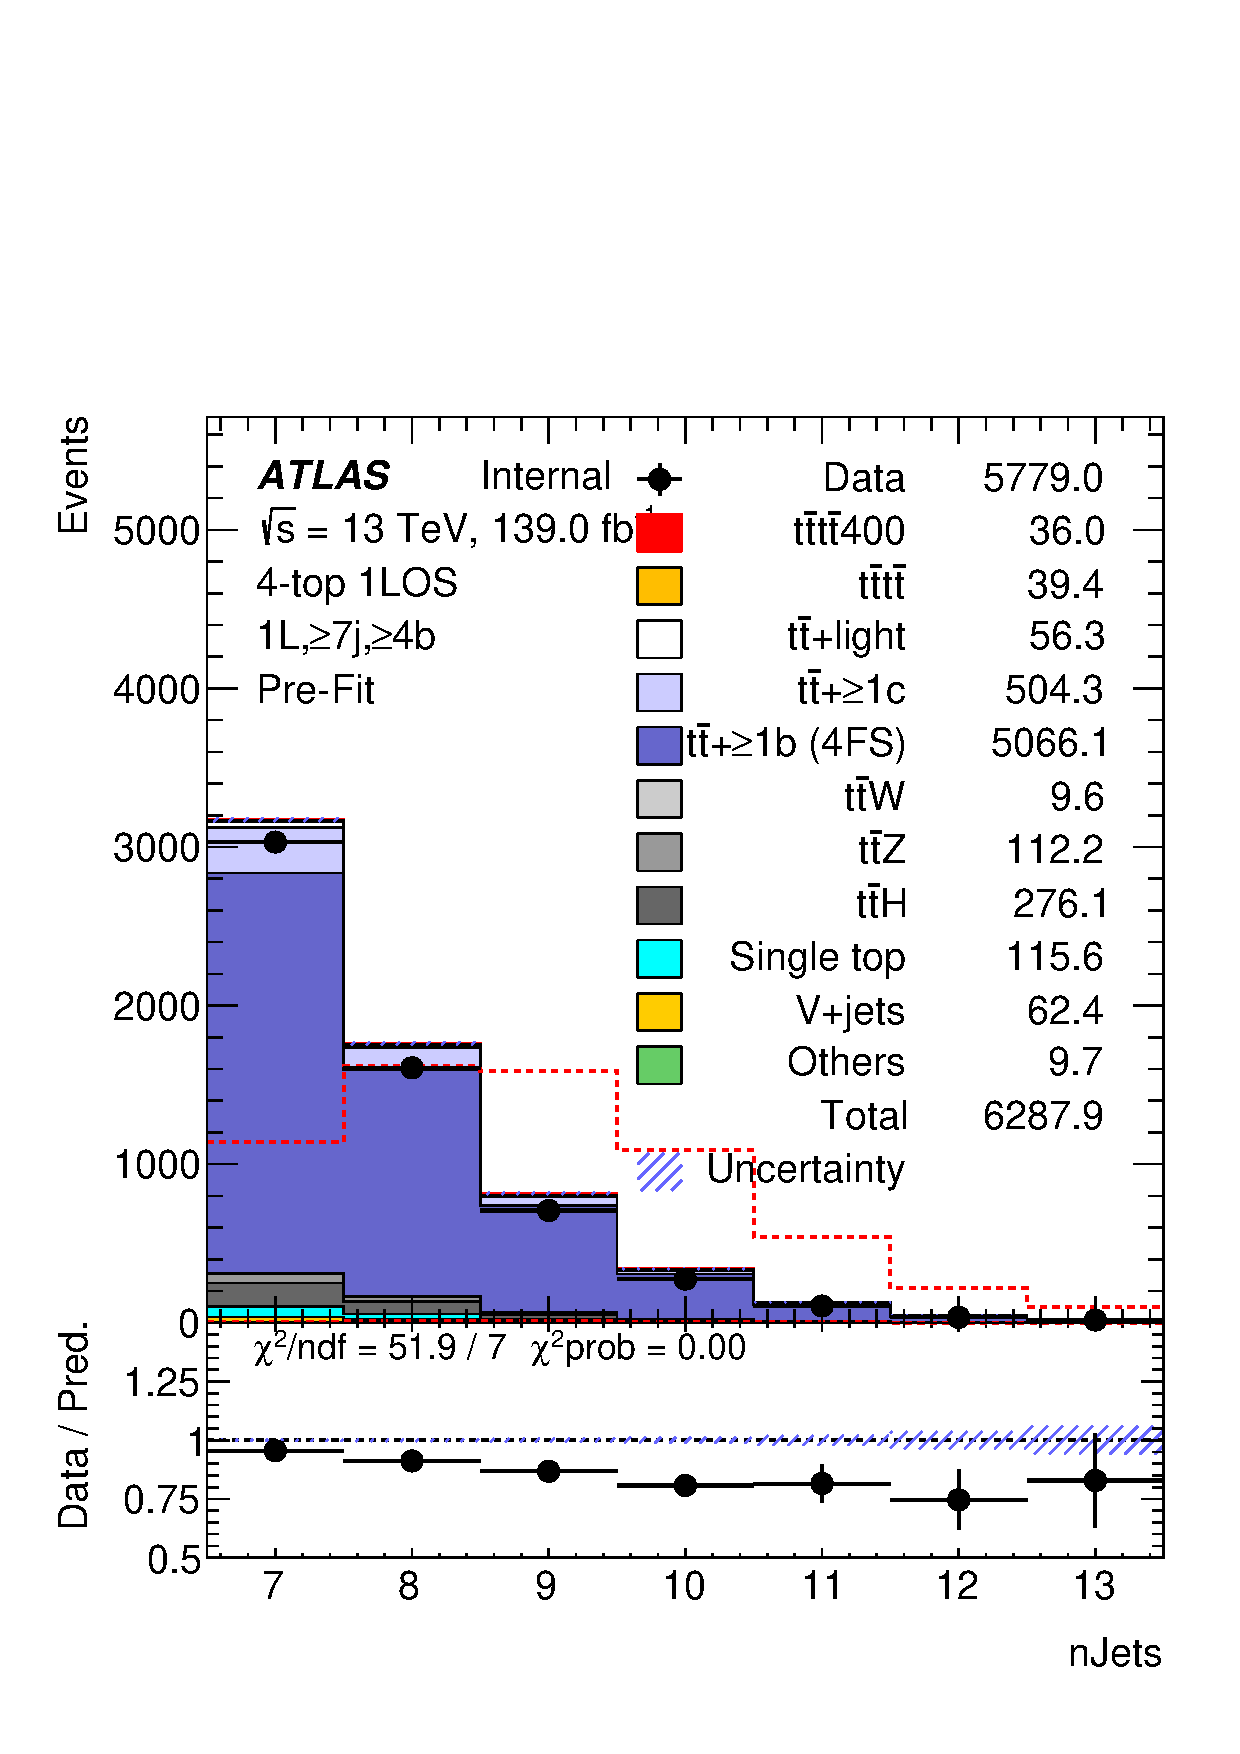
\includegraphics[width=0.25 \textwidth]{figures/fits/4FSvs5FS/GNN/400/Data_to_MC_4FS/val_ljets_ge7jge4b.pdf} &                                                              
      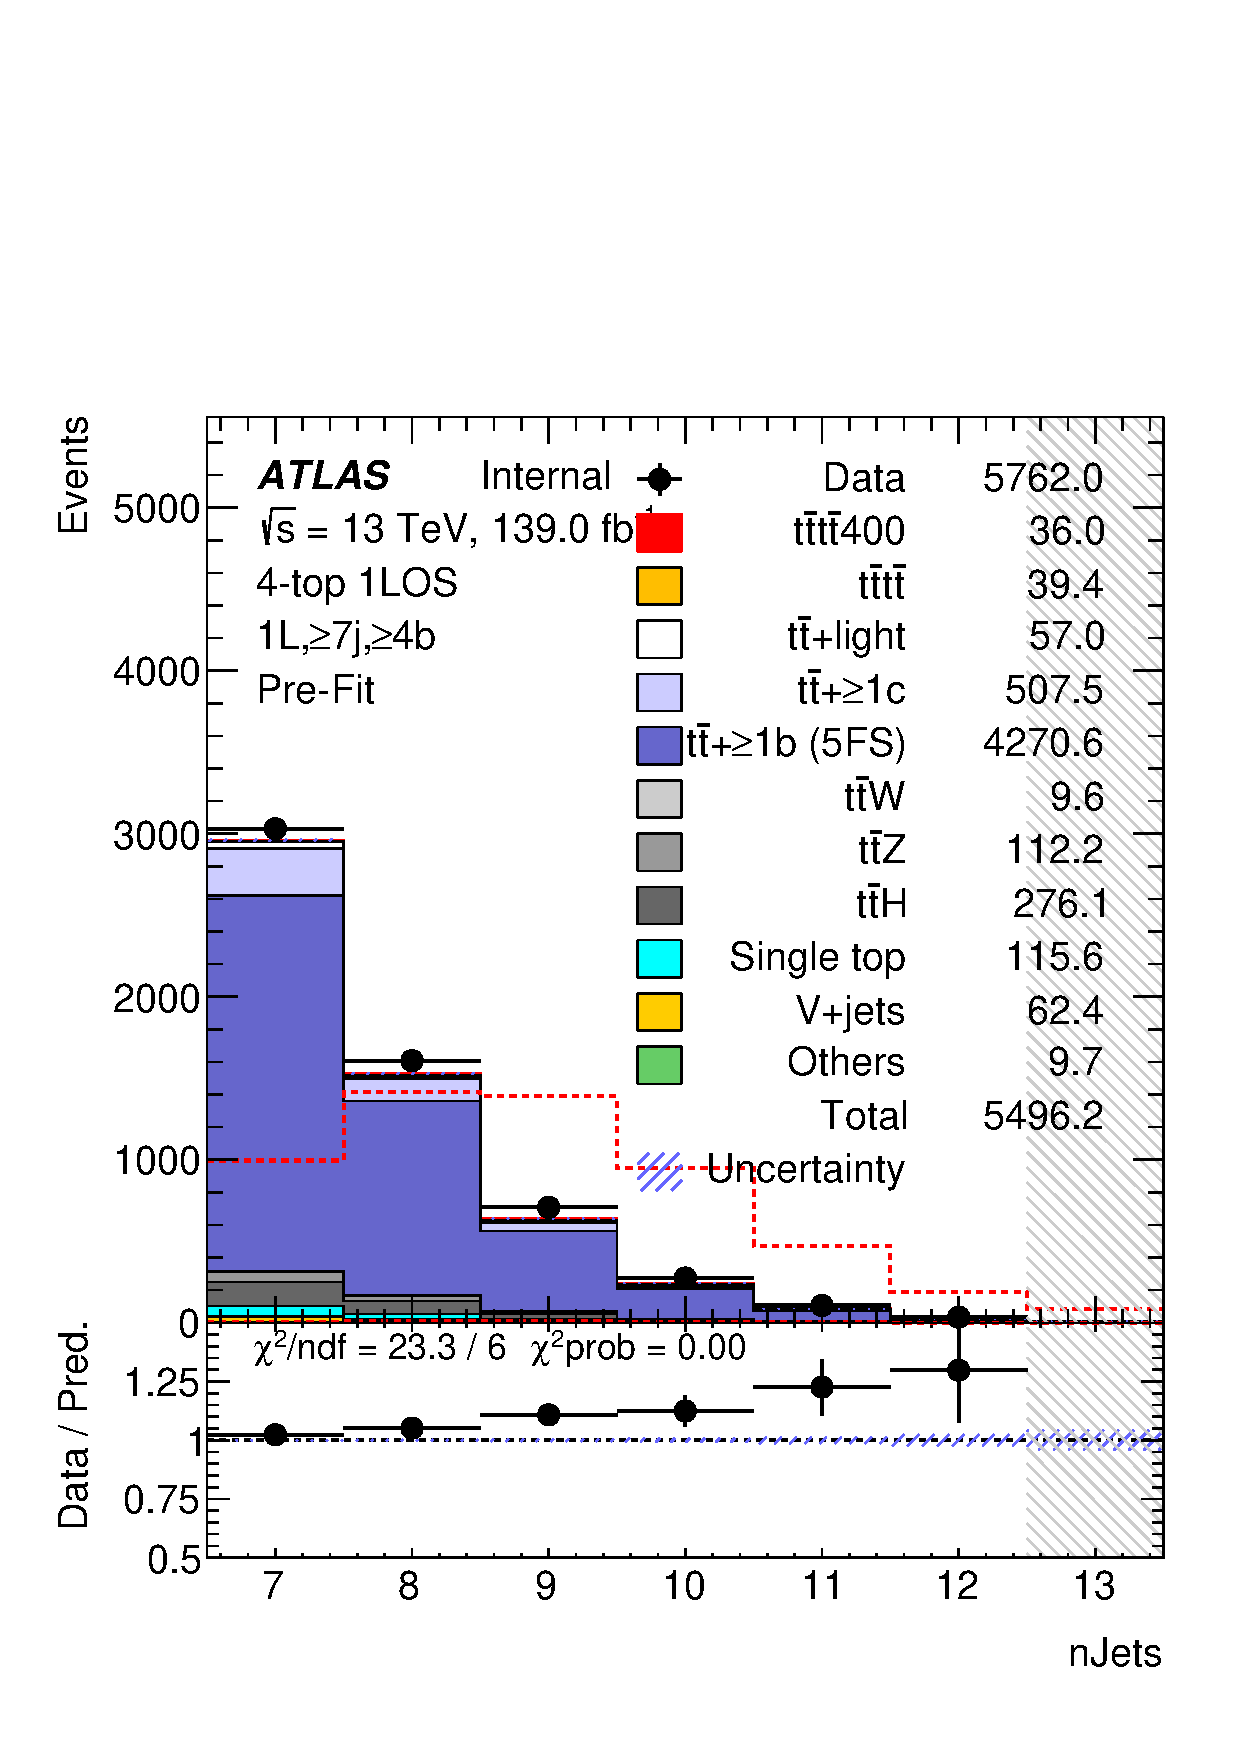
\includegraphics[width=0.25 \textwidth]{figures/fits/4FSvs5FS/GNN/400/Data_to_MC_5FS/val_ljets_ge7jge4b.pdf}\\                                                             

      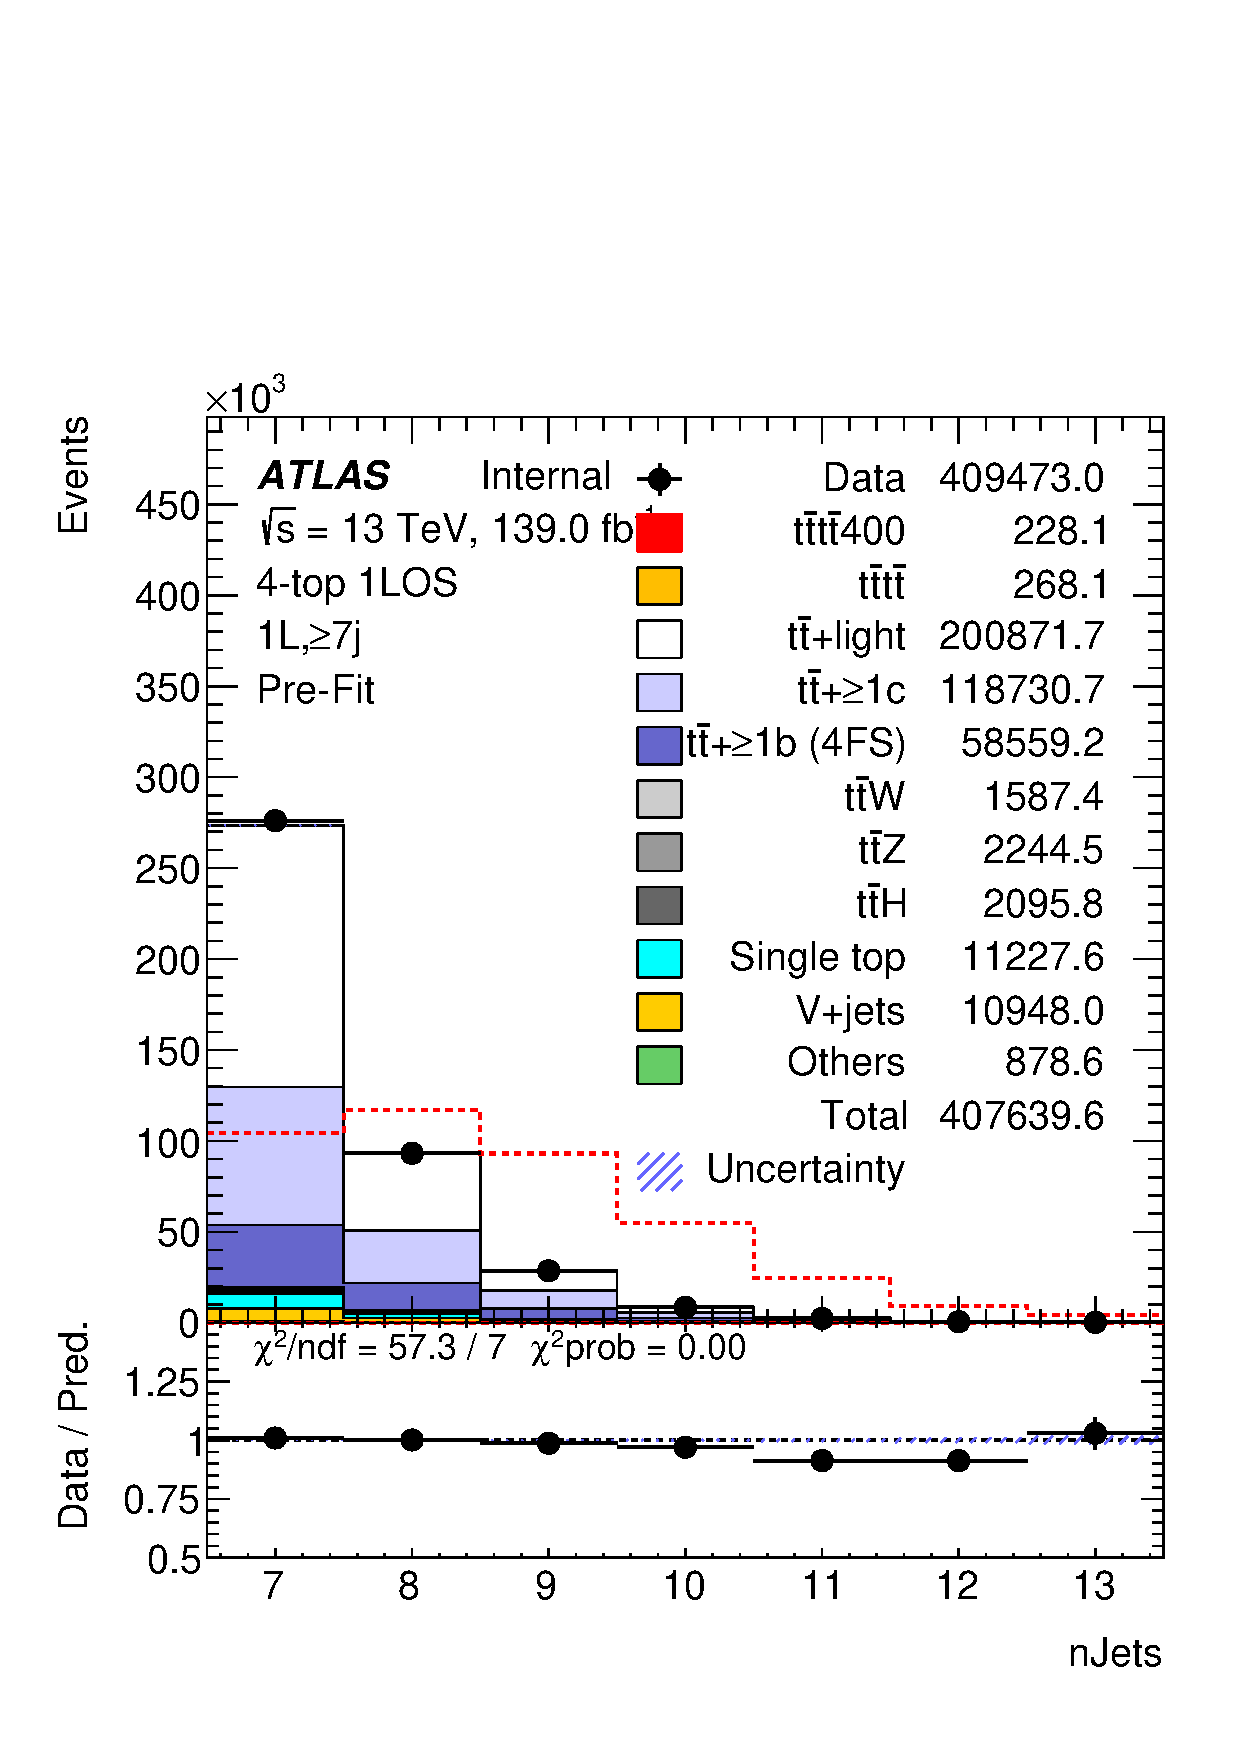
\includegraphics[width=0.25 \textwidth]{figures/fits/4FSvs5FS/GNN/400/Data_to_MC_4FS/val_ljets_ge7j.pdf} &                                                                  
      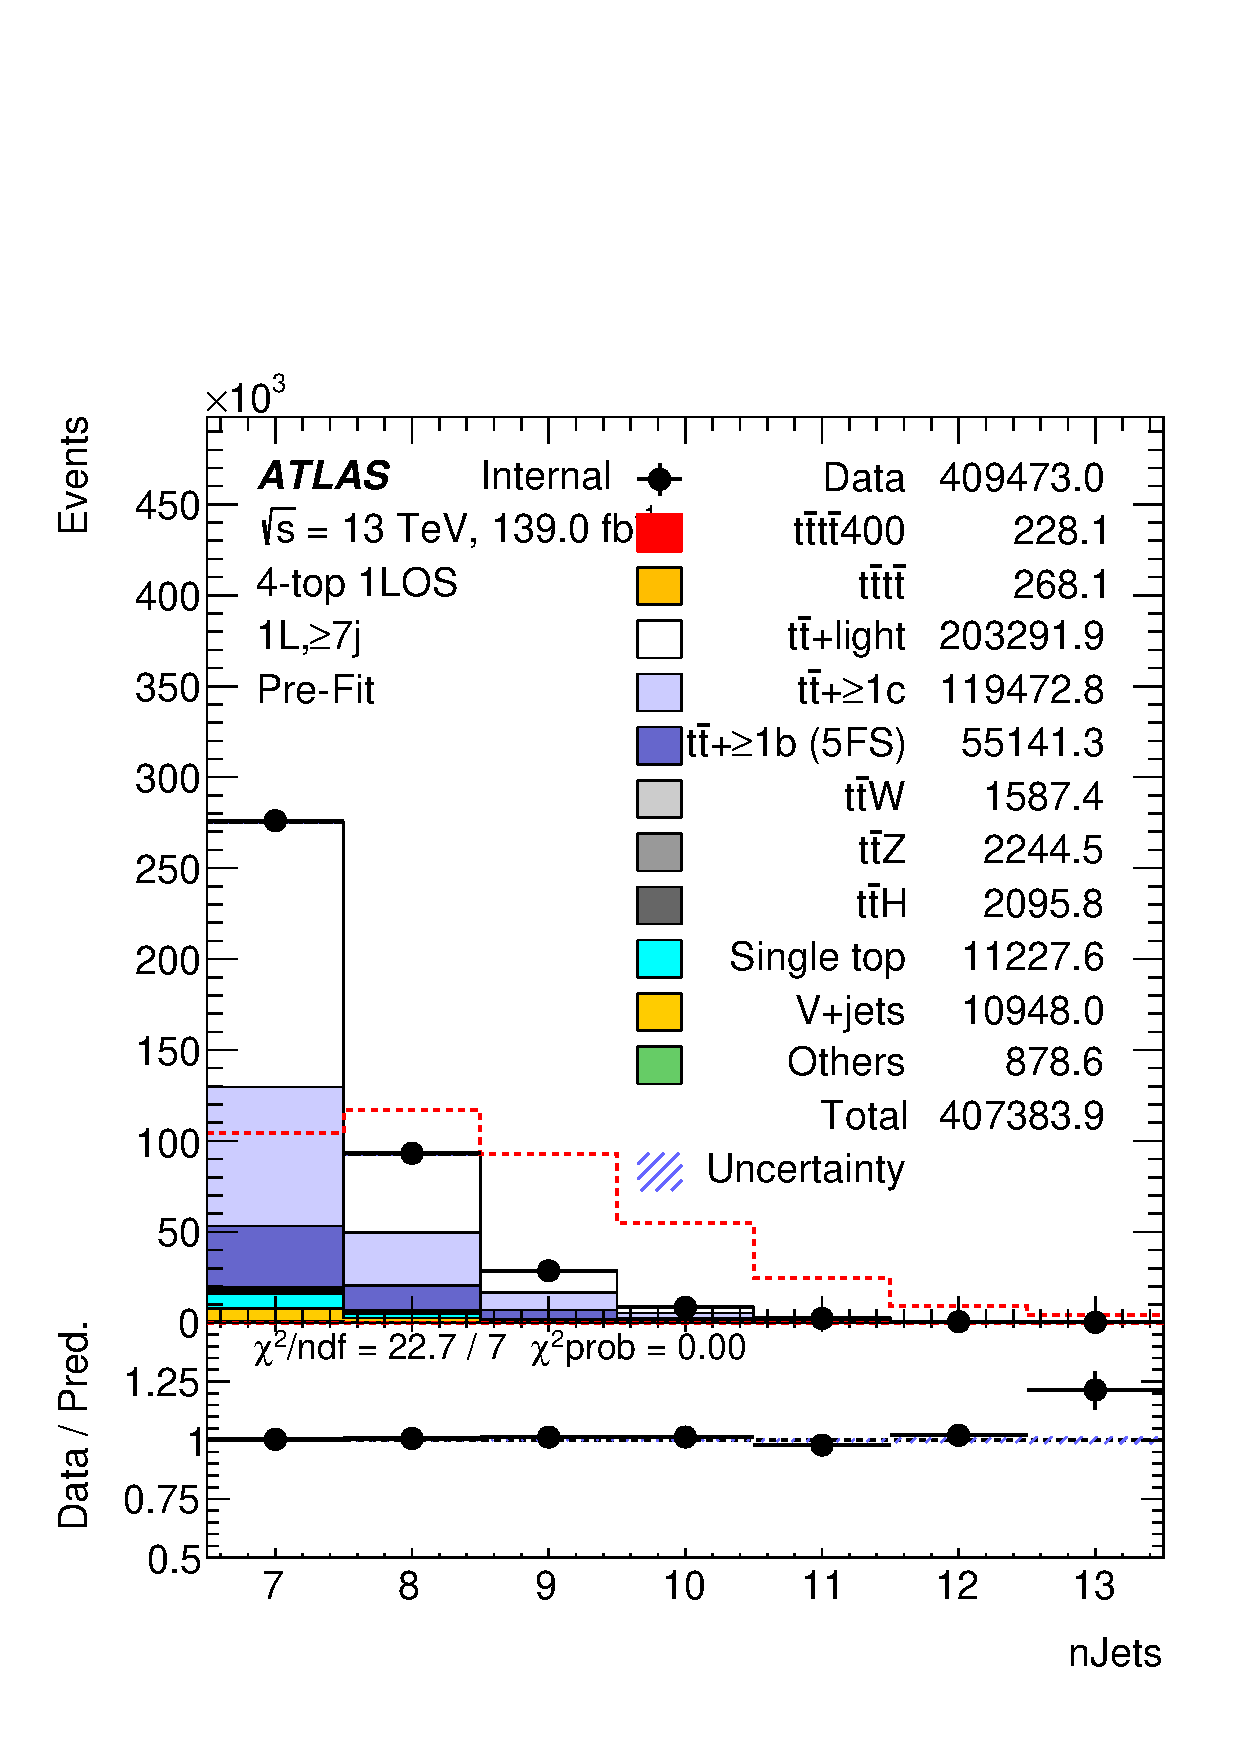
\includegraphics[width=0.25 \textwidth]{figures/fits/4FSvs5FS/GNN/400/Data_to_MC_5FS/val_ljets_ge7j.pdf}\\                                                               

                                                                                                                                                                                      \end{tabular}                                                                                                                                                                  
\caption{\label{4FSvs5FS_dataMC_nJets}Pre-fit distributions in 5FS compared with 4FS for 1L channel associated with different signal and background samples, compared with data yields in the Njets distribution.}                                                                                                                                                                            
\end{center}                                                                                                                                                                       
\end{figure}                                                                                                                                                                                   

                                                                                                                                                                        
\begin{figure}[htbp!]                                                                                                                                                            
\begin{center} \setlength{\tabcolsep}{2.5pt}\footnotesize                                                                                                                        
\begin{tabular}{cccc} 


                                                                                                                                                                                  
      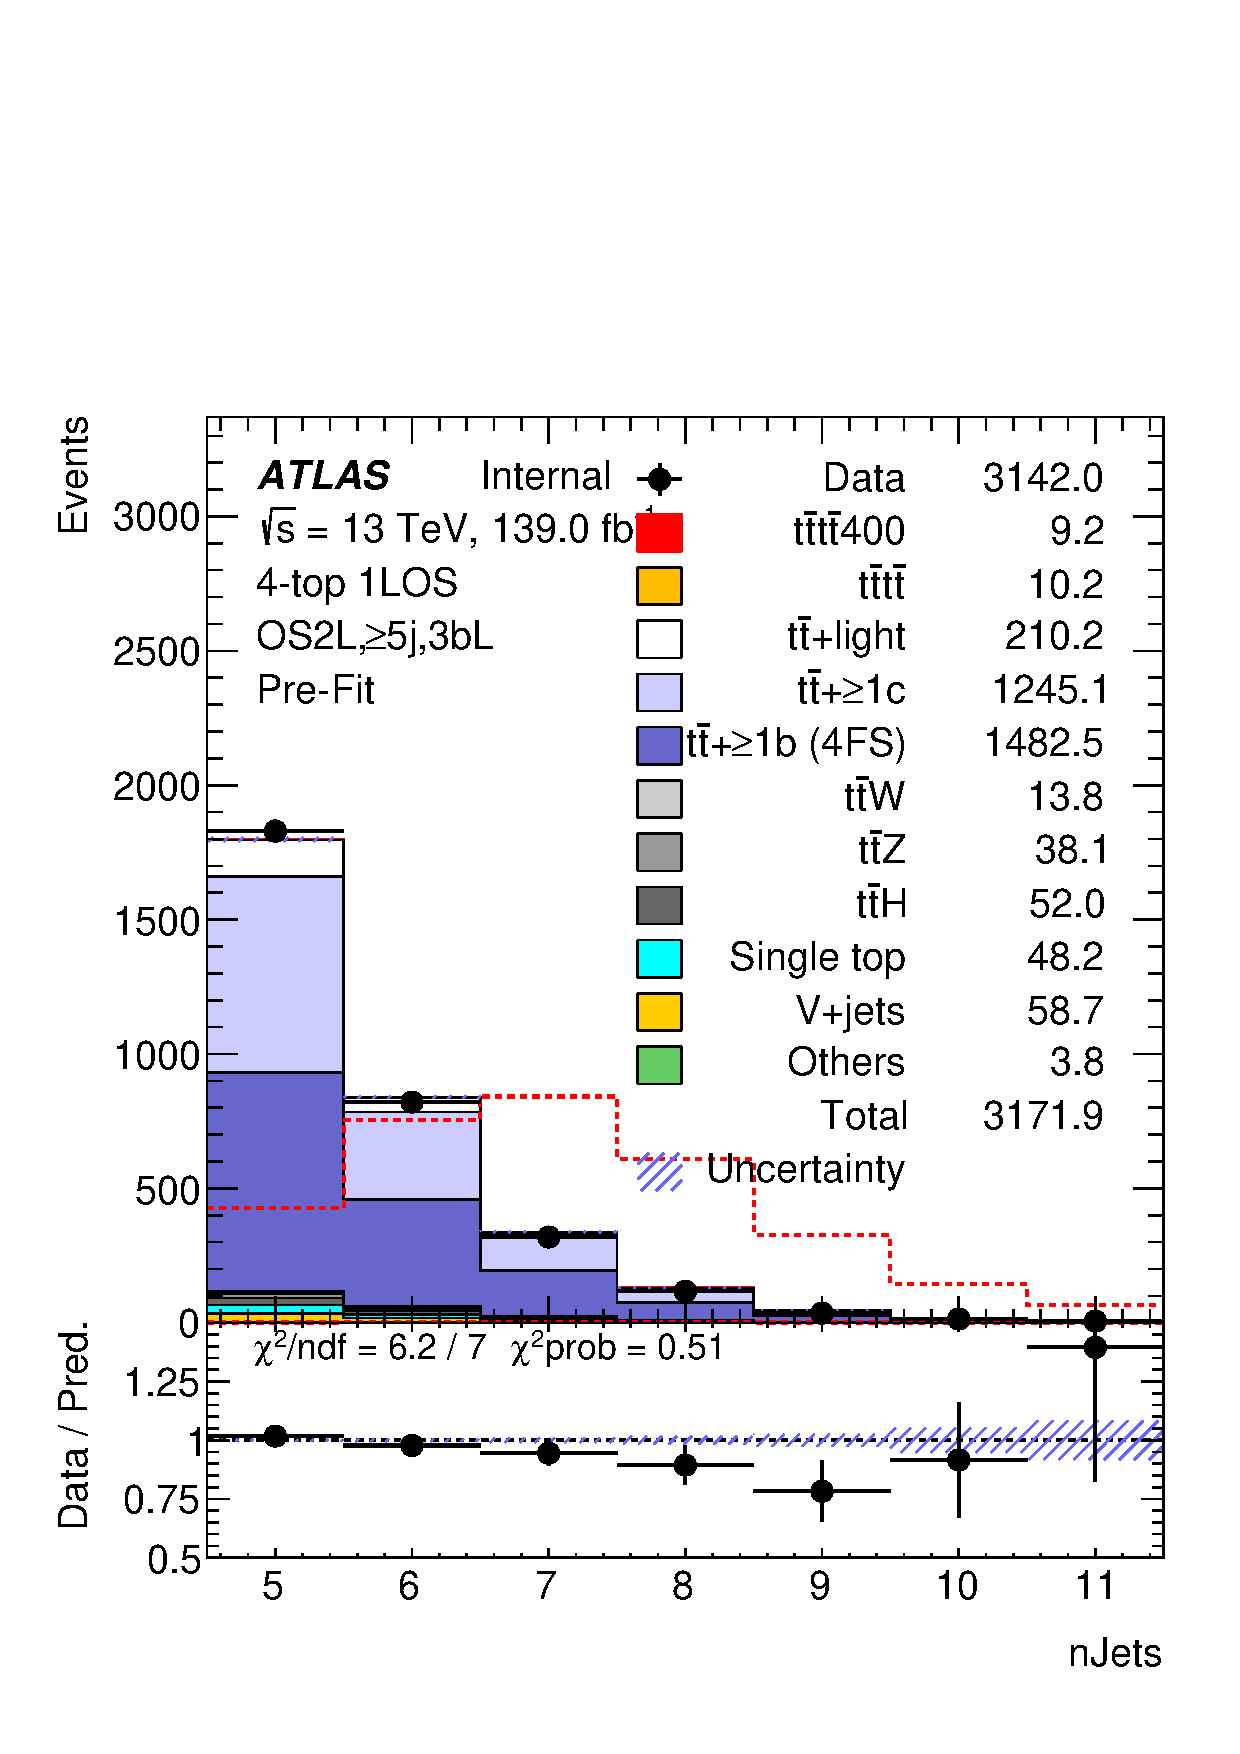
\includegraphics[width=0.25 \textwidth]{figures/fits/4FSvs5FS/GNN/400/Data_to_MC_4FS/val_os2l_ge5j3bL.pdf}&                                                                
      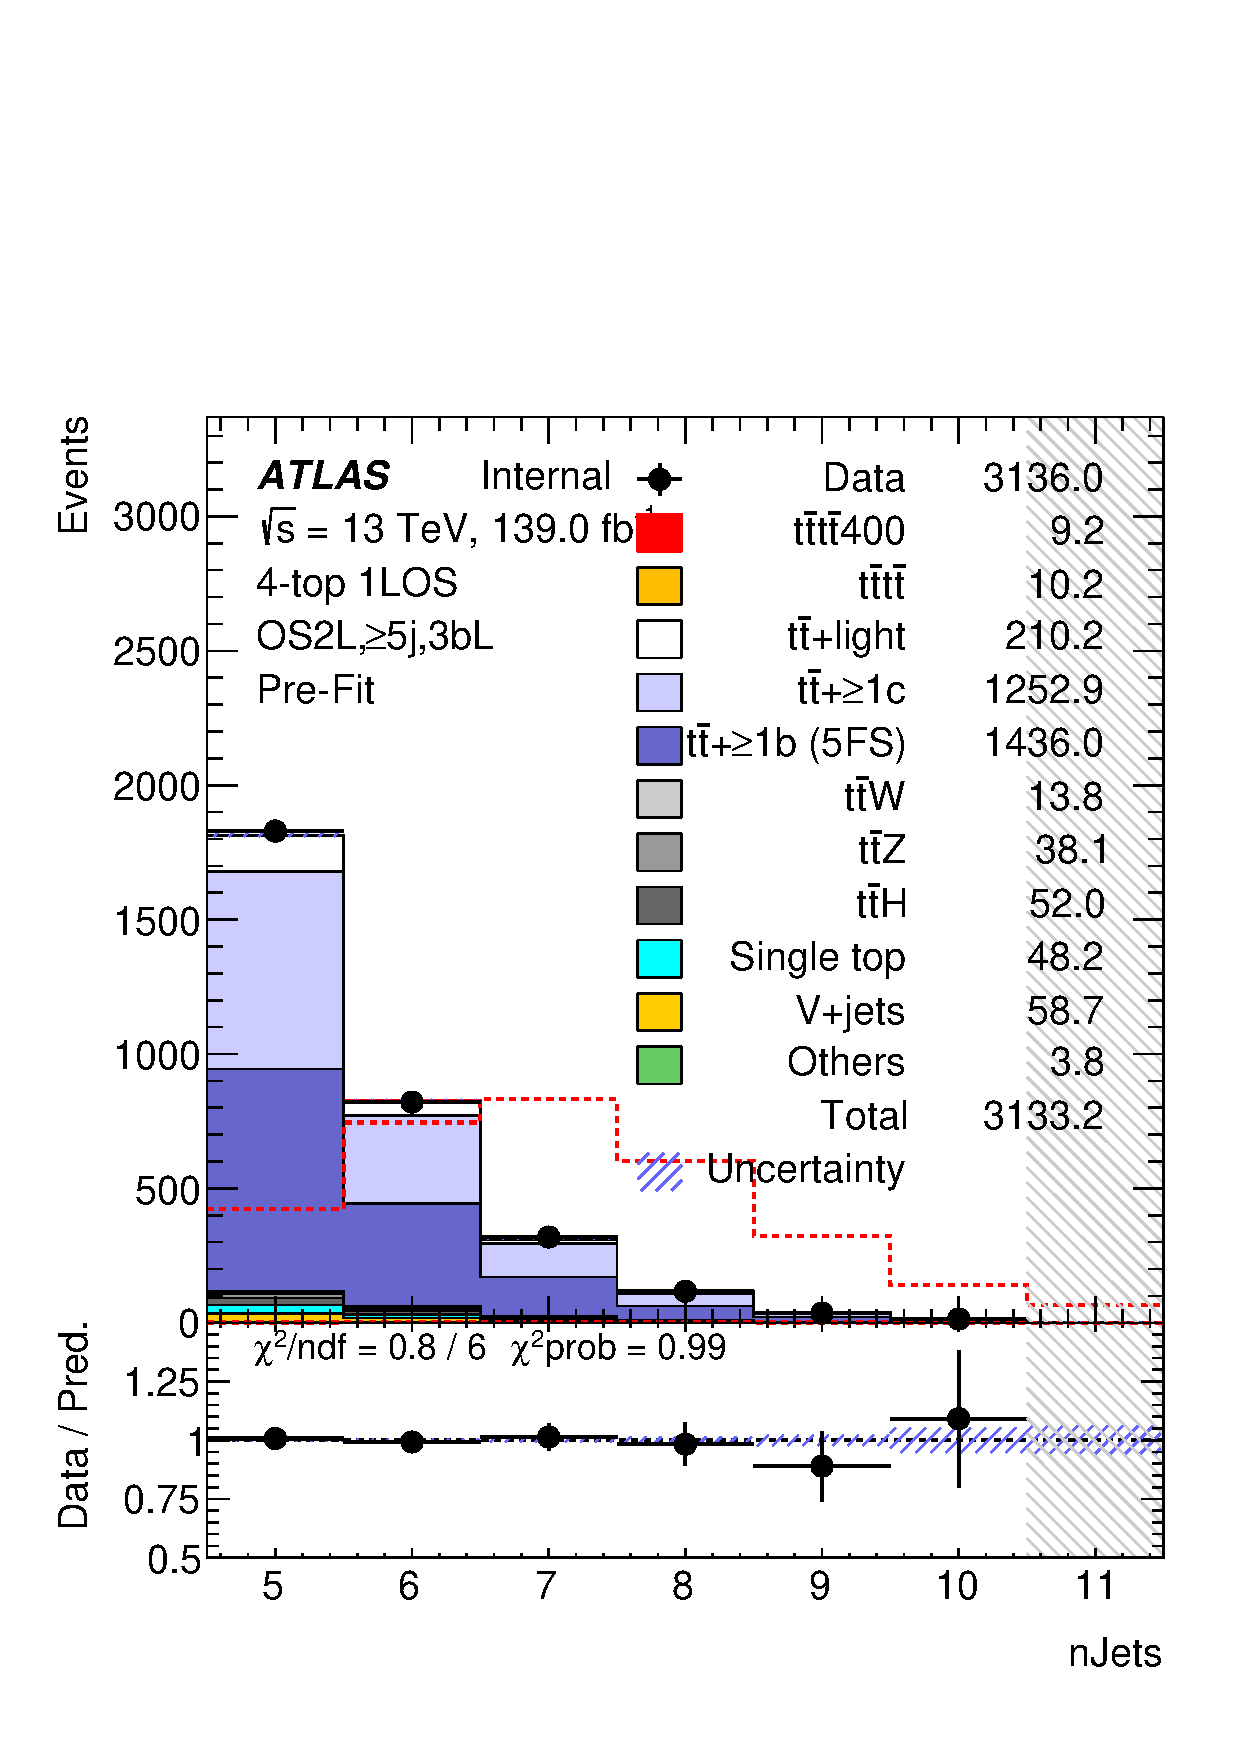
\includegraphics[width=0.25 \textwidth]{figures/fits/4FSvs5FS/GNN/400/Data_to_MC_5FS/val_os2l_ge5j3bL.pdf}&                                                                 
      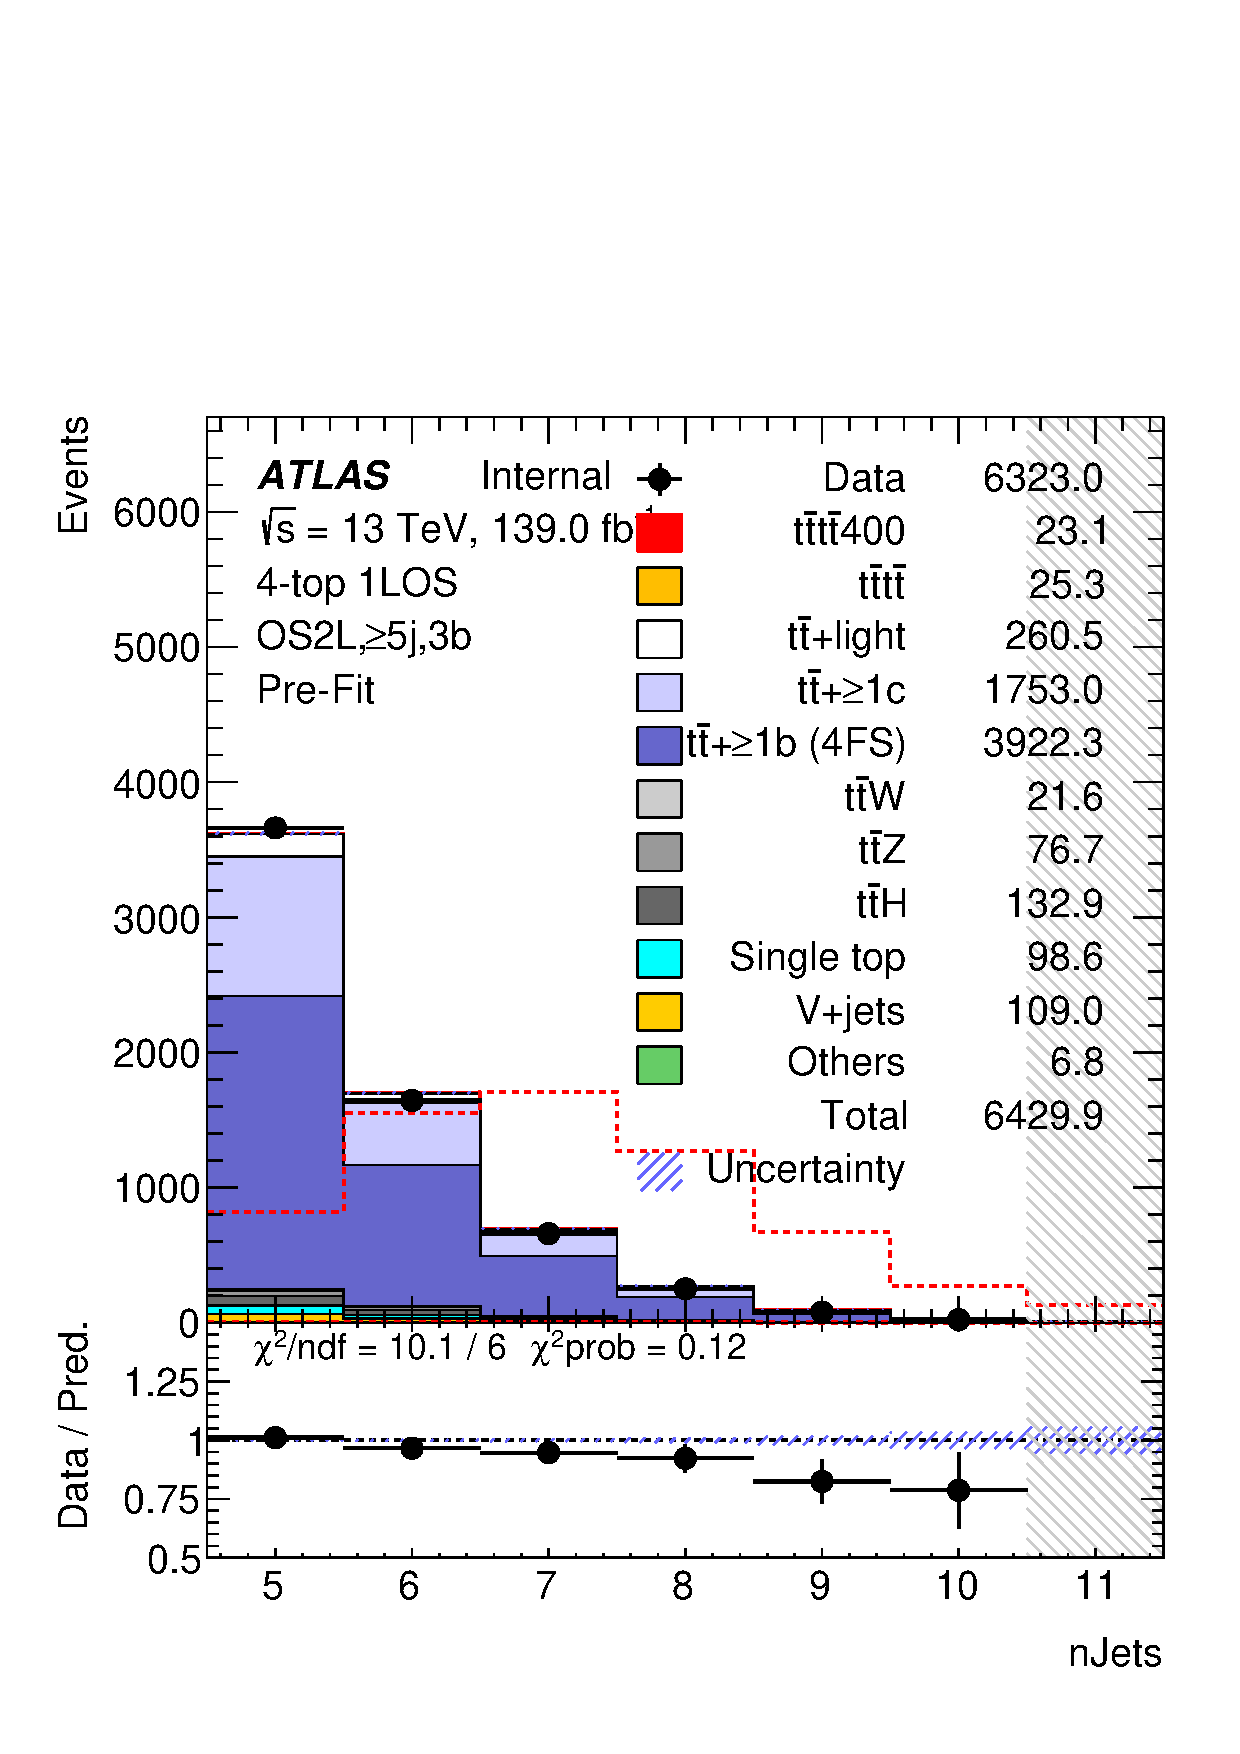
\includegraphics[width=0.25 \textwidth]{figures/fits/4FSvs5FS/GNN/400/Data_to_MC_4FS/val_os2l_ge5j3b.pdf}&
      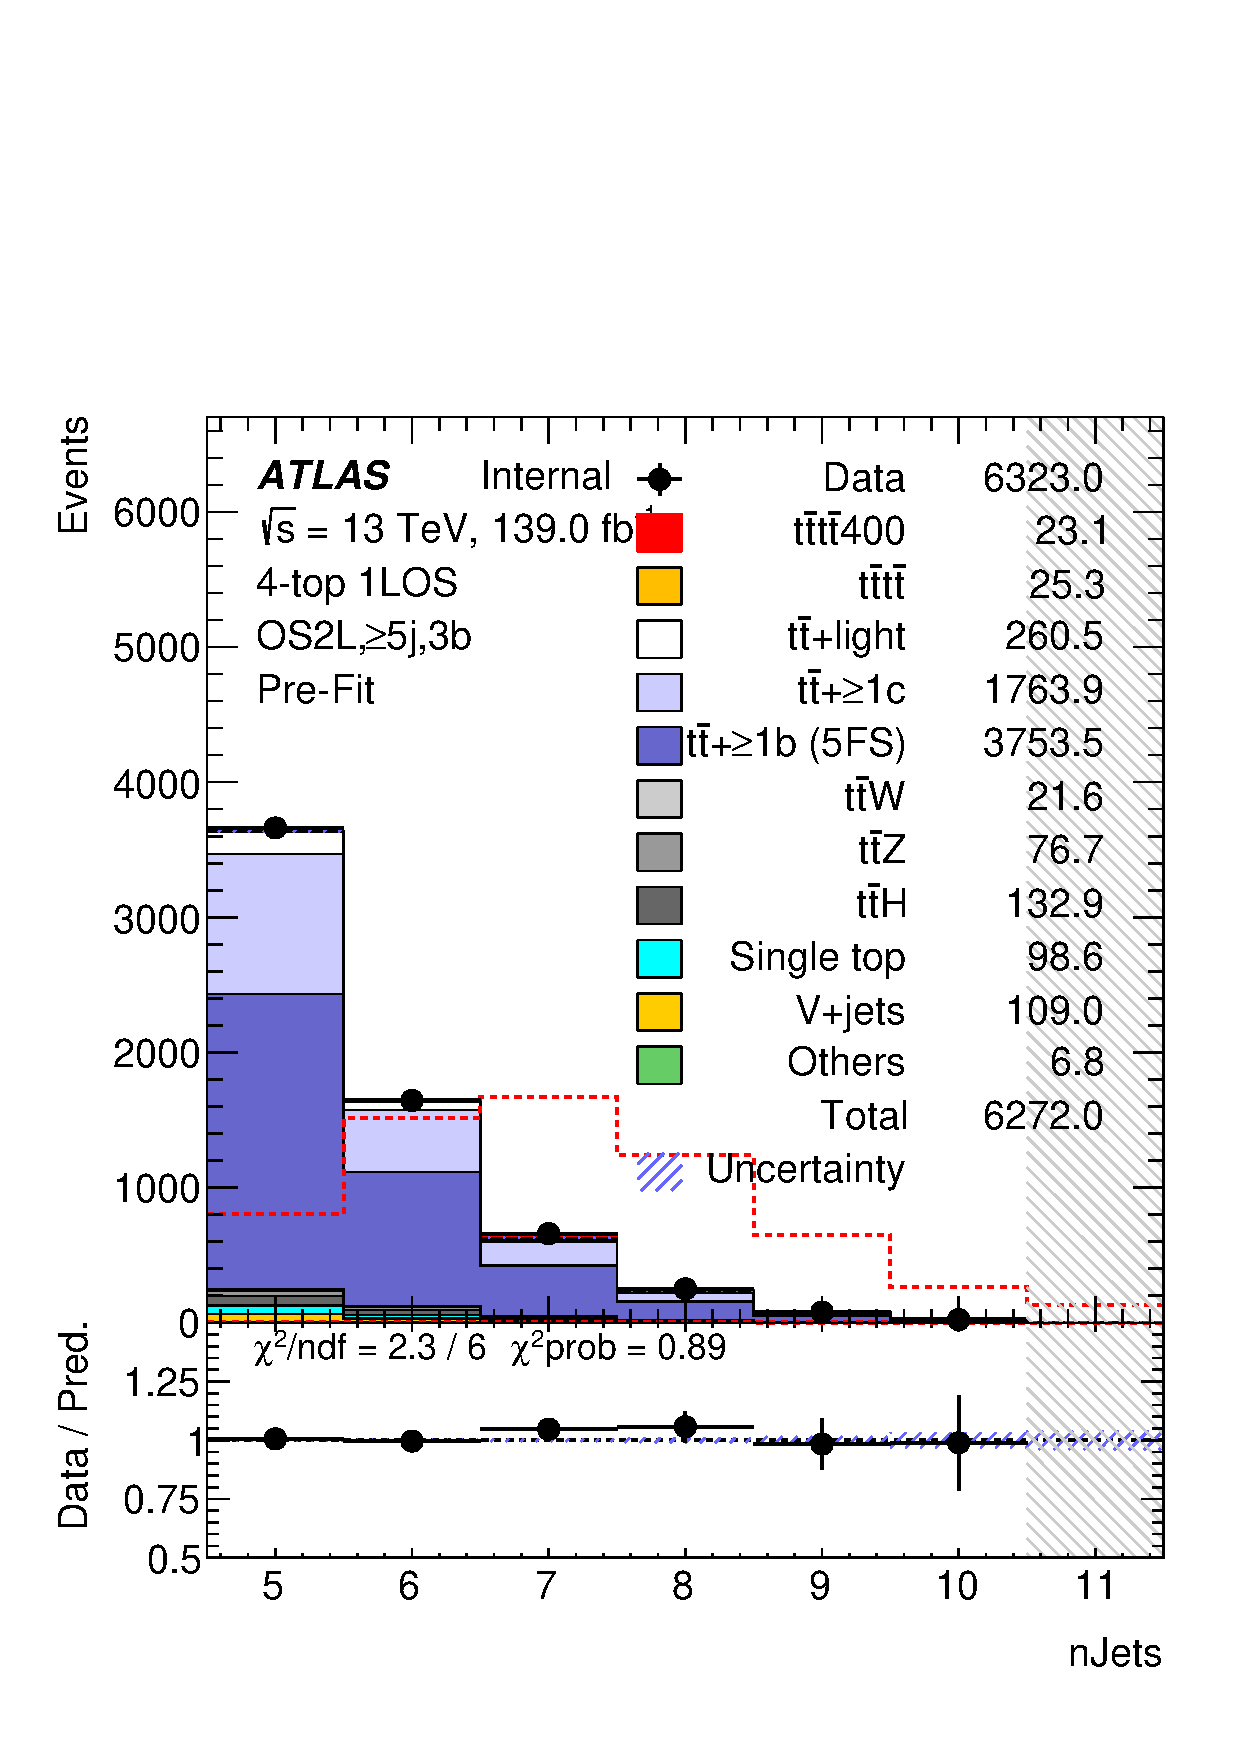
\includegraphics[width=0.25 \textwidth]{figures/fits/4FSvs5FS/GNN/400/Data_to_MC_5FS/val_os2l_ge5j3b.pdf}\\ 
                                                                                                                                                                                 
                                                                                                                                                                                  
      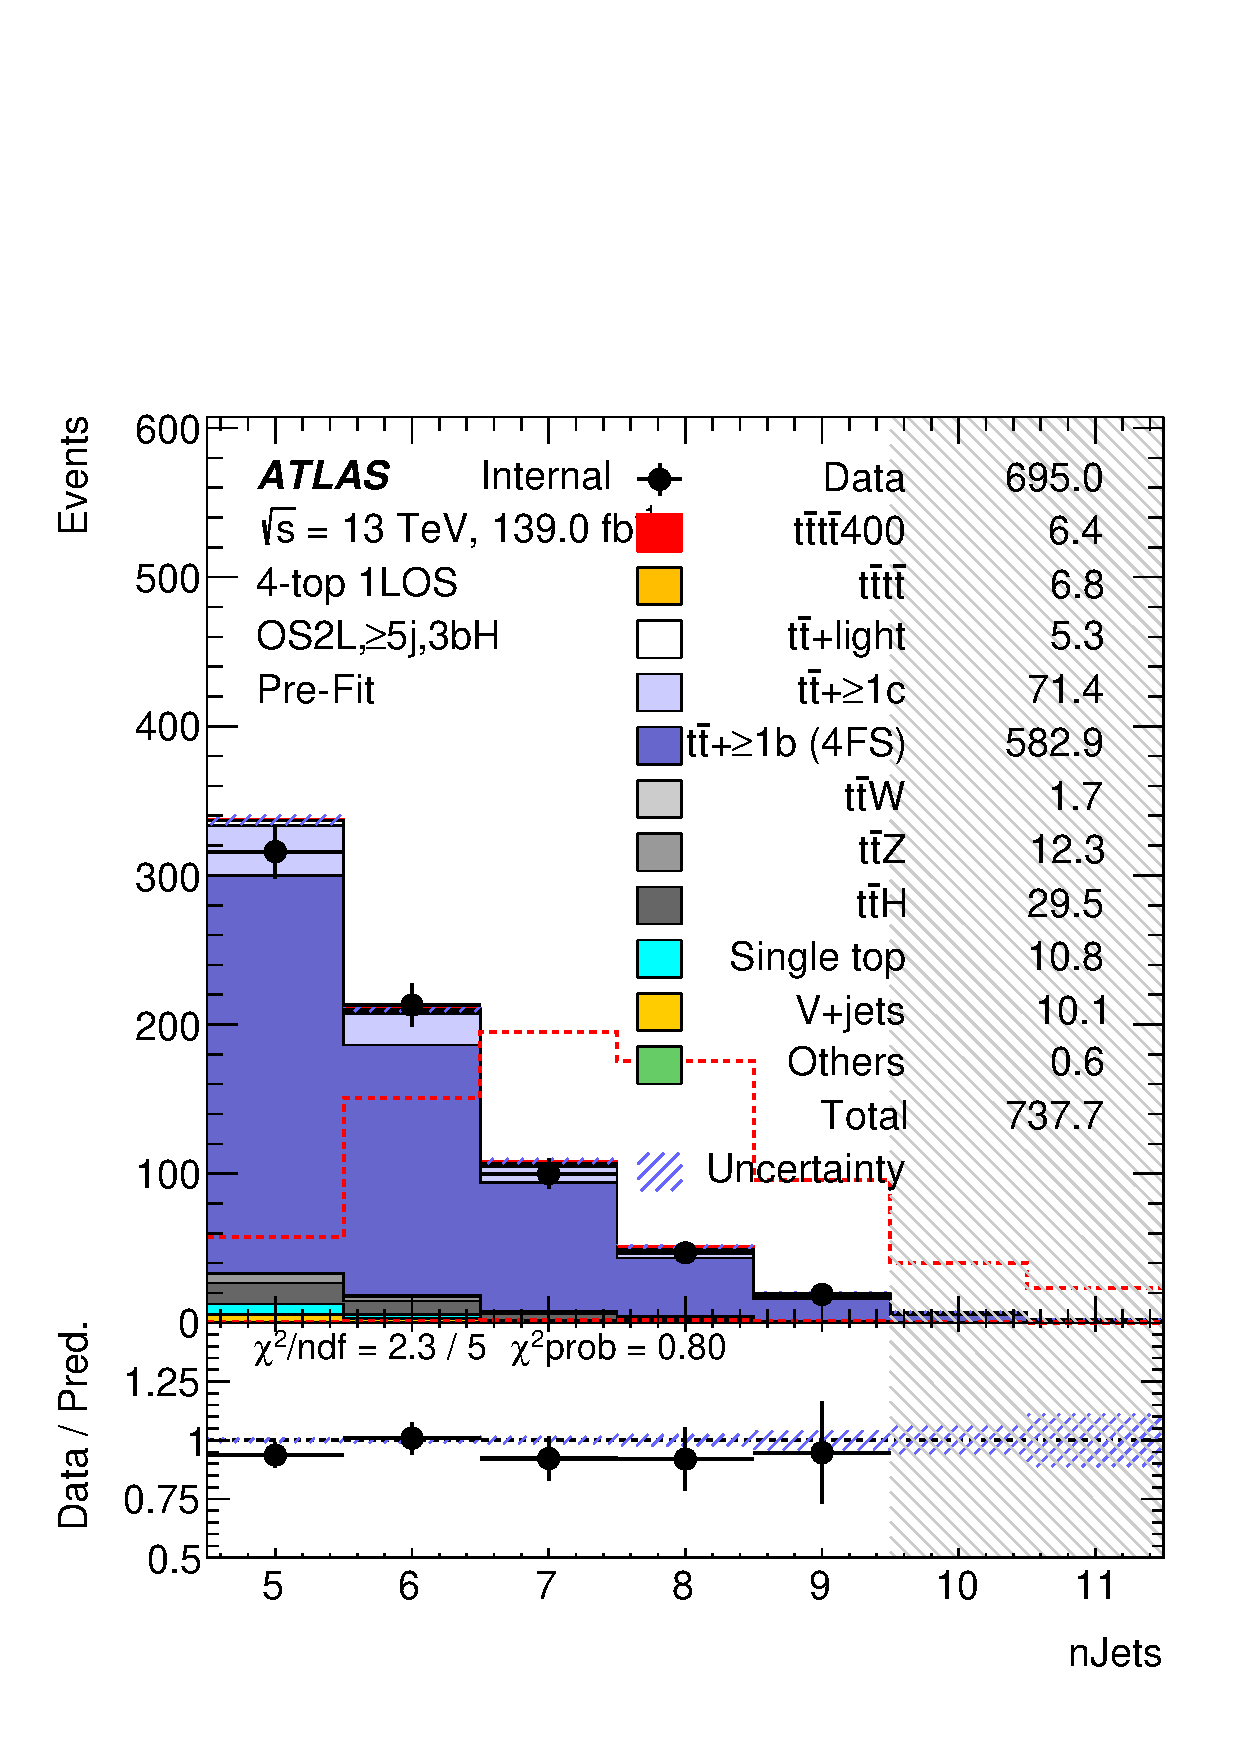
\includegraphics[width=0.25 \textwidth]{figures/fits/4FSvs5FS/GNN/400/Data_to_MC_4FS/val_os2l_ge5j3bH.pdf} &
      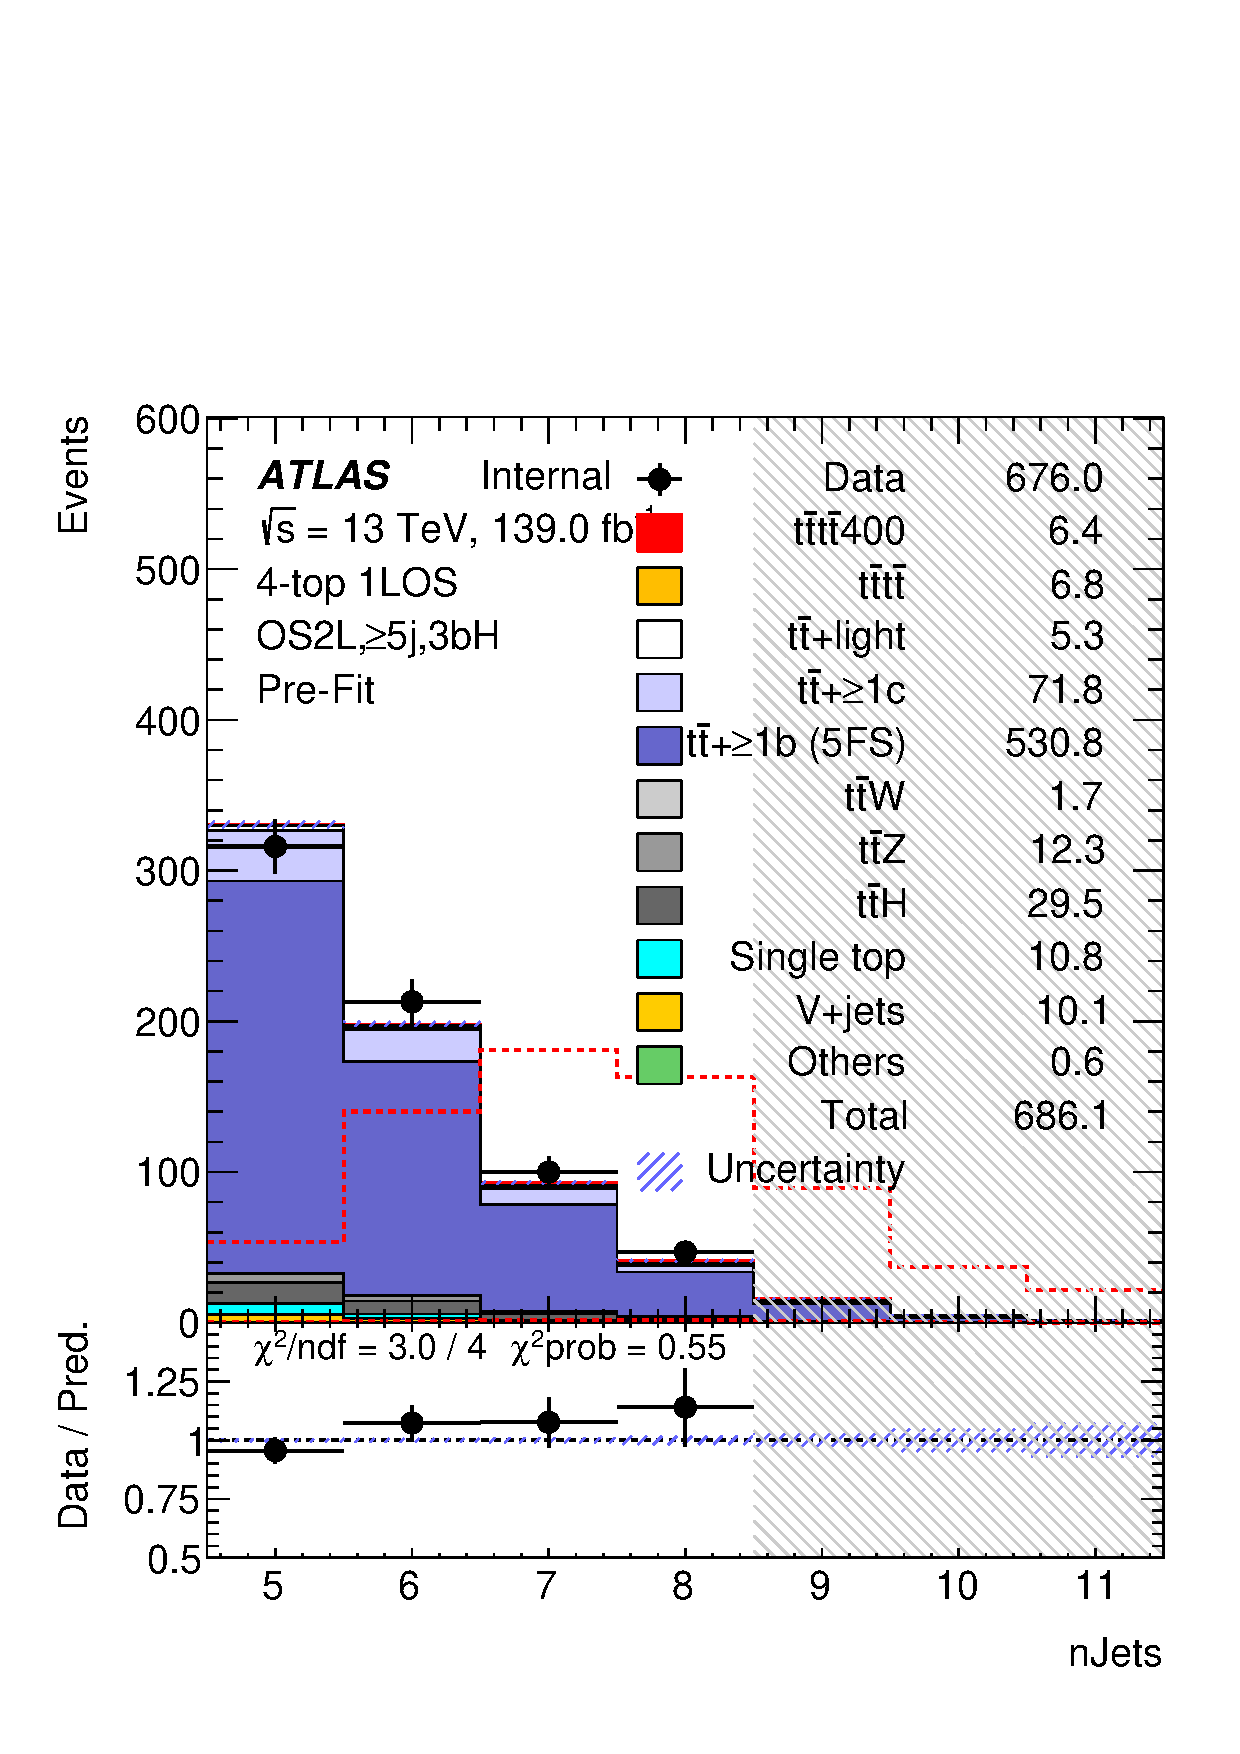
\includegraphics[width=0.25 \textwidth]{figures/fits/4FSvs5FS/GNN/400/Data_to_MC_5FS/val_os2l_ge5j3bH.pdf}& 
      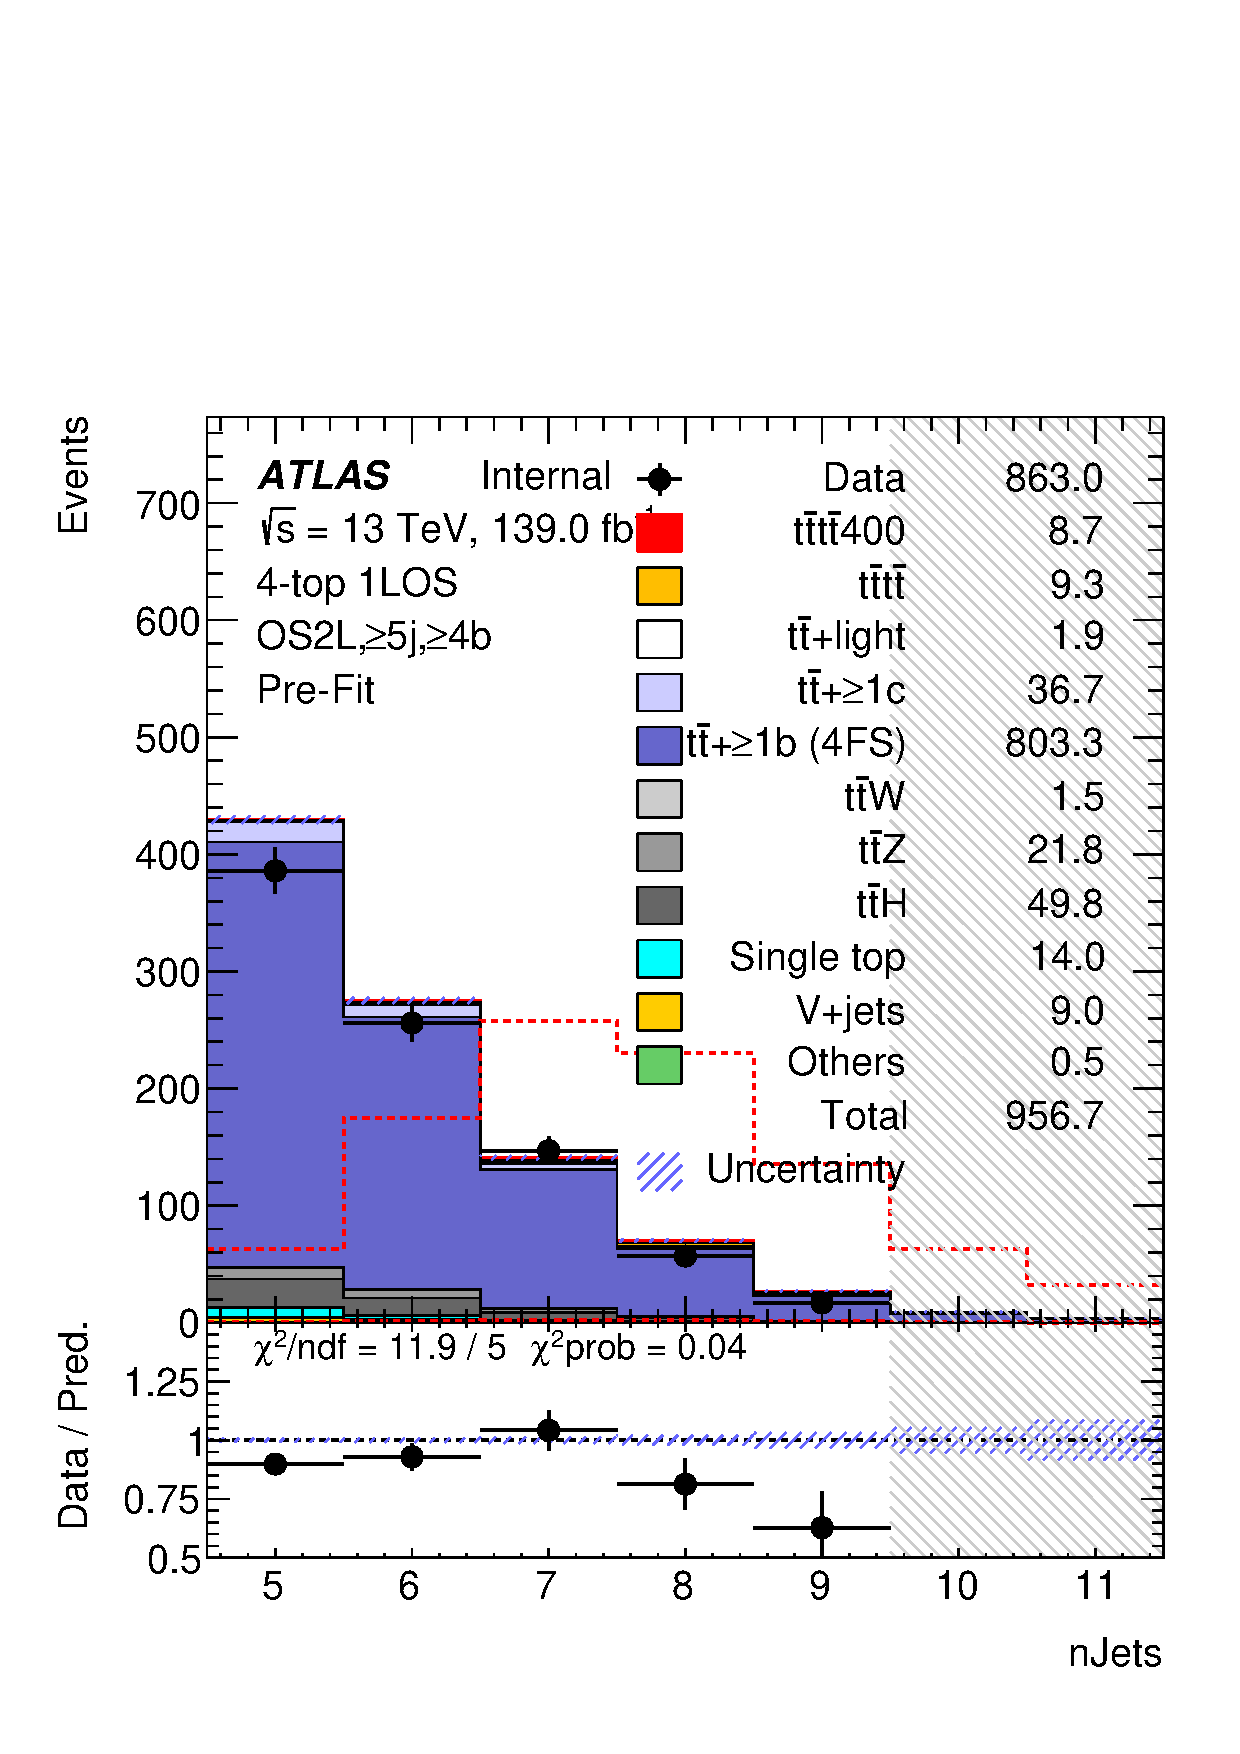
\includegraphics[width=0.25 \textwidth]{figures/fits/4FSvs5FS/GNN/400/Data_to_MC_4FS/val_os2l_ge5jge4b.pdf} &                                                               
      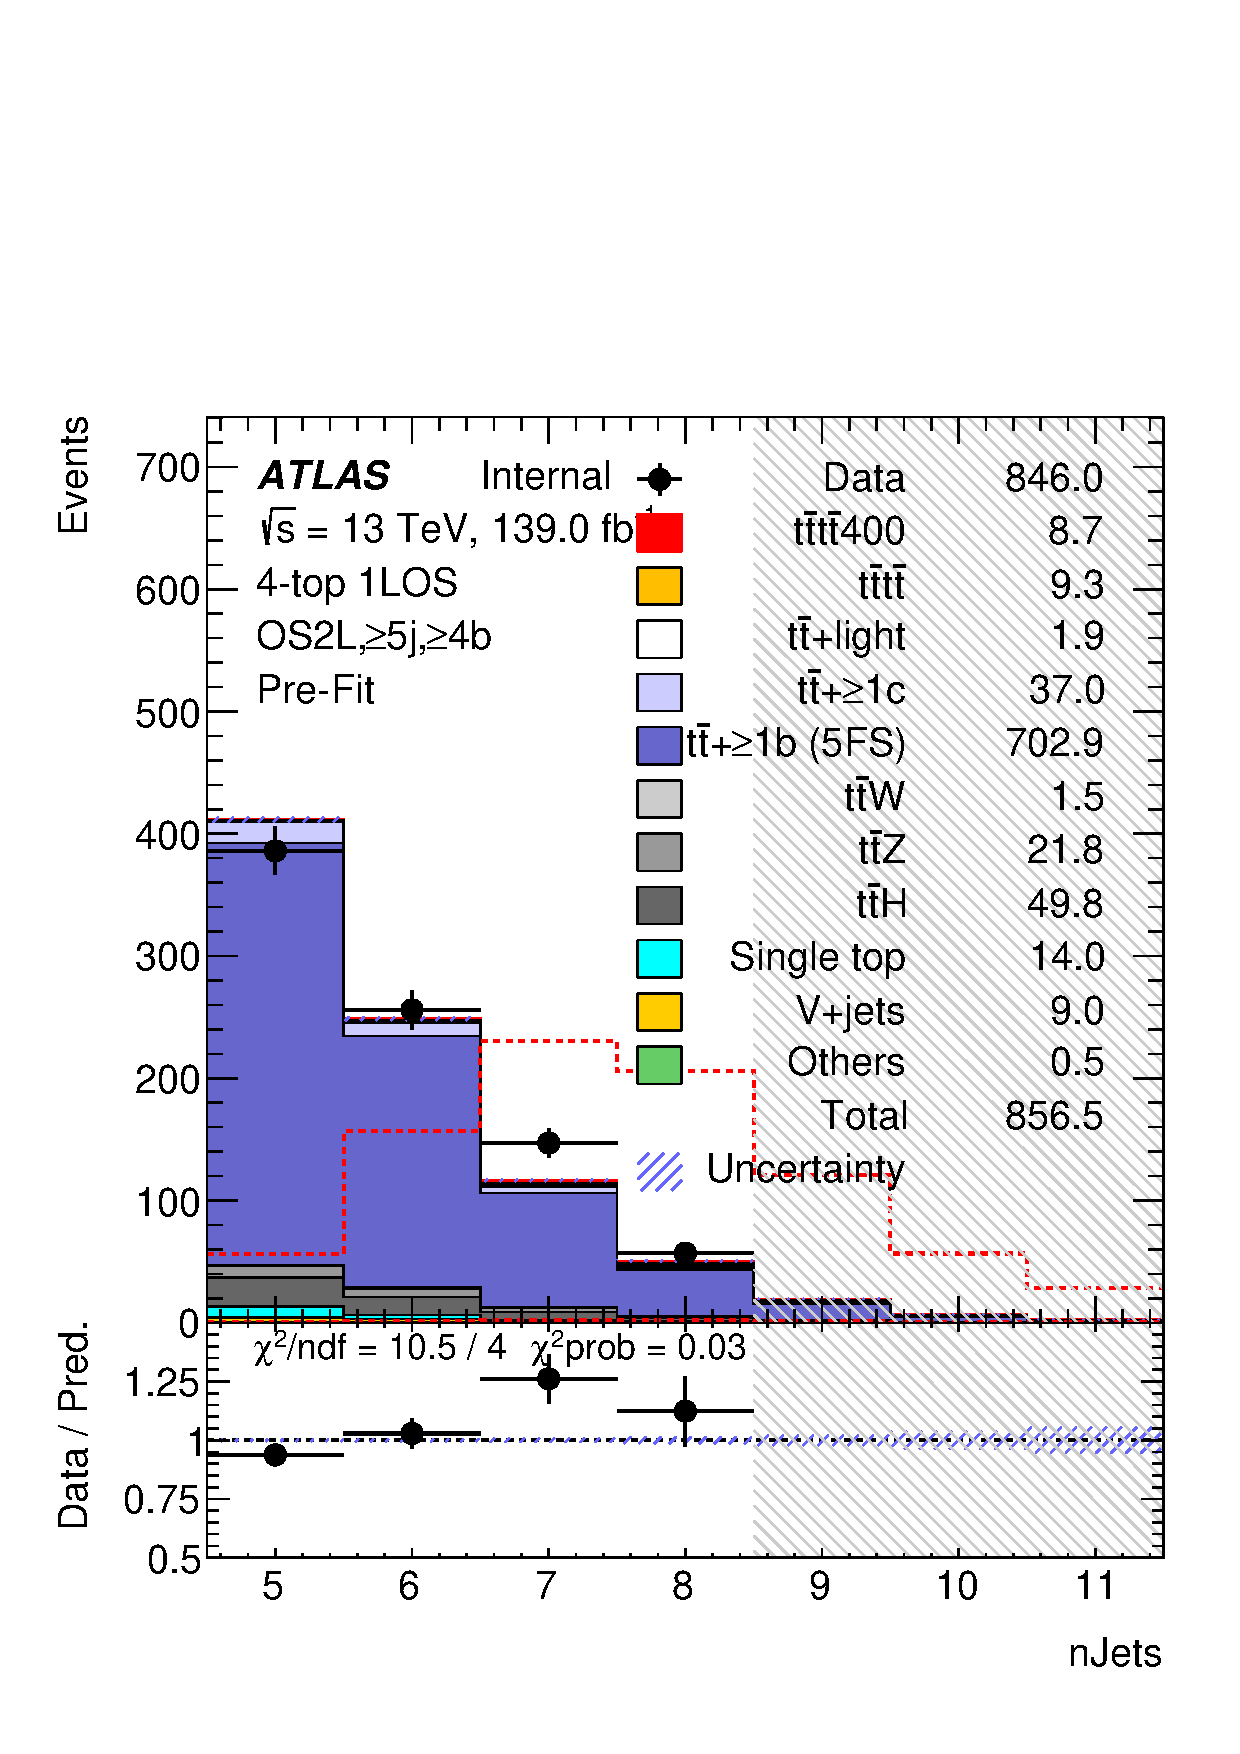
\includegraphics[width=0.25 \textwidth]{figures/fits/4FSvs5FS/GNN/400/Data_to_MC_5FS/val_os2l_ge5jge4b.pdf} \\
                                                                                                                                                                                  
      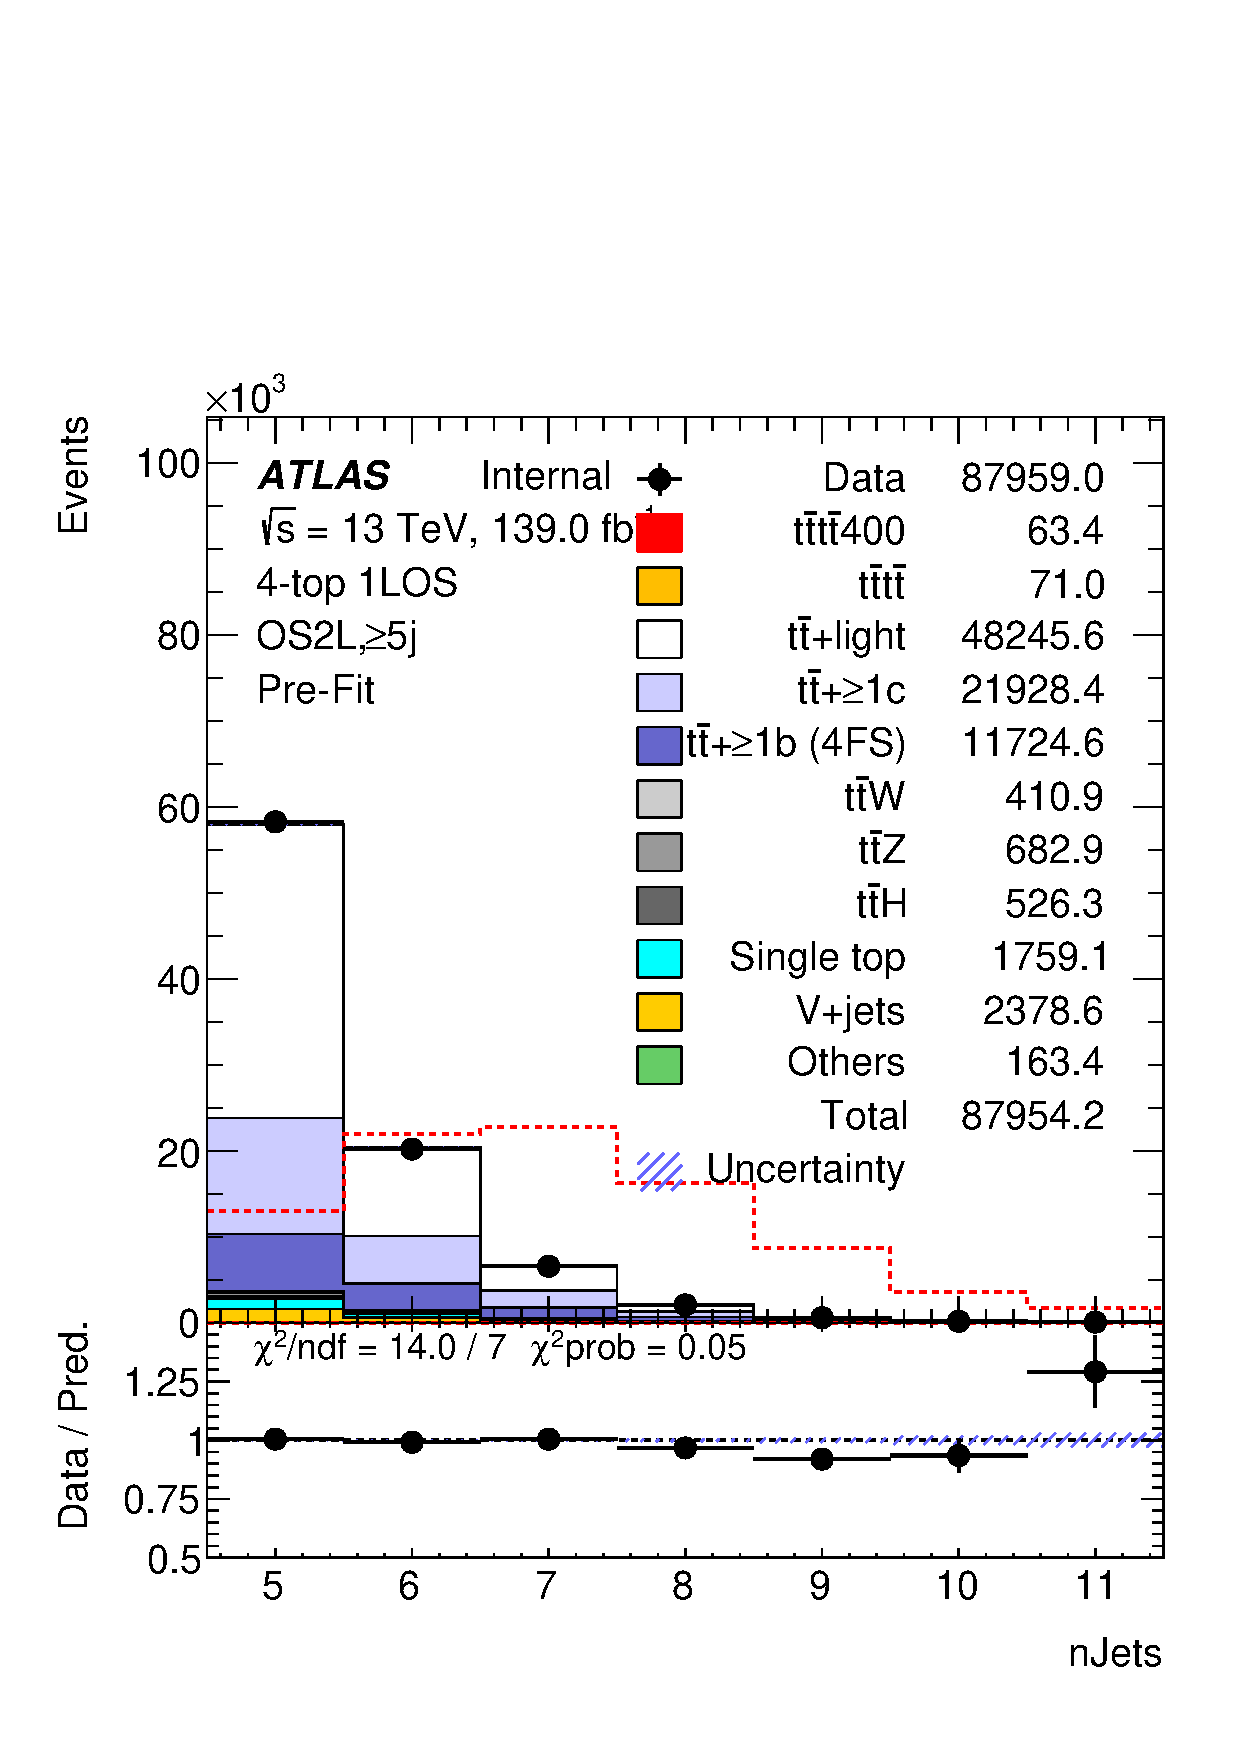
\includegraphics[width=0.25 \textwidth]{figures/fits/4FSvs5FS/GNN/400/Data_to_MC_4FS/val_os2l_ge5j.pdf} &                                                                  
      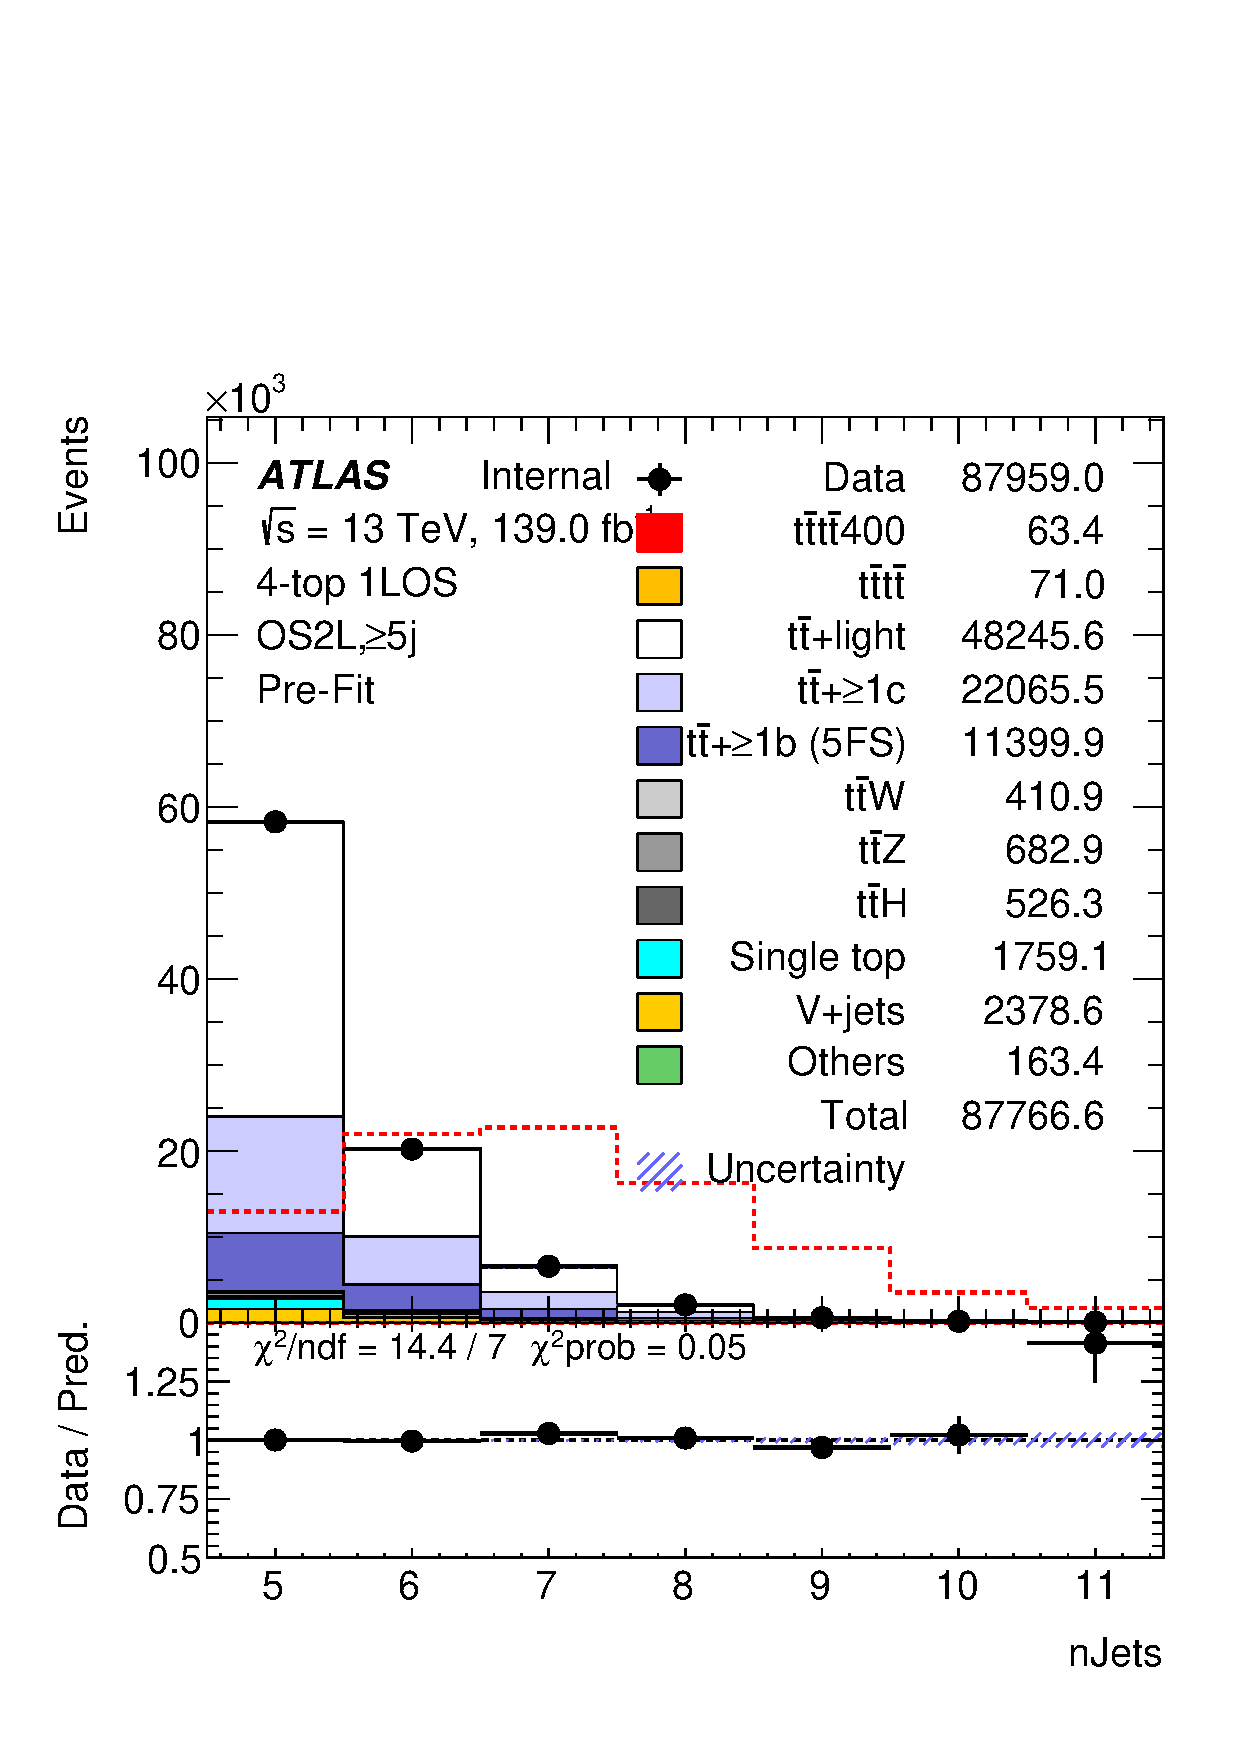
\includegraphics[width=0.25 \textwidth]{figures/fits/4FSvs5FS/GNN/400/Data_to_MC_5FS/val_os2l_ge5j.pdf} \\                                                                 
 
    \end{tabular}                                                                                                                                                                 
                                                                                                                                                                                  
\caption{\label{4FSvs5FS_dataMC_nJets}Pre-fit distributions in 5FS compared with 4FS for 2LOS channel associated with different signal and background samples, compared with data yields in the Njets distribution.}                                                                                                                                                
  
                                                                                                                                                                                 
\end{center}                                                                                                                                                                    
\end{figure}                                                                                                                                                                     
                                                               
